%%%% Copyright 2017 by Sean Luke
%%%% Distributed Under the Apache 2.0 License
\synctex=1

\documentclass{article}
\usepackage{fullpage}
\usepackage{mathpazo}
\usepackage{microtype}
\usepackage{graphicx}
\usepackage{wrapfig}
\usepackage{amsmath}
\usepackage{amssymb}
\usepackage{color}
\usepackage{bm}
\usepackage{gensymb}
\usepackage[hyperfootnotes=false,linktocpage=true,linkbordercolor={0.5 0 0}]{hyperref}

\sloppy

\newcommand\ignore[1]{}

\ignore{
% Alter some LaTeX defaults for better treatment of figures:
    % See p.105 of "TeX Unbound" for suggested values.
    % See pp. 199-200 of Lamport's "LaTeX" book for details.
    %   General parameters, for ALL pages:
    \renewcommand{\topfraction}{0.9}	% max fraction of floats at top
    \renewcommand{\bottomfraction}{0.8}	% max fraction of floats at bottom
    %   Parameters for TEXT pages (not float pages):
    \setcounter{topnumber}{2}
    \setcounter{bottomnumber}{2}
    \setcounter{totalnumber}{4}     % 2 may work better
    \setcounter{dbltopnumber}{2}    % for 2-column pages
    \renewcommand{\dbltopfraction}{0.9}	% fit big float above 2-col. text
    \renewcommand{\textfraction}{0.07}	% allow minimal text w. figs
    %   Parameters for FLOAT pages (not text pages):
    \renewcommand{\floatpagefraction}{0.7}	% require fuller float pages
	% N.B.: floatpagefraction MUST be less than topfraction !!
    \renewcommand{\dblfloatpagefraction}{0.7}	% require fuller float pages

	% remember to use [htp] or [htpb] for placement
}

\newcommand\bump{\vspace{20in}}
\newcommand\name{Flow}
\newcommand\myfrac[2]{#1/#2}
\begin{document}

\noindent {\Huge\bf {\name}}\\[0.5em]
{\large \bf An Open-source, Fully Modular, Multitimbral, Polyphonic Additive Synthesizer\\[0.2em]
Version 5\\[0.2em]
https://github.com/eclab/flow\\\\[0.2em]
By Sean Luke\\[0.2em]
Department of Computer Science\\[0.25em]
George Mason University\\[0.2em]
sean@cs.gmu.edu}

%\setcounter{tocdepth}{1}
\tableofcontents

\clearpage

\section{Introduction}

{\name} is a {\bf fully modular, polyphonic and multitimbral, additive software synthesizer.}  It is free open source and written in Java, and designed to be extended with new, easy to write modules.  You can also create your own patches, then store them as modules to be used in larger patches. 

There have been many additive synthesizers, even semi-modular additive synths, but a fully-modular additive synthesizer is not very common.   It's been fun to write this.  Hopefully this software will inspire others to design similar systems.

{\name} is an academic research experiment and a personal and amateur effort, not a professional product.  Synthesis of the kind attempted here is very costly, and furthermore {\name} tends to emphasize ease of development over efficiency.  This means it'll keep your laptop quite warm and will have lots of odd ends and strings poking out here and there.  {\bf This software is very much in beta.} Absolutely no guarantees are made with regard to its stability or correctness.  It will have a lot of bugs and we will be making regular major, non-backward-compatible changes to it which will break your patches and annoy you.  If you find problems with the software, repeatable bugs, or general irritations, send me mail (sean@cs.gmu.edu).

{\name} was written in Java because it is highly portable and still pretty fast: perhaps using this synthesizer will convince you of this.  You can run a great many modules at once in a patch as necessary.  But because {\name} is in Java, it must be a standalone application, not a VST or AU.  The software should run fine on Windows, OS X, and Linux, though it was developed for OS X and has not been tuned or tested much on the other platforms to date (especially not Windows).


\subsection{A Bit on Additive Synthesis}  
\label{additivesynthesis}

\begin{wrapfigure}{r}{3in}
\vspace{-1em}
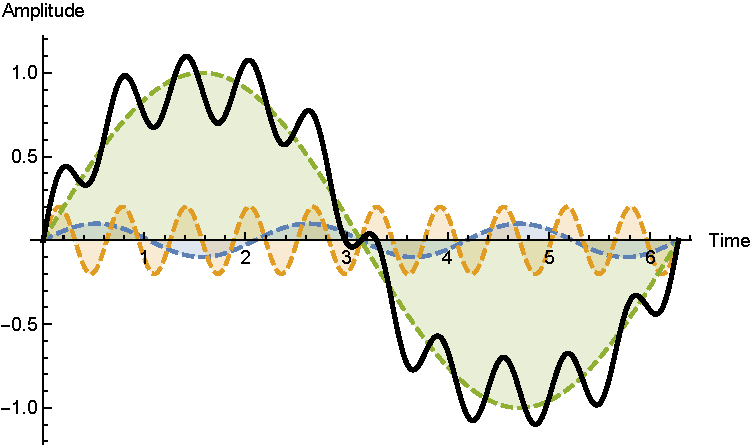
\includegraphics[width=3in]{sinewaves}
\caption{Three sine waves (colored) and the result of adding them up (in bold).}
\label{sinewaves}
\vspace{-1em}
\end{wrapfigure}

An additive synthesizer is a synthesizer which produces sounds by {\it adding up} multiple sine waves of different frequencies, amplitudes, and phases.  Each such sine wave is called a {\bf partial}, because it is in some sense a {\it part} of the final wave.

Consider Figure~\ref{sinewaves}, which shows three sine waves in green, orange, and blue.  These sine waves are differing in their {\it frequency} (how fast they go up and down), and in their {\it amplitude} (how far they go up and down).  If you add the three sine waves up, you get the wave shown in bold.  In fact, it's easily shown that in theory you can synthesize {\it any wave} by adding up the right combination of sine waves.

Notice we didn't mention {\it phase}.  Phase is the horizontal shift in the sine wave, as shown in Figure \ref{phases}.  As it turns out, humans often can't easily distinguish between sounds whose partials only differ in phase relative to one another: we just don't have the hardware built-in to do it.\footnote{While this is certainly true for high- and mid-pitch sounds, it isn't entirely true for bass sounds: a low-frequency square wave (for example) sounds pretty different\,---\,buzzier\,---\,than one whose partials have randomly-assigned phases.}   As a result,  many additive synthesizers, including {\name}, don't consider phase in order to simplify matters.

If we only consider frequency and amplitude, we can chart our three sine waves as shown in Figure~\ref{partials}: showing the amplitude of each partial by frequency.  Notice that the \(Y\) axis is still Amplitude, but the \(X\) axis has changed from {\it time} to {\it frequency}. For this reason, thinking of a sound in this fashion is known as casting the sound into the {\bf frequency domain}; whereas thinking of a sound as a wave in the traditional way (Figure~\ref{sinewaves}) is known as considering it in the {\bf time domain}.  While we have been trained to think of sound waves in the time domain: in fact our brains receive sound information in the frequency domain: hardware in our ears first breaks out the sounds into high and low frequencies before our brains even get them.

\begin{wrapfigure}{r}{3in}
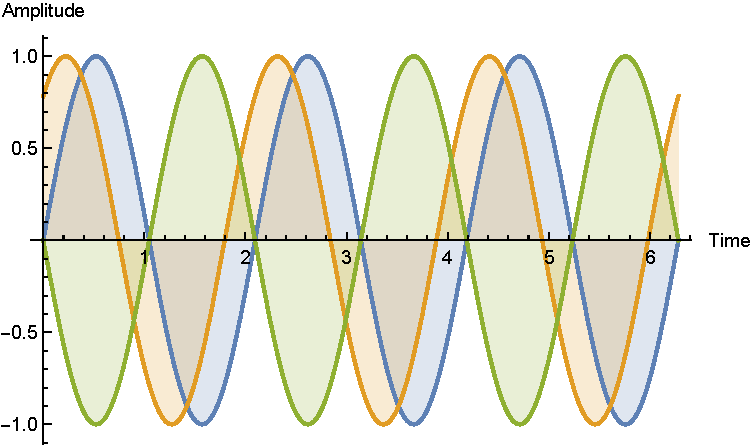
\includegraphics[width=3in]{phases}
\caption{Three sine waves which differ only in phase.  Note that the green and blue waves differ by so much that they have become inverses.}
\label{phases}
\vspace{-1em}
\end{wrapfigure}

Figure~\ref{partials} is more or less the same basic kind of data that sound modules in {\name} send to one another: a list of partials, where each partial has a frequency and an amplitude.  At the end of the day, the final list of partials is sent to the output facility to have their sine waves added up and emitted as a sound wave.

The lowest partial is commonly known as the {\bf fundamental},\footnote{This is kind of a lie.  Technically the fundamental is the lowest or ``first'' partial: but the term {\it fundamental} is also often used to describe the {\it loudest} partial, or the one whose frequency we think of as the pitch of the sound.  These three things usually coincide, but for some musical instruments they're not the same.  For example, in organs the fundamental is the tone we associate with the pitch: but there may exist one or two partials {\it lower} than it.  This is also the case for bells, where the fundamental (also called the {\it strike tone}) is usually higher than at least one partial known as the {\it hum tone}.  In a bell, there are often partials louder than the fundamental as well, and in fact the fundamental might not even exist\,---\,we think we're hearing a note, but in fact there's no partial there!  Bells are weird.   For simplicity, when {\name} refers to the fundamental, it means the lowest partial.}  and the other partials are often known as {\bf overtones}.  It so happens that a large number of physical things which we perceive as ``musical sounding'' (such as strings or flutes) produce partials which, by and large, have a certain interesting feature: they are all integer multiples of the fundamental.  That is, if the fundamental is at frequency \(f\) the next partial will be at frequency \(2f\), the next partial will have frequency \(3f\), and so on (and conveniently in Figure~\ref{partials} this was the case).  Partials which fall along these integers are known as {\bf harmonics}.  

\begin{wrapfigure}{r}{3in}
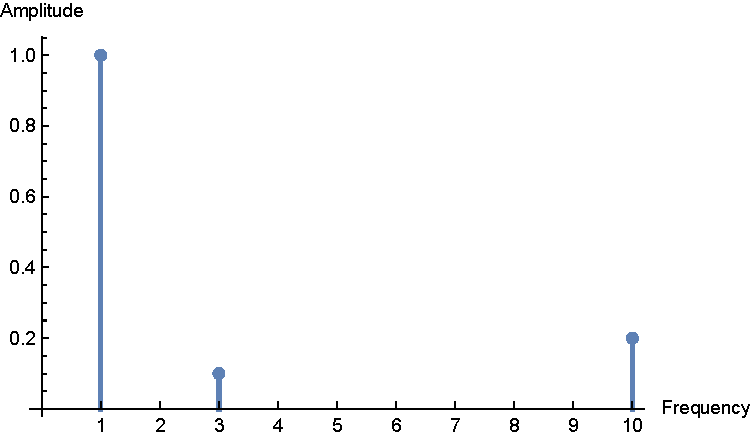
\includegraphics[width=3in]{partials}
\caption{Three sine waves (colored) and the result of adding them up (in bold).  Compare to Figure \ref{sinewaves}.}
\label{partials}
\end{wrapfigure}

Many early (and current!)\ additive synthesizers, such as the Kawai K5 and K5000, simply assumed that all sounds of interest would be generated using harmonics, not arbitrary partials.   {\name} does not make this assumption: you can have partials at any frequency you like.  But you will see harmonics in many places, as they are common and useful.

In {\name}, if you adjust partials so that they are all harmonics, with no gaps among the integers, this procedure is called {\bf standardizing} them.  Another term you'll see: if you adjust the partials so that their amplitudes add to 1.0, this is called {\bf normalizing} them.  Some modules can do standardization or normalization as an option.

(Useful) partials can have any frequency from 0 up to the {\bf Nyquist limit} of a digital sound wave.  The Nyquist limit is the highest frequency a digital representation is capable of producing: it is half the sampling rate.  So if the audio rate is 44100 Hz (as is the case for {\name}, and of course, for CDs), then the highest possible frequency is 22,050.

\subsection{Fully Modular Additive Synthesis}  Additive synthesis is viewed as a sort of holy grail of synthesis: because you can generate all sounds in an additive fashion in theory, additive synthesis is in some sense an ``optimal'' way to doing synthesis: but it has a problem which prevents it from being easily used in reality.   And that problem is: the classical approach to additive synthesis involves a very, very large number of tedious parameters.  Sound waves have many hundreds or thousands of partials, each with a frequency and amplitude and maybe phase: and as sounds change and evolve over time, so do all those values.  And so a synthesizer in which you set all the partials independently will have a great many parameters to set.  Consider: the Kawai K5000 had 126 harmonics, each with a base amplitude and {\it its own envelope} which specified how it changed over time.  This meant that the Kawai K5000's patches had on the order of a thousand parameters.\footnote{I'm not denigrating the K5000!  The K5000 was one of the most incredible and awe-inspiring synthesizers in history.}

An alternative approach, taken by software tools such as Harmor/Harmless, Razor, and Loom,\footnote{Harmor and Harmless are trademarks of Image-Line Software.  See https:/\!/www.image-line.com/plugins/Synths/Harmor/  and https:/\!/www.image-line.com/plugins/Synths/Harmless/\qquad Razor is a trademark of Native Instruments, Inc.  You can find Razor at https:/\!/www.native-instruments.com/en/products/komplete/synths/razor/\qquad And Loom is a trademark of inMusic Brands.  You can find Loom at http:/\!/www.airmusictech.com/product/loom-ii}
is to create a series of modules which either generate sets of partials or modify existing partials, and then to arrange them in an assembly line, routing partials from one module to the next, until a sound is emitted at the end.  The idea is that instead of directly manipulating partials and envelopes, you're using operations (the modules) designed to sculpt away at the partials.  But because you can't wire up the modules in any fashion, these tools generally use a kind of {\bf semi-modular synthesis} approach.  

{\name} is in contrast closer to a {\bf fully modular synthesis} approach: you can organize as many modules as you like, and wire them up however you like, just like a hardware modular synthesizer. Since they're not in a line, modules can be fed from, and feed into, {\it multiple} other modules.  There's no reason you can't have modules wired up in cycles or other patterns.  And just like in a hardware modular synthesizer, if you don't wire the modules up at all, you don't get any sound. 

Note however that unlike a classical fully-modular synthesizer, a software synthesizer like {\name} can easily be (and is) {\bf polyphonic} and {\bf multitmbral}, and you can save and load patches.  And of course, unlike a traditional modular synthesizer, {\name} is {\bf additive}.

{\name} has another powerful trick up its sleeve: after you have saved your collection of wired modules out as a {\bf patch}, you then have the option of loading that patch to operate as a {\bf self-contained module in another patch!}  When a patch is loaded in this way, it is called a {\bf macro}.  And yes, you can have macros which contain macros which contain macros.


\subsection{Specifications}

At present {\name} has the following specifications.  They may change:

\begin{center}
\begin{tabular}{rl}
Number of Partials&64, 128, or 256, user-selectable.  Phase is disregarded.\\
Polyphony&1--32, user-selectable.\\
Multitimbrality&Up to (at present) 32 unique sounds.\\
Sampling Rate&44,100 Hz\\
Audio Bit Depth&16 bit\\
Channels&Mono (that is, not stereo)\\
MIDI Features&MPE, Clock, Channel and Polyphonic Aftertouch, Pitch Bend, NRPN, RPN, CC\\
\end{tabular}
\end{center}


\bump

\begin{figure}[t]
\begin{center}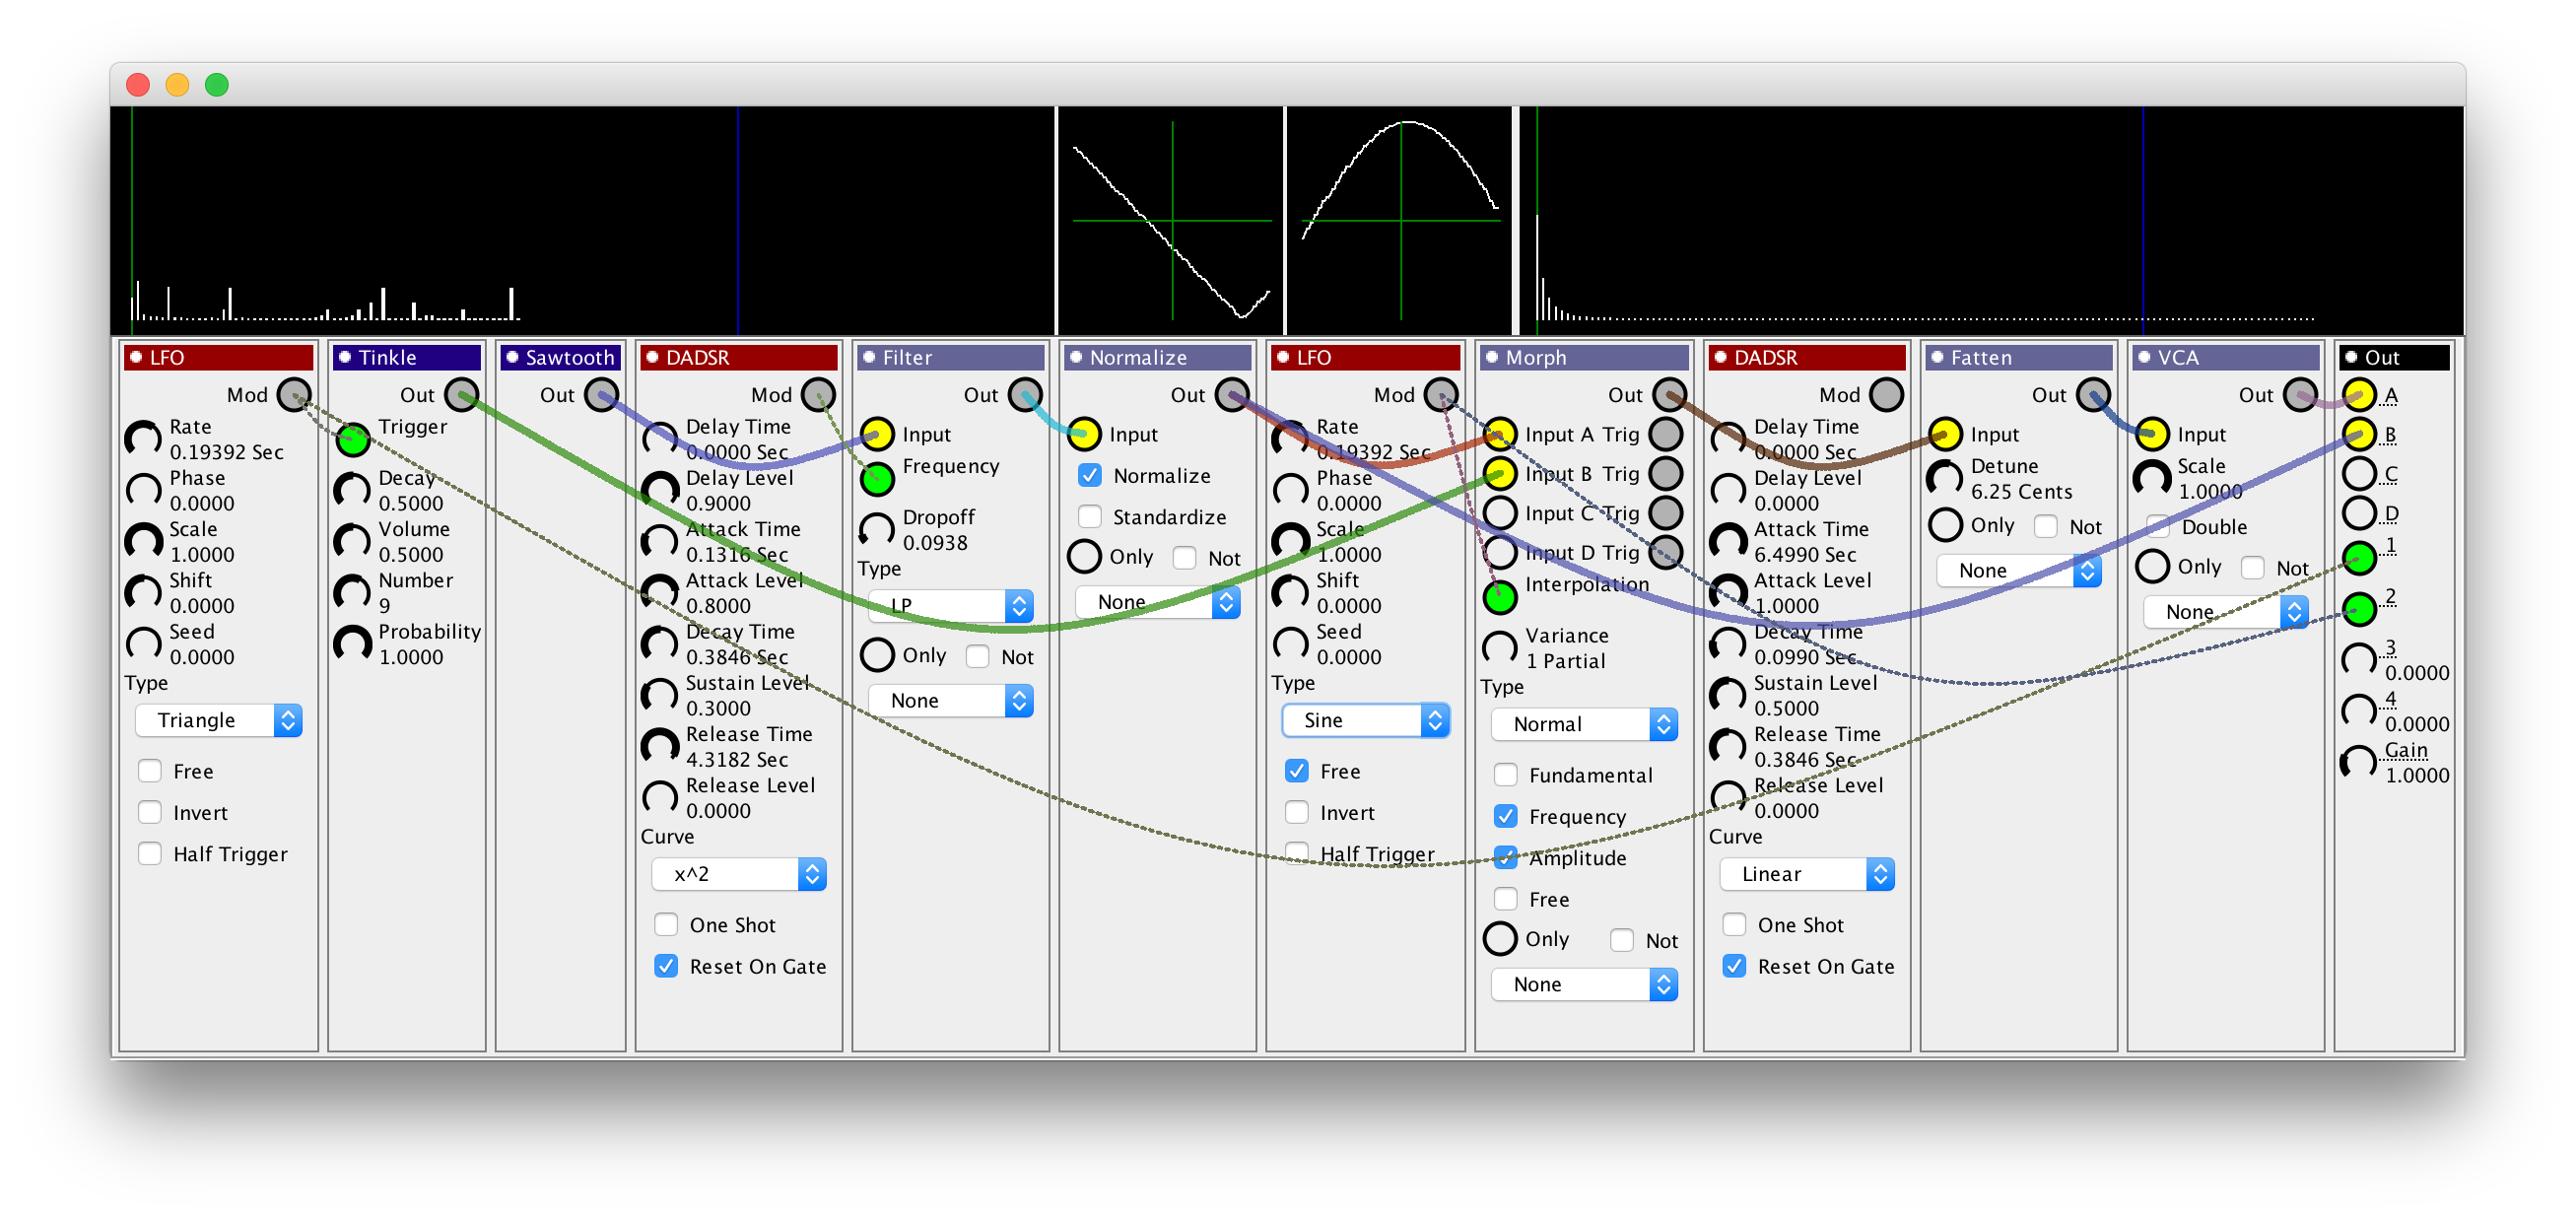
\includegraphics[width=6.5in]{screenshot}\end{center}
\vspace{-3em}
\caption{An Example Patch}
\label{screenshot}
\end{figure}


\section{Using {\name}}

After you fire up {\name}, you're presented with a near-empty {\bf rack} (except for the {\bf Out} module) and can start adding {\bf modules} to it.  Then you tweak the parameters of modules and wire them up by dragging from output jacks to input jacks or to dials.  The result might look something like the example patch in Figure~\ref{screenshot}.

If you look carefully at Figure~\ref{screenshot}, you'll see that there are not only twelve modules, but also two wide black rectangular regions called {\bf displays}, and two small squarish black regions called {\bf oscilloscopes}.  Displays show partials in the same manner as Figure~\ref{partials}, and oscilloscopes display modulation signals.

\subsection{Tuning Parameters}
First things first.  {\name} is very computationally expensive and benefits from tuning for your computer speed.  If your computer can't keep up with Flow's demands, you'll hear a {\bf glitch}.  This is a pop or a buzz in the audio stream, and will be accompanied by the {\bf Out} module (the top-right module shown in Figure \ref{screenshot}) coloring its black title bar red and saying ``Glitch''.  A glitch occurs when Flow can't keep the audio buffer filled fast enough, so your computer is forced to start filling it with zeros.  You don't want that.

How do we tamp down glitches?  By playing with a few parameters. If you select {\bf Tuning Parameters} from the {\bf Options} menu, you can at present change three parameters.  Pressing {\it Okay} or {\it Reset} (which resets to defaults) will change the parameters for the {\it next} time you run {\name}, not the current session. 

\begin{itemize}
\item {\bf Polyphony} (1--16, default: 8)\qquad This is the number of voices the synthesizer can play at once.  More voices incurs a higher load.
\item {\bf Audio Buffer Size} (default: 1152, which is crummy, but the best Java on the Mac can do)\qquad This is the size of the audio buffer that {\name} keeps filled for your operating system to tap into to generate sounds.  You want a low buffer if you can (much less latency); but a bigger buffer makes it easier for Flow to keep up.  Some operating systems require a large buffer size: for example, OS X typically needs at least 1152 . On Linux you can get away with much smaller buffers: see the Linux portion of Section~\ref{connecting} for more information.  I can't help you much regarding Windows.

\item {\bf Partials} (64--256, default: 128)\qquad This is the number of partials passed around from module to module.  More partials will produce a richer sound, particularly in bass notes, but incur a much higher load.

\item {\bf Voices Per Thread} (1, 2, 4, 8, 16, default: 8)\qquad This is the number of voices which will be assigned to a single CPU thread in the partials-updating stage of synthesis.  More voices per thread means fewer threads.  You'd like as many voices assigned to a given thread as possible, because switching threads incurs significant computational overhead.  However if you have too many voices on a thread, then they cannot take advantage of the parallelism afforded by your laptop's nifty multi-core CPU and you won't have fast partials updates.  Also if you have very few voices per thread, then you'll have many more threads in the partials-updating stage and this may nudge out the critical output threads, resulting in more glitches.  You have to find a balance.  

\item {\bf Outputs Per Thread} (1, 2, 4, 8, 16, default: 2)\qquad This is the number of voices which will be assigned to a single CPU thread in the sound-output stage of synthesis.  More voices per thread means fewer threads.  You'd like as many voices assigned to a given thread as possible, because switching threads incurs significant computational overhead.  However if you have too many voices on a thread, then they cannot take advantage of the parallelism afforded by your laptop's nifty multi-core CPU and you will glitch because Flow can't service the audio output fast enough.  You have to find a balance.  
\end{itemize}

\subsection{Adding, Moving, Copying, and Closing Modules}  Modules are added to the rack by choosing them from the {\bf Modules} menu.  You can move a module to another location by dragging its title bar.  You can also copy a module to another location by dragging its title bar while holding the Control key (on the Mac, you can also hold the Option key).  Finally, you can delete a module by clicking on its close box: the little white dot to the left of its title.

By default, modules are added to the beginning of the rack.  You might find this annoying.  If you would prefer modules to be added to the end of the rack (just before the Out module), choose {\bf Add Modules At End} from the {\bf Options} menu.

\subsection{Partial and Modulation Signals}  Modules can send and receive two kinds of signals.  First, a module can send or receive {\bf sets of partials} to/from other modules.  Since this is an additive synthesizer, a set of partials is essentially a sound being emitted from a module.  Additionally, a module can send or receive a {\bf modulation signal}.  This is a single number, ranging from 0 to 1, which can change over time.  Modulation signals are used to change parameters in modules in real time.  

\begin{wrapfigure}{r}{2.6in}
\vspace{-1em}
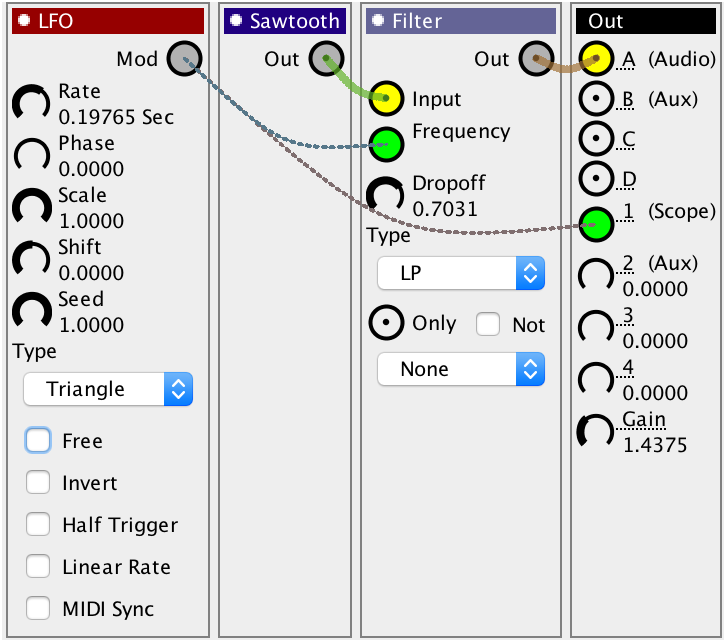
\includegraphics[width=2.6in]{simplepatch.png}
\caption{A Simple, and Terrible, Patch}
\vspace{-1em}
\label{simplepatch}
\end{wrapfigure}

Modules can send any number of partials and modulation signals, and they can receive any number of the same.  But some modules are intended {\it primarily} to {\bf create modulation signals} (their title bars are red), to {\bf shape incoming modulation signals and emit new versions} (light red title bars), to {\bf create partials} (blue), or to {\bf shape incoming modulation signals and emit new versions} (light blue).  A few system-level modules, such as the {\bf Out} module, have black title bars.  Macros (see Section~\ref{aboutmacros}) have green title bars.

Figure~\ref{simplepatch} shows a very simple patch: a Sawtooth wave run through a low pass filter whose cutoff frequency is modulated by a sine-wave LFO.   Notice the special module {\bf Out}.  If you attach a module to the jack labelled {\it A (Audio)} on this module, then the module's partials will be used to produce the final output sound.  We've attached the jack {\it Out} on the module {\bf Filter} to the jack {\it A (Audio)} in the module {\bf Out}, so the Filter's output is being routed directly to audio.   For more information on the capabilities of the {\bf Out} module, see Section~\ref{outmodule}.

The Filter is also receiving partials (which it's filtering).  These partials are coming from the {\bf Sawtooth} module.  Its {\it Out} jack is attached to the {\bf Filter}'s {\it Input} jack.  Notice that the wires connecting Partials input and output jacks are thick, solid (random) colors.  You make these wires by just dragging from an output jack to your chosen input jack.

In contrast, modulation wires are thin and dashed.  Note the {\bf LFO} has two such wires coming out of its {\it Mod} jack and leading to the {\bf Filter}'s {\it Frequency} jack.  We have set up the LFO to {\bf modulate} the cutoff frequency of the filter.
The jack is also connected to a jack in {\bf Out} called {\it 1 (Scope)}: this will cause the modulation to appear on the primary oscilloscope.  

While the input jack for partials is a circle, what is the input jack for modulations?  The answer is: it's a dial.  If you haven't connected it, it appears as a dial and you can simply set its value.  If you connect it, it turns into a connected circle and receives its values as modulation. 

You disconnect a wire by clicking on the input jack it's connected to.  And you change the color of a wire by clicking on its output jack.

\paragraph{Patching Backwards}  Typically you'd wire a module to send information on to another module further to its right in the Rack.  But there's no reason you can't wire a module to send to another module to its {\it left}, and there are often good reasons to do so.  However you should be aware of one minor consequence of this.  Every time the Rack wants to get the latest partials to send the audio output, it does by pulsing modules left-to-right.  A module can extract information from other modules only when it's being pulsed.  Normally this is fine: if module \(X\) gets information from module \(Y\) to its left, by the time \(X\) is extracting information from \(Y\), \(Y\) has already been pulsed and so is ready to provide the latest information.  But if module \(X\) is getting information from module \(Z\) to its {\it right}, \(Z\) has not been pulsed yet and so its information will be old.  How old?  By default, it'll be typically about 32 samples, or about 0.725~ms old.  If you chain a bunch of modules backwards like this in a line, this delay starts multiplying.   With about 5 modules wired backwards in a chain like this, you'd be over 3~ms, which is getting into the realm of human detection.\footnote{Perhaps it's the effect you were aiming for!} 

\subsection{Setting Values in Dials}

If an input jack for a modulation isn't connected, it appears as a dial: you can fix its value to anything between 0.0 and 1.0 inclusive by dragging the dial up or down.  Some dials won't show values between 0.0 and 1.0, but rather give a more informative value display like ``3.23 sec''  or ``2023 Hz''.  But underneath they're always just values from 0 to 1.

There are some other options available on setting these dials.  

\begin{itemize}
\item If you double-click on the dial, a menu will pop up with common settings for you to choose from.  Importantly, if you double-click on rate or time dials in LFOs or various Envelopes, these settings will correspond to note speeds if you were playing at 120 BPM (or whatever rate the MIDI Clock is running~at).
\item If you hold the {\bf Alt} or {\bf Option} key down and then drag, your resolution will be 4x.
\item If you hold the {\bf Control} key down and then drag, your resolution will be 16x.
\item If you hold the {\bf Control} {\it and} the {\bf Alt} or {\bf Option} keys down and then drag, your resolution will be 64x.
\item If you double-click on the dial while holding down the {\bf Shift} key, or if you double-click on the dial using the right mouse button, a dialog box will pop up which allows you to enter a precise value.
\end{itemize}

\subsection{Triggers}

Modulation signals not only carry a time-varying number, but also can send a {\bf trigger event}.  Various modules use incoming modulation triggers to pulse them.  When a trigger occurs depends on the modulating module: for example an LFO sends a trigger every time it completes a single wave. 

In a classic modular synthesizer, control signals take the form of either gates or control voltage (CV), hence the term ``gate/CV''.  In a very real sense, modulation and triggers together perform the same function as gate/CV, albeit combined into a single wire.

\subsection{Responding to Notes} {\name} differs from a classic modular synthesizer design in that you don't feed modules the current pitch or volume information in the form of Gate/CV signals. Rather, every module is automatically informed when a note has been pressed and it has been released.  There's no reason to send a gate or CV signal to an envelope, for example, as it already knows the note has been pressed.

It's best to think of the Rack not as a single Rack, but as \(N\) parallel copies of that Rack, where \(N\) is the polyphony of the synthesizer.  Each time a note is pressed, one Rack copy is assigned to that note, and the modules are all told that a note has been pressed (and later that it has been released).  Modules can query other information as appropriate, such as aftertouch or pitch bend.  At the end of pipeline, the {\it Out} module produces a set of partials with frequencies (normally starting at 1.0) and amplitudes.  These frequencies are each multiplied against the note pitch, and the amplitudes are multiplied against the note volume: sine waves are produced and added up, and this becomes the final sound.

Though modules such as envelopes (or LFOs) already know that notes have been played, it's occasionally useful to trigger them manually for other purposes rather than having them trigger themselves automatically; there are certain additional options available to do this.

\subsection{Options and Constraints}


In addition to input and output jacks and dials, modules also sport options in the form of pop-up combobox menus and check boxes.  For example, on the LFO you can choose a wave {\it Type} (currently set to ``Sine'').  You can also click a checkbox to {\it Invert} the wave among other features.  Another checkbox option on the LFO, {\it Half Trigger}, tells it to send triggers every half of a wave rather than every full wave.

\begin{wrapfigure}{r}{1.25in}
\vspace{-2.2em}{\setlength\fboxsep{0in}\framebox{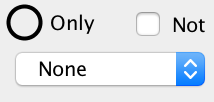
\includegraphics[width=1.25in]{constrain.png}}}
\vspace{-2em}
\caption{Constraints}
\vspace{-1em}
\label{constraintfacility}
\end{wrapfigure}

Some modules are outfitted with {\bf Constraints}: for example the {\bf Filter} module has a jack called {\it Only}, a checkbox called {\it Not}, and an unlabelled combobox (presently set to ``None'').  The constraints facility allows you to constrain which partials are being modified by the module and which are just passed through unchanged. 

\enlargethispage{1em}

\subsection{Partials Displays and Oscilloscopes}

\begin{wrapfigure}{r}{3in}
\vspace{-1em}
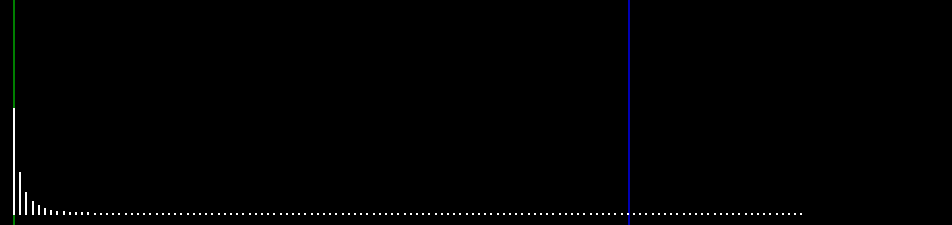
\includegraphics[width=3in]{display}
\caption{A Partials Display.  Note the partials to the right of the blue line.  These are beyond the Nyquist limit and are not audible.}
\label{display}
\end{wrapfigure}

There are four partials displays and oscilloscopes above the modules in the Rack.  The left partials display will show the partials of anything connected to the {\it A (Audio)} jack in {\bf Out}, that is, the partials being played as a sound.  The right display will show the partials of anything connected to the {\it B (Aux)} jack.  You can use this display as an auxiliary display.

Figure~\ref{display} shows a typical partials display.  Note that the display has a green vertical line: this indicates the position where the fundamental would be if it was exactly \(1\times f\) frequency: typically this marks the fundamental.  There may also be a blue line: this indicates where the Nyquist frequency cutoff is. Partials to the right of this line are not included in the final sound, and appear light gray on the display.  If you're confused, review the discussion of harmonics in Section~\ref{additivesynthesis}.  When a partial is 0.0 amplitude or higher than 1.0 amplitude, it turns red.

If you hover over a display with your mouse pointer, the display will highlight the nearest partial in orange, and it'll display some text, in the form:\\
\\
\begin{tabular}{@{\hspace{1in}}r}
Partial {\it partial}  Amp: {\it amp}  Freq: {\it absolute-freq} ({\it relative-freq})\\
Mouse  Amp: {\it amp}  Freq: {\it absolute-freq} ({\it relative-freq})\\
\end{tabular}\\

What this is saying is that the nearest partial to the mouse pointer (the one in orange) is partial number {\it partial}, and it has a given amplitude and relative frequency (where the fundamental would have frequency 1.0).  Multiplied against the current note pitch gives the provided absolute frequency.  Moreover, the mouse pointer is currently pointing to a spot which would be a certain amplitude, relative frequency, and absolute frequency as well.


\paragraph{Optional Display Features}
By default, partial frequencies are displayed linearly.  You can change this to a logarithmic plot by choosing {\bf Log-Axis Display} in the {\bf Options} menu.  There are two scaling options as well.  You can instruct Flow to provide enough room to display up to some \(N\) number of harmonics to the right of the fundamental by choosing the appropriate value under {\bf Max Displayed Harmonic} in the {\bf Options} menu.  The default is 150. If you're doing a logarithmic plot (this won't affect a linear display), you can also select how much room should be provided to the left of the fundamental by selecting {\bf Min Displayed Harmonic} from the {\bf Options} menu.  The default is 1/16.

Displays can also be set to {\it Waterfall Mode}, where the partials become dots (brighter dots are higher amplitude) and scroll by in time.  To try this out, choose {\bf Waterfall Display} in the {\bf Options} menu.  Finally, you can hide (or display) the displays with the menu option {\it Show Displays}: hiding the displays uses less computer power.

\begin{wrapfigure}{r}{1in}
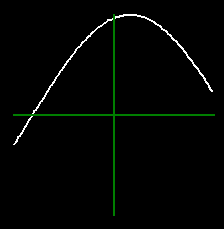
\includegraphics[height=1in]{oscilloscope}
\caption{An\newline Oscilloscope}
\vspace{-1em}
\label{oscilloscope}
\end{wrapfigure}

\paragraph{Oscilloscopes}
You might also find the oscilloscopes handy to understand what a modulation signal looks like.  The left oscilloscope shows the modulation signal of anything connected to the {\it 1 (Scope)} jack in {\bf Out}.  Notice for example, that in Figure~\ref{simplepatch}, the LFO is wired up to modulate the {\it 1 (Scope)} jack: this will cause it to be displayed in the left oscilloscope display.  Similarly, the right oscilloscope shows the modulation signal of anything connected to the {\it 2 (Aux)} jack.  Oscilloscopes have axes (the horizontal axis passes through the 0.5 position).  These axes change colors from blue to green (or from green to blue) any time the modulation triggers.  Oscilloscopes don't currently display any text when you hover over them.  Maybe they should!

A warning about oscilloscopes: like displays, they show the data of the most recently pressed note.  This can be confusing if (for example) you're using an LFO.  You've just reset the LFO with a note-on, but instead of resetting from its current position, it magically jumps to something much higher and resets from there.  This is because the voice being allocated for your note has its LFO at that position at the moment, {\it not the voice you've just been watching}, and the oscilloscope suddenly jumped to it.

\subsection{Playing a Patch}
\label{playingapatch}

\begin{wrapfigure}{r}{1.5in}
\vspace{-1em}
\includegraphics[width=1.5in]{Simple}
\caption{Playing a Sawtooth}
\vspace{-1em}
\label{simple}
\end{wrapfigure}

In order to hear a sound you need to first specify your {\bf Audio Device} from the window which pops up when you select {\bf MIDI and Audio Options} from the {\bf Options} menu.  I suggest setting it to your computer's speaker.

Now, if you directly connect a partials source ({\bf Sawtooth}, say) to the {\bf A (Audio)} input of your {\bf Out} module, it'll start playing.  In fact, {\bf all voices} might start playing: there's nothing to stop them!  It won't sound good.   At this point you're just testing your patch and may want to hear just a single voice.  To do this, select the menu option {\bf Monophonic} in the {\bf Play} menu.  The word "(Mono") will appear in the {\bf Out} module.

You might also choose {\bf Monophonic} if you'd like a monophonic synth.  Flow does {\it last note priority}, meaning that if, while playing monophonically, you hold down note A, then hold down note B, then hold down note C, then let go of C, then B will begin to sound, and if you let go of B, then A will begin to sound.

Ultimately you'll probably set things up with a {\bf VCA} (see the last entry in Section~\ref{unitshapers}) modulated by an {\bf Envelope} (typically a {\bf DADSR Envelope}: see Section~\ref{modsources}) which won't play the sound unless a key is pressed.  That way different voices are played when you play different keys.  At that point you'll want to uncheck {\bf Monophonic} so you can play more than one voice.

So how do you play a using keyboard?  You attach it to {\name} by selecting {\bf MIDI and Audio Preferences} from the {\bf Options} menu, then choosing the appropriate {\bf MIDI Device} and {\bf MIDI Channel}.  You'll notice an {\bf Auxillary MIDI Device} as an option: this lets you connect two MIDI devices to Flow.  It's not useful to use this unless you're in multitimbral mode (discussed in Section~\ref{multitimbral}).

If Flow is playing too loudly its sound will {\bf clip}. The title bar of the {\bf Out} module will briefly turn yellow and say ``Clip''.  You may also hear an audible buzz or click.  To prevent this in the future, you can turn down the sound's {\bf Gain} (in the {\bf Out module}).  You can also change the {\bf Master Gain} in the {\bf MIDI and Audio Preferences}, but this is better reserved for multitimbral mode instead.

\subsubsection{Using MPE}

To set up a MIDI Polyphonic Expression (MPE) device, go to {\bf MIDI and Audio Preferences} in the {\bf Play} menu, and change the MIDI Channel to either the MPE Lower Zone or the MPE Upper Zone, as determined by your MPE Controller.  You can then specify the number of MPE channels in the Zone.  {\name} also responds to an MPE Configuration Message (or MCM) sent over MIDI from your controller.

MPE devices are often designed to link certain behaviors to attack velocity, pitch bend, aftertouch, CC 74, and release velocity.  All of these are accessible via the {\bf MIDI In} module.  However, pitch bend and attack velocity also do specific things in Flow.  If you wanted Flow to respond in some {\it non-bend} way when you perform the bend behavior on a Roli Seaboard (say), you need a way to disable bend.  To do this, you can deselect {\bf Responds to Bend} in the {\bf Play} menu.  Similarly, you can disable {\bf Velocity Sensitive} in the {\bf Play} menu.  The Bend and Attack Velocity signals still will be sent to the MIDI In module, where you can tap into them to make your patch do what you like.

\subsection{Erasing, Loading, and Saving Patches}

You can clear the Rack to prepare for a new patch by choosing {\bf New Patch} from the {\bf File} menu.  Once you have created and tested your patch masterpiece, you can save it with {\bf Save Patch As...}.  You'll be prompted to give the patch a name, and then save it as a file.   You can resave your patch at any time with {\bf Save Patch}.  Later on, you can load a patch again with {\bf Load Patch...}\footnote{If you're launching Flow from the command line, you can have it open a patch like this:\hspace{\fill} {\tt java flow.Flow \textit{patchname.flow}}}

When you save a patch, if you have not already named the patch, the name of the patch will be set to the filename (minus its extension).  Thus if you save it to a file called {\it Foo.patch}, then the patch will be named {\it Foo}.  Once a file has been named\,---\,either after your first save, because you named it by choosing {\it Name Patch...} in the {\it Play} menu\,---\, its name won't change again even if you save it under a different file name.  To rename the patch, just select {\it Name Patch...} again.

There's only one Rack: you can't create or load multiple patches at a time.  If you load a patch, or clear it, the previous one will be deleted.

\subsubsection{Macros}
\label{aboutmacros}

One of the particularly interesting features of {\name} is its ability to load a saved patch as a {\bf Macro}.  A Macro encapsulates the patch and allows you to use it as a module in a larger patch.  Macro modules appear with green title bars and are named the name of the patch.

A patch is most useful as a Macro if it's been wired up to send and receive modulation and partials through its module.  To do this, you'll need to prepare the patch first.  See Section~\ref{creatingmacros} for an extensive discussion of the process.

\subsubsection{Naming Patches}

Patches have four pieces of auxiliary text information stored in them: a {\it patch name}, a {\it patch author}, a {\it patch date}, a {\it patch version}, and some {\it patch info}.  You can put whatever you like in these four text boxes: just choose {\bf Patch Info...} from the {\bf Play} menu.

A patch doesn't need to have an author, date, version, or info: but it ought to have a name.  This is because if you load a patch as a Macro, the Macro's module will be titled with the patch name.  If you save a patch that has no name (yet), {\name} will set the patch name to the filename (minus the extension).

\subsection{Connecting to a Digital Audio Workstation}
\label{connecting}

The primary challenge to connecting Flow to a DAW is that both Flow and your DAW are designed to connect to {\it MIDI Devices} and {\it Audio Devices}, yet neither of them {\it is} a MIDI or Audio Device!  Thus neither of them can connect to each other!  This is a stupid mistake in how MIDI and Audio routing is implemented in operating systems, but there you have it.

To get Flow and a DAW to send MIDI and Audio data to each other, you need to create a {\it MIDI Loopback} device and an {\it Audio Loopback} device.  A Loopback device is a tunnel which presents itself as a device at each end: by connecting an application at one end and an application at the other end, each thinks it's talking to a device, but in fact they are talking to each other.

The problem with loopback devices is that they are slow: they introduce a great deal of latency both in MIDI and audio.  This is the biggest problem with using Flow with a DAW.  Flow has certain features which help mitigate this.  

\paragraph{Routing MIDI from a Digital Audio Workstation}

\begin{wrapfigure}{r}{3in}
\vspace{-2em}
\begin{center}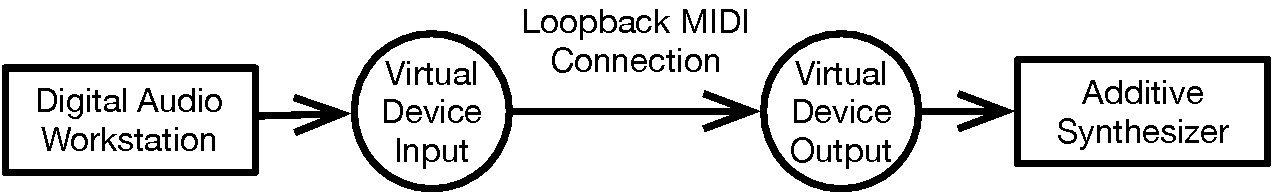
\includegraphics[width=3in]{loopbackmidi}\end{center}
\vspace{-1em}
\caption{A MIDI loopback connecting a Digital Audio Workstation to {\name}.  Compare to Figure~\ref{loopbackaudio}.}\label{loopbackmidi}
\end{wrapfigure}

To enable your DAW to send MIDI to Flow, you need to make a {\it MIDI loopback}.  This is where you create two {\it virtual devices} which are connected to one another.  {\name} and your DAW can both see these devices.  Consider Figure~\ref{loopbackmidi}.  If your DAW outputs to Virtual Device X (say) and {\name} is set up to {\it input} from Virtual Device X, then it will receive what the DAW outputs.

Making a MIDI loopback device varies depending on your operating system:

\begin{itemize}
\item {\bf On the Mac}\quad First, open the application \textsf{/Applications/Utilities/Audio MIDI Setup}.  Next, click on the ``IAC Driver'' icon to open the ``IAC Driver Properties'' window.  Add a new port, named whatever you like (I named mine ``From Ableton'').  Check the box ``Device is Online''.  This new port will appear to your DAW and to {\name} as the loopback device.

\item {\bf On Windows}\quad There is no way to do this in Windows directly: instead you'll need to run a program which provides this service.  Programs include {\sf loopMIDI},  {\sf loopBe1}, MIDIOx's {\sf MidiYoke}, and so on.  Googling for ``loopback MIDI Windows'' will get you there. 

\item {\bf On Linux}\quad In most flavors of Linux, to get virtual devices running you'll first need to type the command \hbox{\tt sudo modprobe snd-virmidi} and then type in your password.  \quad If you're using something like Gentoo or any other distro that does not come with this kernel module, you'll need to custom compile your kernel to get it. 

This procedure will create a bunch of of virtual devices with names like {\tt VirMIDI [hw:2,0,0]} or {\tt VirMIDI [hw:2,1,8]}.  Select a device whose third number is 0 (such as {\tt VirMIDI [hw:2,0,0]} or {\tt VirMIDI [hw:3,1,0]}, but not {\tt VirMIDI [hw:2,1,1]}).  Have the DAW send to this device and have {\name} listen from the same device.
\end{itemize}

\paragraph{Routing Audio from a Digital Audio Workstation}

\begin{wrapfigure}{r}{3in}
\begin{center}\vspace{-2em}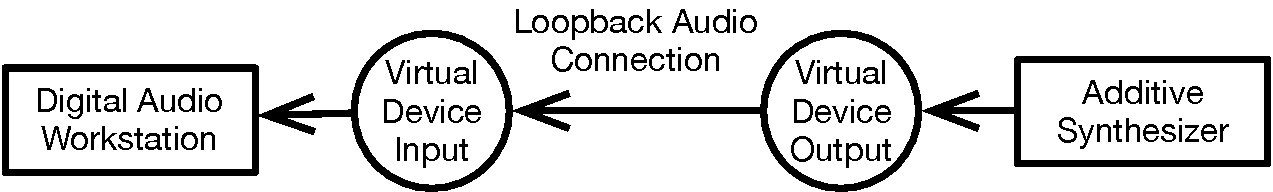
\includegraphics[width=3in]{loopbackaudio}\end{center}
\vspace{-1em}
\caption{An Audio loopback connecting {\name} to a Digital Audio Workstation.  Compare to Figure~\ref{loopbackmidi}.}\label{loopbackaudio}
\end{wrapfigure}

To send audio from Flow to your DAW to be recorded, you'll need a loopback device for audio similar to the one for MIDI.   Once again how you'd make an Audio Loopback device depends on your operating system:

\begin{itemize}
\item {\bf On the Mac}\quad Unlike for MIDI, there's no built-in audio loopback facility on the Mac.  You'll need to install a program which does audio loopbacks.  There is an open-source driver called {\it SoundFlower}\footnote{https:/\!/github.com/mattingalls/Soundflower/releases/\qquad Note that the GUI installer fails on High Sierra even if you have given permission per the instructions on the website.  But installing via the Terminal seems to work.  Do the following:

\begin{enumerate}
\item Unpack the {\tt Soundflower-2.0b2.dmg} disk image.
\item In the terminal, type:
\begin{tabbing}
~\hspace{5em}{\tt cd /Volumes/Soundflower-2.0b2}\hspace{2in}\= {\it Then press RETURN}\\
~\hspace{5em}{\tt sudo installer -pkg Soundflower.pkg -target /}\>{\it Then press RETURN}
\end{tabbing}
\item Enter your password and press RETURN.
\item When you're told that this has failed, go to ``Security and Privacy'' in System Preferences, and permit the software to load.  You may need to click "Allow...", then select ``MATT INGALLS'' (he's the developer) in the list and approve it.  Then do steps 2 and 3 again.
\item Wait a long time.  It takes quite a while to install for no good reason.
\item At this point, SoundFlower 2ch and 64ch will appear as audio devices.  You want SoundFlower 2ch.  You can configure it further in Audio MIDI Setup if you like, or just use it straight.
\end{enumerate}
}
which seems to work fine though with high latency.  If you'd like support and a better user experience, I recommend the commercial product {\it Loopback} by Rogue Amoeba.\footnote{https:/\!/rogueamoeba.com/loopback/}  It works very well, and if you're poor you can try it in unfettered trial mode for about 20 minutes, quit it, and start it again for another 20, etc.   There are also various tools built around the {\it Jack} framework: but Jack seems to be break all Java Audio applications: you won't be able to run {\name} at all after installing Jack.  And furthermore, Jack's {\it uninstaller} is seriously broken: it doesn't remove the necessary files and you'll be permanently unable to run anything that needs Java Audio (including {\name}).  {\color{red}\bf Do not install Jack on OS X.}  You will regret it.\footnote{In fact, after I reported this, Jack's administrators seem to be leaning towards eliminating Jack on OS X entirely.  Oh well.  If you screwed up and installed Jack on OS X, the following URL contains a list of all the files you'll need to remove manually (as administrator): https:/\!/github.com/jackaudio/jack2/issues/379}

\end{itemize}

\begin{itemize}
\item {\bf On Windows}\quad I can't help you here.  I'm sure there's many ways to do this, but I don't know them.

\item {\bf On Linux}\quad You'll want to use Jack 2 and Cadence. A good solution with minimal friction is to enable the ALSA and Pulseaudio bridges from within the Cadence GUI. Set the buffer size for your sound card in Cadence to something small, like 128 samples (ideally, the smallest you can get it without glitches): this allows you to minimize the application buffer size, reducing latency. After running Cadence and starting the jack daemon, run flow and set the sound output to the jack bridge in Pulseaudio via Pavucontrol (or an equivalent audio configurator). This will allow you to route audio from Pulseaudio into jack, which will most likely be able to interface with your DAW and other audio applications.

\end{itemize}


\begin{figure}[t]
\begin{center}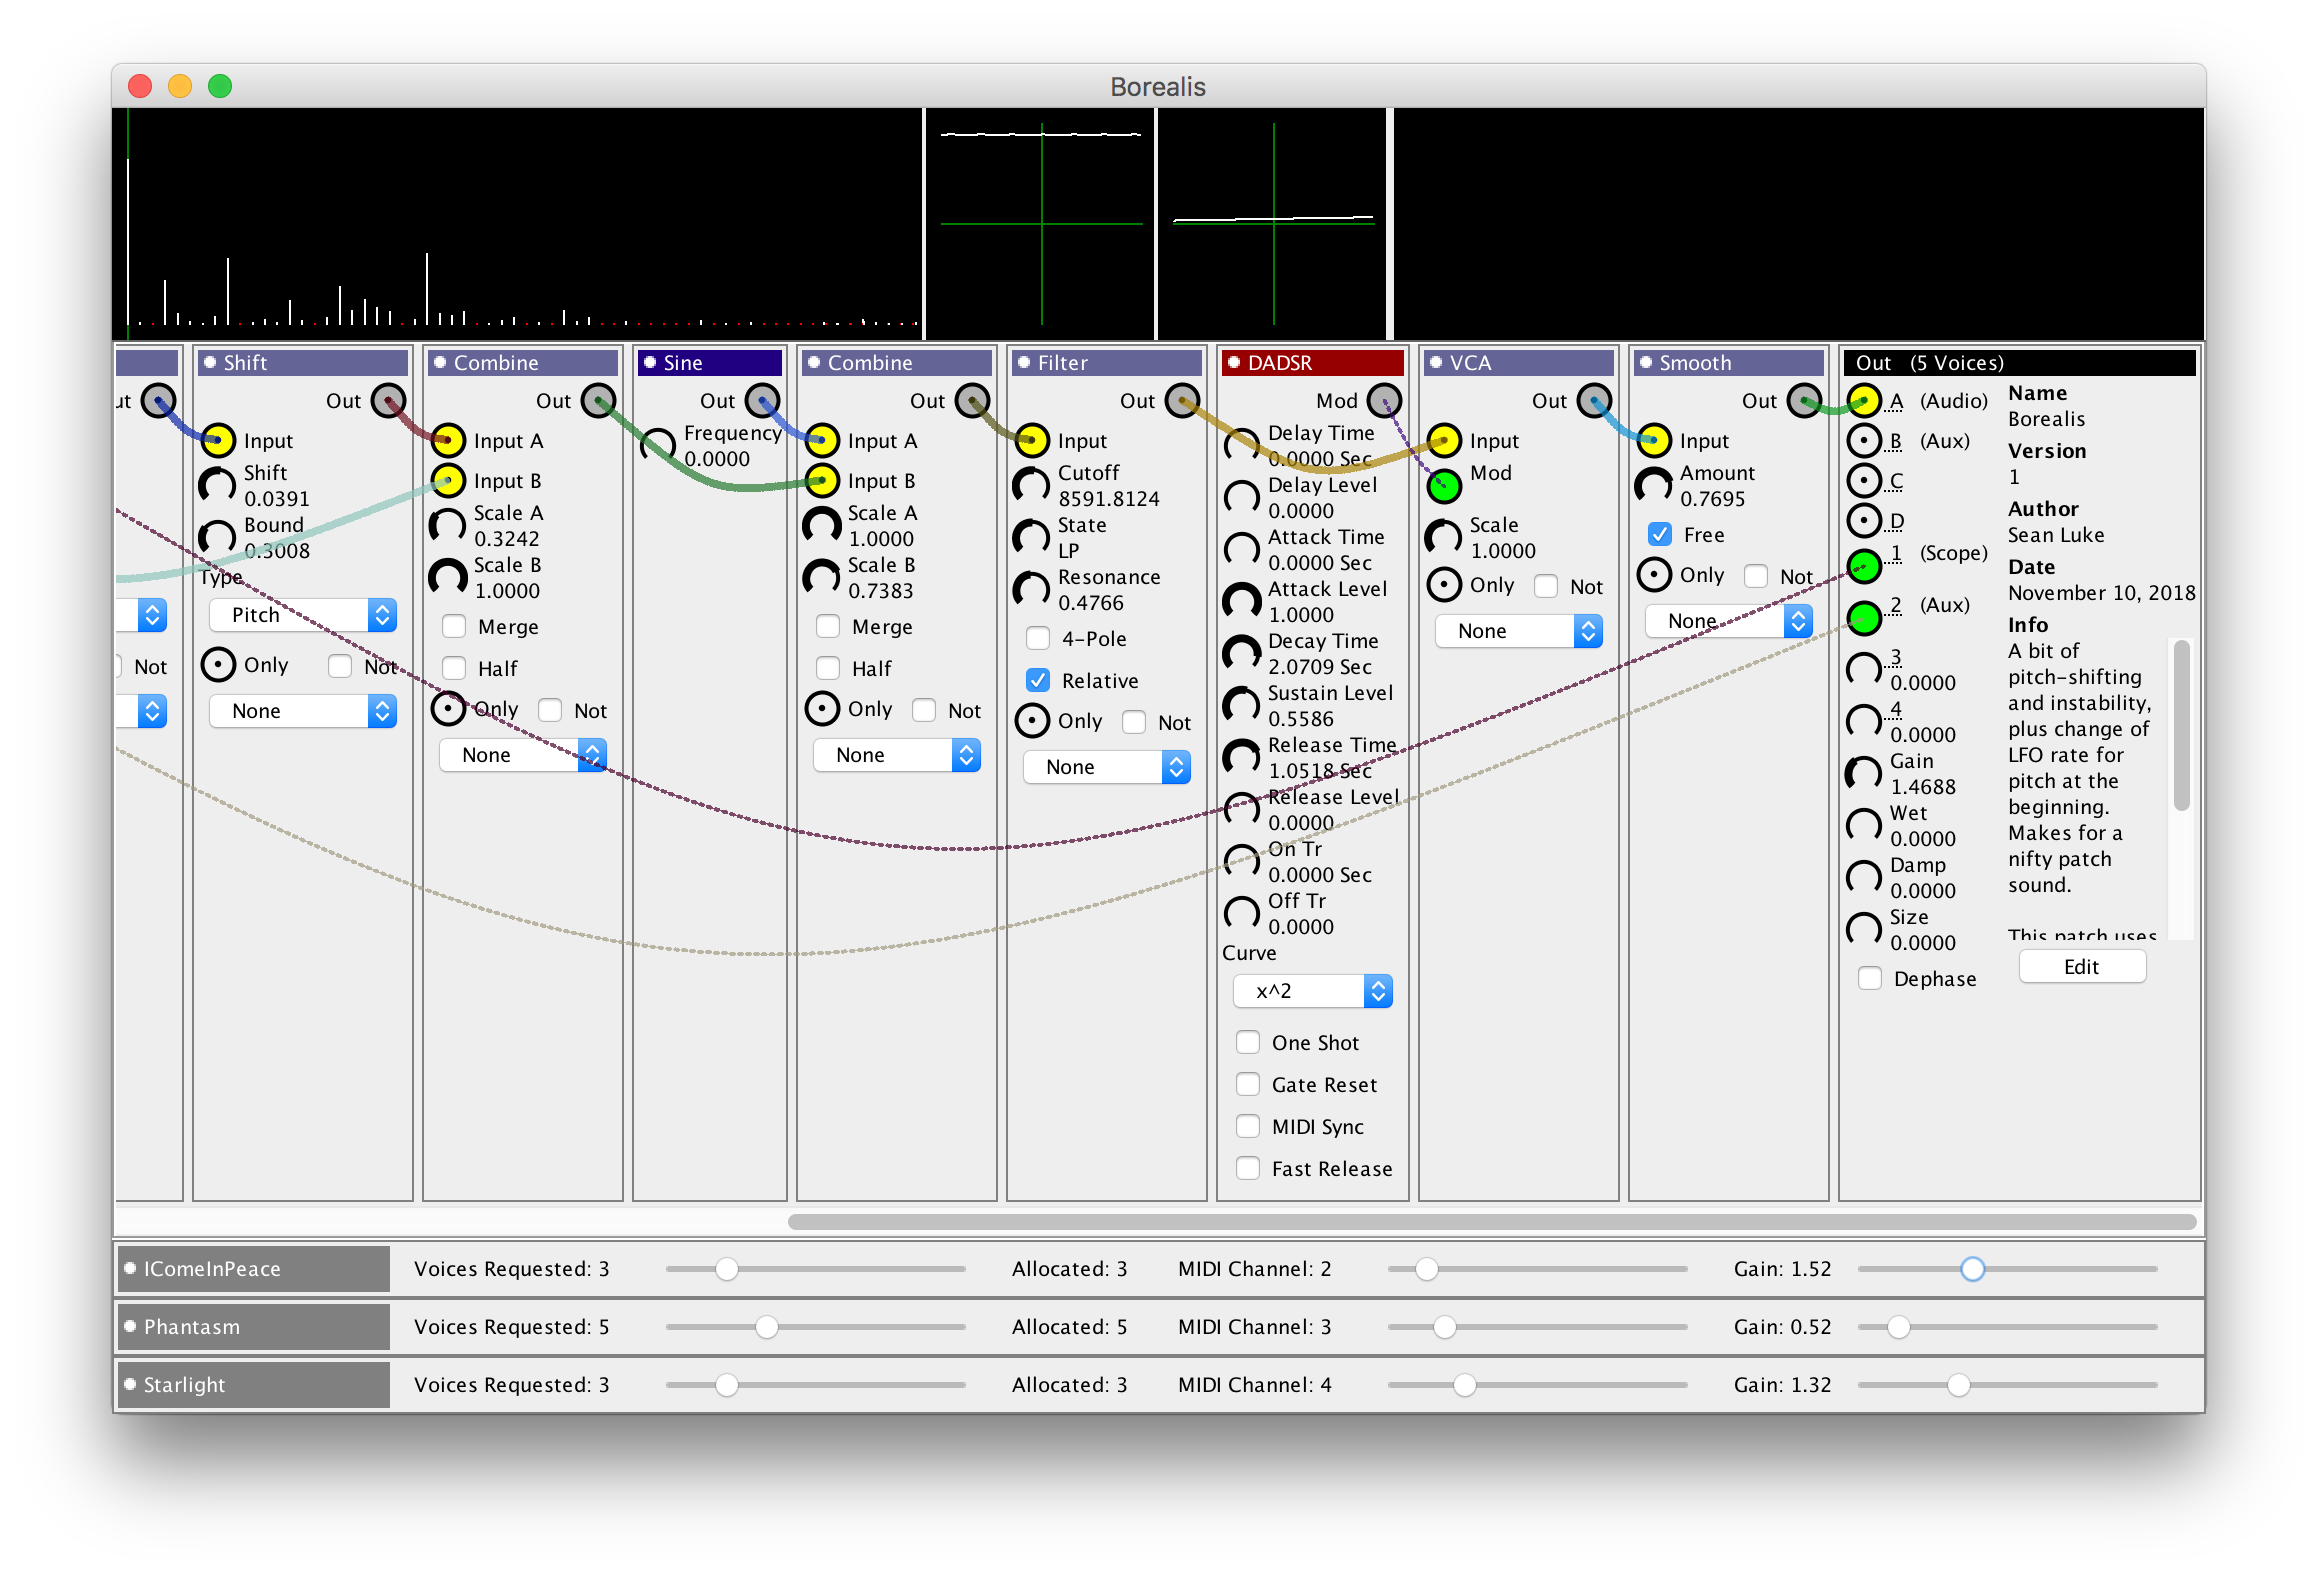
\includegraphics[width=6.5in]{subpatches}\end{center}
\vspace{-3em}
\caption{Primary patch and three subpatches.}
\label{subpatches}
\end{figure}

\subsubsection{Multitimbral Patches}
\label{multitimbral}

Flow can be set up to play more than one patch at a time. This is particularly useful because Flow is a very computationally costly: if you have attached Flow to a DAW and you want to play more than one Flow patch through the DAW, you'd probably rather not run multiple copies of the application, each tuned with a small number of voices.

In most synthesizers, a multitimbral patch is different from a ``single'' (one-sound) patch.  In synthesizers like this, you'd make a bunch of single patches, then make one multitimbral patch which references all of them.  Flow's multitmbral patch model is different.  In Flow, you load a single patch, which we'll call the {\it primary patch}, then you attach one or more additional single patches to it as {\it subpatches}.  You can save this combined bundle of patches out to a standard file and load it again.  An example of a primary patch and three subpatches is shown in Figure~\ref{subpatches}.

Subpatches are added to the primary patch by choosing {\bf Load Subpatch...} in the {\bf File} menu.  Only the primary patch can be edited: the subpatches will appear as thin rows beneath its modules.  For each subpatch you can make the following settings:

\begin{itemize}
\item {\bf Voices Requested}\quad Here you stipulate how many voices you'd like to allocate to this subpatch.  Voices allocated to a subpatch are taken out of voices available to the main patch. 

\item {\bf Voices Allocated}\quad Obviously not every subpatch can have a maximal number of voices.  Here you can see how many voices were {\it actually} allocated.  The allocation strategy is simple: for each subpatch from top to bottom, Flow attempts to give that subpatch every voice it asked for.  Flow must reserve at least one voice for the main patch, so there are at most 15 voices available to distribute (or whatever the polyphony was that you specified in your tuning parameters).  If Flow runs out of voices, a subpatch may get fewer voices than it asked for, and later subpatches may get no voices at all.  

One confusing situation arises when you have selected {\it Monophonic} from the {\it Play} menu.  Here Flow only uses a single voice, and that voice must go to the primary patch, so the subpatches will all have zero voices.  To make this situation clear, the subpatches will show {\bf [M]} (for ``monophonic'') for the number of voices allocated, and  ``(Mono)'' will appear in the {\bf Out} module of the primary patch.

\item {\bf MIDI Channel}\quad This specifies which MIDI channel is used by the subpatch (or, if no MIDI channel, ``Off'').  If multiple subpatches request the same MIDI Channel, the earlier (higher) one will prevail.    Subpatches also get MIDI channel priority over the primary patch, so if a subpatch and the primary patch are using the same MIDI channel, the subpatch gets it.

This has interesting implications when the primary patch is set to ``Any Channel'', ``MPE Lower Zone'', or ``MPE Upper Zone''.  Let's start with ``Any Channel''.  If your primary patch is set to this, then it responds to any channel {\it except} for the ones allocated to the subpatches.

MPE is more complicated.  Recall that if you are using MPE, then you also specify the number of MPE channels.  If you have chosen MPE Lower Zone with \(n\) channels, then normally the patch would be allocated MIDI channel 1 for its {\it MPE Global Channel} and channels \(2\ ...\ n + 1\) for the requested MIDI channels.  However if a subpatch has allocated one of those channels, it will take it from the primary patch.  This will disrupt MPE.

Thus if you have chosen MPE Upper Zone with \(n\) channels, you want your subpatches to request channels somewhere in the range \(n+2\ ...\ 16\).  For example, if you have 3 subpatches, you might set up MPE Upper Zone with \(n=12\) (so MPE needs channels \(1\ ...\ 13\)), and then use channels 14, 15, and 16 for the subpatches.

If you have instead chosen the MPE Upper Zone with \(n\) channels, then the MPE Global Channel is 16 and the MPE channels go down from there, that is, they're assigned to \(16 - n\ ...\ 15\). Once again, you want your subpatches to stay out of this region, so you'd assign to subpatches channels in the region \(1\ ...\ 16 - n - 1\).  For example, if you have 3 subpatches, you might once again set up MPE Upper Zone with \(n=12\) (so MPE needs channels \(4\ ...\ 16\)), and then use channels 1, 2, and 3 for the subpatches.

Subpatches cannot use MPE, nor can they be assigned to ``Any Channel''.  Only the primary patch can.

\item {\bf MIDI Note}\quad You can restrict a sound to only respond to a given note: any other notes on the MIDI channel will be passed on to later sounds.

\item {\bf Gain}\quad This sets the overall volume of the subpatch in the final mix.  This is exactly the same as the {\it Gain} knob on the {\bf Out} module of the primary patch, mentioned earlier in Section~\ref{playingapatch}.  And in fact, the Gain knob can be modulated: if your subpatch was originally modulating its Gain knob before you loaded it as a subpatch, it will {\it continue} to modulate the gain, overriding the setting you make here.  In general it's probably not  wise to modulate the Gain knob.

If you want to change the overall gain of the primary patch and all the subpatches, you can do this by changing the {\it Master Gain} option in {\bf MIDI and Audio Preferences}.   Note that Master Gain is not saved with patches and is reset when you restart Flow.

\item {\bf Rename}\quad You can rename the subpatch name.
\end{itemize}

Flow mixes the primary patch and subpatch voices as follows: each voice is amplified according to its the gain of its patch or subpatch, and then the voices are added together.  Finally all the voices are pushed through the reverb.  This means that {\bf reverb is global}: the settings you make in the primary patch will affect all voices, even ones in subpatches.  We may change that in the future.

You can remove a subpatch by clicking on its close box, just like removing a module.  You can also drag subpatches to reorder them relative to one another, just like modules.

\paragraph{Primary Patch Parameter Display}  Subpatches take priority over the primary patch both in allocated voices and MIDI channels, so how you set them seriously affects the primary patch's resources.  You can see what those resources are by looking at the title bar of the {\bf Out} module:

\begin{itemize}
\item {\bf Voices}\quad  If the title just says {\it Out}, then it has full voices. Otherwise it'll say something like {\it Out (13 Voices)}.
\item {\bf Monophonic}\quad  If you are playing in monophonic mode, the Primary patch gets the one and only voice.  In this case, the title will say {\it Out (Mono)}.
\item {\bf MIDI Channel}\quad  If you have any subpatches, the title will display the MIDI channel of the primary patch.  For example, if the channel is 13, the title will say something like {\it M13}.  If another subpatch has {\it also} chosen channel 13, then the title will say {\it M13?}.  Whether the subpatch has fully overridden the primary patch depends on whether the subpatch is restricted to a single MIDI Note (and it's different from the primary patch of course).
\item {\bf MIDI Note}\quad  Speaking of the MIDI note: normally you can't set the MIDI note in a primary patch\,---\,however if you set it in a subpatch, then swap the subpatch to the primary patch, then it will have a MIDI note (mostly under the assumption that you're doing this temporarily and will swap it back).  In this case, the note will be displayed, something like {\it Ab2}.
\end{itemize}

\paragraph{Changing Subpatch Order}

As mentioned before, the order of the subpatches affects which patches get allocated voices and priority over MIDI channels.  You change this order by dragging the titlebar of a subpatch and dropping it before or after another subpatch.

\paragraph{Swapping a Subpatch with the Primary Patch}

If you drag the titlebar of a subpatch clear into the region of the {\it primary patch}, it will {\bf swap} the subpatch with the primary patch.  Flow will preserve reverb from the previous patch.  This is useful for making a subpatch the the Primary Patch temporarily in order to tweak it.

Swapping the MIDI channel come with some caveats.  First, only the Primary patch can perform MPE: so if you are swapping a primary patch that uses MPE, when it becomes a subpatch its MIDI channel will become ``No Channel''.  Similarly, only subpatches can have ``No Channel'' as a MIDI channel option,\footnote{This may change in the future.} so if one of them is swapped to a primary path, its MIDI channel will change to ``All Channels''.

Another thing you need to watch out for is swapping the Primary patch whose Gain is under the control of a modulation such as an LFO.  When it becomes a subpatch, the subpatch's Gain slider will be set to 0 (and it won't work anyway).  In short: don't control Gain from a modulation.

You can also swap a subpatch with  swap while holding down the Control key (on the Mac, you can also hold the Option key).\footnote{Yes, I know this is the behavior for ``copying'' while drag and drop, and in fact you'll get a copy icon.  But there's no ``alternative drag'' option in Java, so I had to make do.}  This will swap the two patches but the MIDI channel, MIDI Note, and Number of Requested Sounds won't change.  Why would you want to do this?  If you are auditioning a bunch of different sounds, you may have them lined up as subpatches and are dragging them into the primary patch to hear them play a given part (which has its own MIDI channel).

\paragraph{Loading, Clearing, and Saving the Primary Patch}  Obviously you could clear the primary patch or load a new one by choosing {\it Load Patch...} or {\it New Patch} respectively, but this would clear out the subpatches as well.  If you just want to clear just the primary patch alone, choose {\it New Primary Patch}.  You'll be asked if you wanted to optionally {\it demote} the primary patch, that is, to turn it into a subpatch rather than eliminate it. 

Similarly, if you choose {\it Load Primary Patch...}, you will load a new primary patch, replacing the original, but keep the subpatches.  You will likewise be asked if you would like to optionally {\it demote} the primary patch just as before.  If you'd like to save the primary patch to a file (but not its subpatches), you can choose {\it Export Primary Patch...}  This sometimes happens when you've modified a subpatch in a multitimbral setting and would like to keep it: swap it to the primary patch, export it, then swap back.

\subsubsection{Digital Audio Workstation Integration Strategies}

Here's a common scenario.  You have so far recorded MIDI for several Flow tracks in your DAW, and you're currently recording MIDI for a new track while playing the old ones.  This new track is connected to Flow's Primary Patch, while the several old tracks are connected to subpatches.  When you have finished recording the new track, you load a new patch into Flow's Primary Patch, demoting the current Primary Patch to a subpatch, and you begin anew.

To get this scenario working, you assign each Flow subpatch a unique MIDI channel.  The Primary patch also gets its own MIDI channel.  Your keyboard is connected to the DAW's recording track, and the DAW is rerouting its MIDI data to the primary patch in Flow.  Flow's sound output is connected to the DAW in anticipation of eventually recording the audio: for now the DAW is just routing it to the speakers.

\paragraph{Latency} There is a big problem with this scenaro: high latency.  Your MIDI keyboard is routed to the DAW, which is then {\it rerouting} it to Flow, which is then sending audio to the DAW, which is then {\it rerouting} the audio to your speakers.

We can reduce the MIDI latency by eliminating the rerouting: the DAW doesn't reroute the keyboard to Flow, but only records it into the track.  Instead, we set up the keyboard as a {\it second MIDI device} in Flow: it's going directly to Flow's Primary patch.  The DAW is also sending MIDI to Flow (for the subpatches).  To do this, you can set the keyboard as the {\bf Aux MIDI Device} in the {\bf MIDI and Audio Options} window.  Make sure that the DAW isn't routing the keyboard to Flow as well or you'll get two copies of the same MIDI data.

The best way to reduce the Audio latency is to not send audio to the DAW until you absolutely have to (to record an audio track).  Instead, just have Flow play directly to your speakers.

\paragraph{Computational Cost} Flow uses a lot of CPU.   {\it A lot of CPU.}   Your objective is to eek out as many voices as possible to make your song before it begins to glitch.  I can usually get 20--24 voices on my laptop.  How is this done?

\begin{itemize}
\item Turn off Flow's display.  That saves a lot.
\item For each subpatch, reduce the voices requested to the minimum number needed before you hear the artifacts of voice stealing. 
\item If necessary, temporarily reduce the number of partials being used while recording and editing the MIDI in tracks.  Then bring the partials up to (say) 256 for the final audio recording.  This is an extreme measure but it works, especially in combination with...
\item You can significantly increase the audio buffer size in the final recording, which will reduce glitching by quite a lot even with 256 partials and a maxed-out voice count: the downside is heavily increased latency, but that wouldn't matter for the final audio recording and can be shifted in post.
\item Keep in mind that some patches are much more costly per-voice than others.  Keep their voice counts minimized.
\item Shut off other applications: especially web browsers and other CPU-hungry stuff.
\end{itemize}

\paragraph{Compressing Tracks} I am cheap and don't own a full-featured copy of Abelton: I just have Ableton Live Lite.  The problem with this is that I am restricted to 8 tracks total, including the audio track (I record multiple MIDI tracks, then play them together with subpatches and record a final audio track).  This means that I can have at most 7 MIDI channels going into Flow.  How then can I play (say) 12 different sounds?

It's often the case that many of my sounds are percussion.  Percussion sounds are typically played with a single note each\,---\,indeed it doesn't matter what the note is because I use the {\bf Fix} module (Section~\ref{specialmodules}) to force them to play at a certain pitch anyway.  For this reason, I often assign each percussion sound to a certain note: the bass kick to C4, the high hat to C5, etc., and have them all recorded like a drumset on a single track.

Flow can handle this without any difficulty: each percussion subpatch has the exact same MIDI channel, but is assigned a different   note via the subpatch's {\bf MIDI Note} restriction.  The kick gets assigned to C6 etc.\footnote{Note that Ableton's octaves go from -2 to 8 in old Yamaha tradition, while Flow's go from 0 to 10.  I just add 2 to convert to Flow.}  This lets me play multiple Flow percussion sounds from a single track!

\paragraph{Master Gain} At the end of the day I can get my whole song to play without glitching, but it still clips here and there.  Rather than go through and adjust the gain of each subpatch separately, I just pull down the master gain (see the {\bf MIDI and Audio Options} window).     Note that Master Gain is not saved with patches and is reset when you restart Flow.

\bump

\section{The Modules}

The Modules are divided into five categories:

\begin{itemize}
\item {\bf Modulation Sources}\quad Are meant to be sources of modulation information.  Example: a low frequency oscillator (LFO).
\item {\bf Modulation Shapers}\quad Are meant to modify modulation information.  Example: a module which takes an incoming signal and does a Sample and Hold on it.
\item {\bf Partials Sources}\quad Are meant to be sources of, well, partials.  Example: a sawtooth wave.
\item {\bf Partials Shapers}\quad Are meant to modify partials, producing new ones.  Example: a low pass filter.
\item {\bf Special}\quad Various system modules, such as In, Out, Choice, Fix, Note, and Macro.  Just because these are at the end doesn't mean they're not important (they're probably the {\it most} important!).
\end{itemize}

\subsection{Modulation Sources}
\label{modsources}

\begin{wrapfigure}{r}{3in}
\vspace{-1em}
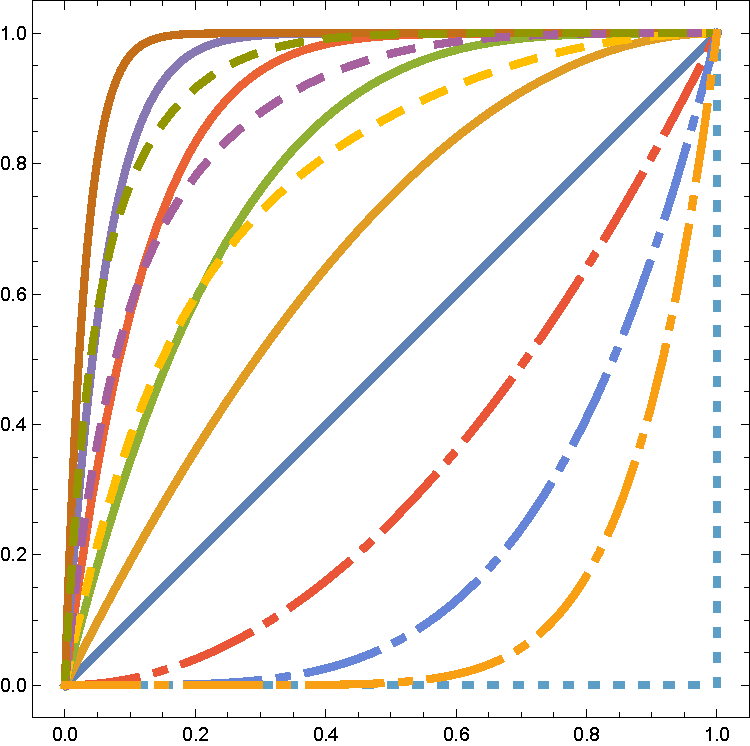
\includegraphics[height=1.5in]{CurveUp}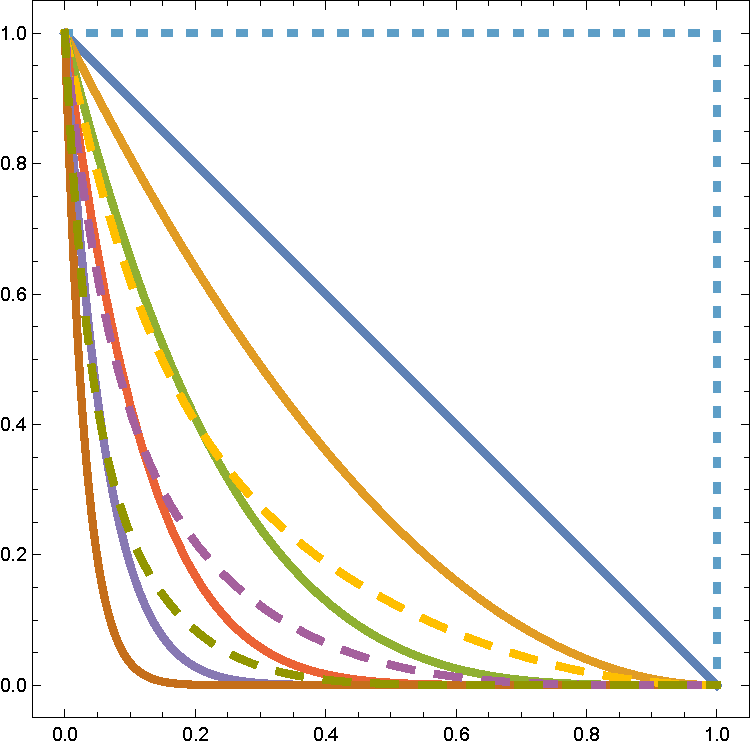
\includegraphics[height=1.5in]{CurveDown}
\caption{Envelope modulation curves, shown both in rising and falling scenarios.  Solid lines are (right to left) {\it Linear}, \(x^2\), \(x^4\), \(x^8\), \(x^{16}\), and \(x^{32}\).  Dotted lines are (right to left) \((x^2 + x^8)/2\),  \((x^4 + x^{16})/2\), and  \((x^8 + x^{32})/2\).  Not shown is {\it Step}, which stays put until the very end, at which time it suddenly jumps to the ultimate value. }
\label{curves}
\end{wrapfigure}

\paragraph{AHR}  A simple Attack-Hold-Release (or is you like Attack-Hold-Decay) envelope.  As you play a note, this envelope starts at the Start Level, ramps up to the Attack Level over the course of the Attack Time, then holds at that level for the Hold Time.  It then releases (decays) back to the Start Level over the Release Time.  If you let go of the key early, it immediately starts releasing for the given Release time (unless it's already releasing, in which case it just continues to do so).  AHR is much simpler than the DADSR envelope module, but it does have one feature that DADSR does not: you can specify the attack and release curves separately.  Curves are specified from linear to pseudo-exponential, plus ``Step'', which immediately steps to the next level.  Figure~\ref{curves} shows available curves.  The envelope can be one shot, meaning it continues until it is finished even if you have released.   The envelope triggers on completion of each of its stages.  You can request that the envelope sync to MIDI when the synthesizer is set to MIDI (otherwise it's based on time as usual).  If you double-click on any time dial, a pop-up menu will appear which lets you set various note speeds corresponding to playing at 120BPM.  If the MIDI clock is running, these note speeds will correspond to the MIDI clock's rate.

AHR can be configured to instead act as a {\it ramp} function: when a Note-On happens, the envelope restarts at the Start Level, then ramps to the Attack Level over the course of the Attack Time, and  {\it holds there indefinitely.}  A Note-Off simply stops the ramping and it holds wherever it stopped.  If the envelope is one-shot, then a Note-Off has no effect at all. 

The {\it On Tr} option restarts the envelope whenever it receives a trigger (as if a Note-On happened), and the {\it Off Tr} option starts the release stage whenever it receives a trigger (as if a Note-Off happened).  These are auxiliary triggers: don't use them to trigger on a note-on/note-off directly (as in from the MIDIIn module).  The envelope does that by default already.  Furthermore, if you connect to the On Tr port, then the envelope will {\it only} restart whenthen a trigger occurs: it will {\it not} restart on a Note On.  Similarly, if you connect to the Off Tr port, then the envelope will {\it only} release when a trigger occurs: it will {\it not} release on a Note Off.  See also {\bf DADSR} and {\bf Envelope}.

\paragraph{DADSR}  A standard Delay-Attack-Decay-Sustain-Release envelope.\footnote{Though in fact the ``Delay'' is really just a first-stage attack: it's only effectively a delay if its level is set to 0.  Indeed, if you treated it as an attack, and then set Attack's level to the same as Delay's level, then you'd have an``ADHSR'' (``H'' for ``Hold'', as in E-mu products and the Moog One.} You can select curves from linear to pseudo-exponential, plus ``Step'', which immediately steps to the next level.  Figure~\ref{curves} on page~\pageref{curves} shows available curves.  The envelope can be one shot (it doesn't stop at sustain), and it can be set to reset to 0 on a Gate (Note Down), as opposed to just starting from its current position.  The envelope triggers on completion of each of its stages.  You can request that the envelope sync to MIDI when the synthesizer is set to MIDI (otherwise it's based on time as usual).  Finally, {\it Fast Release} changes how release and Decay interact.  If Fast Release is true, then on Note Off, the envelope will start the release stage immediately; but if Fast Release is false (the default), then if you do a Note Off during the Delay stage, the Delay stage will be completed fully before the release starts.  No other stages are affected: for example, if a Note Off occurs during Attack, release immediately starts no matter what.

If you double-click on any time dial, a pop-up menu will appear which lets you set various note speeds corresponding to playing at 120BPM.  If the MIDI clock is running, these note speeds will correspond to the MIDI clock's rate.

The {\it On Tr} option restarts the envelope whenever it receives a trigger (as if a Note-On happened), and the {\it Off Tr} option starts the release stage whenever it receives a trigger (as if a Note-Off happened).  These are auxiliary triggers: don't use them to trigger on a note-on/note-off directly (as in from the MIDIIn module).  The envelope does that by default already.  Furthermore, f you connect to the On Tr port, then the envelope will {\it only} restart when a trigger occurs: it will {\it not} restart on a Note On.  Similarly, if you connect to the Off Tr port, then the envelope will {\it only} release when a trigger occurs: it will {\it not} release on a Note Off.  See also {\bf AHR} and {\bf Envelope}.
 
\paragraph{Envelope}  An eight-stage envelope with looping.  The envelope has three stages prior to sustain, then three sustain stages, then two stages at release.  Each stage has a time to completion, and a level at which it will have reached when completed.  If the time is set to 0.0, then the stage is ignored entirely.\footnote{This means that if you attach modulation to your envelope time values, you might want to make sure your modulation doesn't quite hit 0.0, or things might not work exactly as expected.}  There is also a {\it Start} option which specifies the initial level.  The envelope triggers on completion of any of its stages.  You can select curves from linear to pseudo-exponential, plus ``Step'', which immediately steps to the next level.  Figure~\ref{curves} on page~\pageref{curves} shows available curves.  You can request that the envelope sync to MIDI when the synthesizer is set to MIDI (otherwise it's based on time as usual). 

The Envelope has several types.  {\it Sustain} works like a regular envelope: it works its way up through the final sustain state and then stays there, and if you do a note-off, it starts immediately on the first release state and continues from there.  {\it Sustain Loop} works like Sustain, but once the final sustain state has been completed, it loops back through the sustain states rather than staying at the last one.  {\it One Shot} works its way through all the states until  it has completed them, regardless of note off.  {\it Play Through} is like {\it One Shot}, except that it jumps to the first release stage on note-off; thus Play Though is like Sustain but without waiting at the last sustain stage.  {\it Loop w/Rel} (Loop with Release) loops through all the states over and over again, and stops looping on note-off.  {\it Loop} loops through all the states over and over again forever; but is reset on note-on like all other envelope types.
   
If you double-click on any time dial, a pop-up menu will appear which lets you set various note speeds corresponding to playing at 120BPM.  If the MIDI clock is running, these note speeds will correspond to the MIDI clock's rate.

The {\it On Tr} option restarts the envelope whenever it receives a trigger (as if a Note-On happened), and the {\it Off Tr} option starts the release stage whenever it receives a trigger (as if a Note-Off happened).  These are auxiliary triggers: don't use them to trigger on a note-on/note-off directly (as in from the MIDIIn module).  The envelope does that by default already.  Furthermore, if you connect to the On Tr port, then the envelope will {\it only} restart when a trigger occurs: it will {\it not} restart on a Note On.  Similarly, if you connect to the Off Tr port, then the envelope will {\it only} release when a trigger occurs: it will {\it not} release on a Note Off.   See also {\bf DADSR} and {\bf AHR}.

\paragraph{LFO}  A low-frequency oscillator with a rate and phase, a shift of its zero point vertically, and vertical scaling of the wave.   If you double-click on the rate dial, a pop-up menu will appear which lets you set various note speeds corresponding to playing at 120BPM.  If the MIDI clock is running, these note speeds will correspond to the MIDI clock's rate.

The oscillator can run free, you can invert the wave.    The LFO triggers on completion of one full wave, or one-half wave if {\bf Half Trigger} is set.  If {\it Init Trigger} is set, then the LFO also triggers on the start of the very first wave.  The waves can be sine, triangle, saw up, square, random, and random sample and hold.   You can request that the LFO sync to MIDI when the synthesizer is set to MIDI (otherwise it's based on time as usual).  And finally, you can indicate that the rate dial should be linear and not exponential (which is useful when modulating an LFO with another LFO).

Random works as follows: a random new target Y position is set and the LFO spends {\it rate} time to get there.  Once it reaches the point, it picks a new random target Y position and repeats.  The sample and hold version is similar except that the wave does not move to the target Y position, but rather immediately jumps to it and stays there for {\it rate} time.   {\it Variance} indicates how big a typical random jump is: this is also scaled by {\it Scale}.  If the seed is set to 0, then the random waves are fully random; but if the seed is \(\neq 0\), then every time a gate occurs (assuming the LFO is not free), the LFO's random behavior will be exactly the same as before, so you can make a predictable ``random'' sound.

The {\it On Tr} option restarts the LFO whenever it receives a trigger (as if a Note-On happened).  This is an auxiliary trigger: don't use it to trigger on a note-on directly (as in from the MIDIIn module).  The LFO does that by default already.  Furthermore, if you connect to the On Tr port, then the LFO will {\it only} restart when a trigger occurs: it will {\it not} restart on a Note On.

\paragraph{MIDIIn}  A source of MIDI information.  Modulation sources include:

\begin{itemize}
\item A gate: 0.0 when NOTE OFF, and 1.0 when NOTE ON.  The gate modulation triggers on NOTE ON.
\item The most recent MIDI Note: values 0...127 map to 0.0...1.0.  This modulation triggers on NOTE ON.
\item The most recent attack velocity value, drawn from NOTE ON. This modulation triggers on NOTE ON.
\item The most recent release velocity value, drawn from NOTE OFF.  The velocity triggers on NOTE OFF.
\item The current pressure (aftertouch) value.  This responds to both channel and polyphonic pressure.
\item The pitch bend value.  This value is the actual MIDI bend signal, so extreme bend low is 0.0, extreme bend high is 1.0, and no bend is 0.5.
\item The MIDI clock.  This triggers every MIDI clock pulse.  Additionally, when the clock is running, the value is 1.0, else 0.0.  When a MIDI START message is received, the clock will also go to 0.0 prior to the first pulse (at which point the clock is considered running, so it goes to 1.0).  You will probably need to divide the MIDI clock pulse to something more useful for your purposes: for example getting a trigger every beat (every 24 pulses).  To do something like this, try using the {\it Trigger 2A} through {\it Trigger 192A} options in the {\bf Mod Math} module.
\item Eight CCs.  You can specify the CC parameter.  The resulting value (0...127) is mapped to \(0.0\ ...\ 1.0\).  If a CC changes, its modulation will trigger; thus you can set up buttons on your controller to trigger events. Note that CC values 6, 38, 98, 99, 100, and 101 are invalid: they are used by {\name} for NRPN.  If you set to them, you won't get any resulting modulation.  Additionally note that CC parameters \(\geq 120\) were historically reserved for special system functions; you can use them, but you should feel bad about it.   The first CC value is set to 74 by default, which is convenient for MPE users, and the second CC is set to 1 by default, which which corresponds to your controller's Mod Wheel.  You can change these of course.  If you need more than 8 CCs, just create another MIDIIn module.
\end{itemize}

Keep in mind that gate, velocity, pitch bend, note, and clock information are already passed to all the modules internally; so this is really auxiliary stuff that might be useful for you to hook up.   See also the {\bf NRPN} module, next.

\paragraph{NRPN}  A source of MIDI NRPN information.  NRPN works similarly to CC in that it has parameters, each of which can be set to values.  The parameters range from 0...16383 and are set using two numbers: the {\it Most Significant Byte} (MSB) and the {\it Least Significant Byte} (LSB).  Each ranges 0...127.  The parameter number \(\text{P} = \text{MSB} \times 128 + \text{LSB}\).  When you set the MSB and LSB to specific values, to the right of the LSB you'll see the resulting parameter number.  Some synthesizers only use the MSB or the LSB.  

Like parameters, values also can be in the range 0...16383.  {\name} always expects incoming NRPN data in ``Fine'' or ``14-bit'' mode: that is, the whole value range 0...16383 is mapped to modulation values \(0.0\ ...\ 1.0\).  If you need more than 6 NRPNs, just create another NRPN module.\footnote{A technical note.  NRPN data comes in chunks of four different types: MSB, LSB, Increment, and Decrement.  Flow's NRPN module doesn't update its value when it receives an MSB chunk.  It waits until an LSB, Increment, or Decrement shows up.}  See also {\bf MIDIIn}, previous.

\paragraph{PartialMod}  This is an unusual and experimental modulation source.  It takes an input in the form of a set of partials, and a modulation (``Partial'') which indicates {\it which} partial.  Then it outputs as a modulation the value of that partial, bounded to between 0 and 1.  PartialMod can smoothly interpolate between partial values or not.

%\begin{figure}[t]
%\begin{center}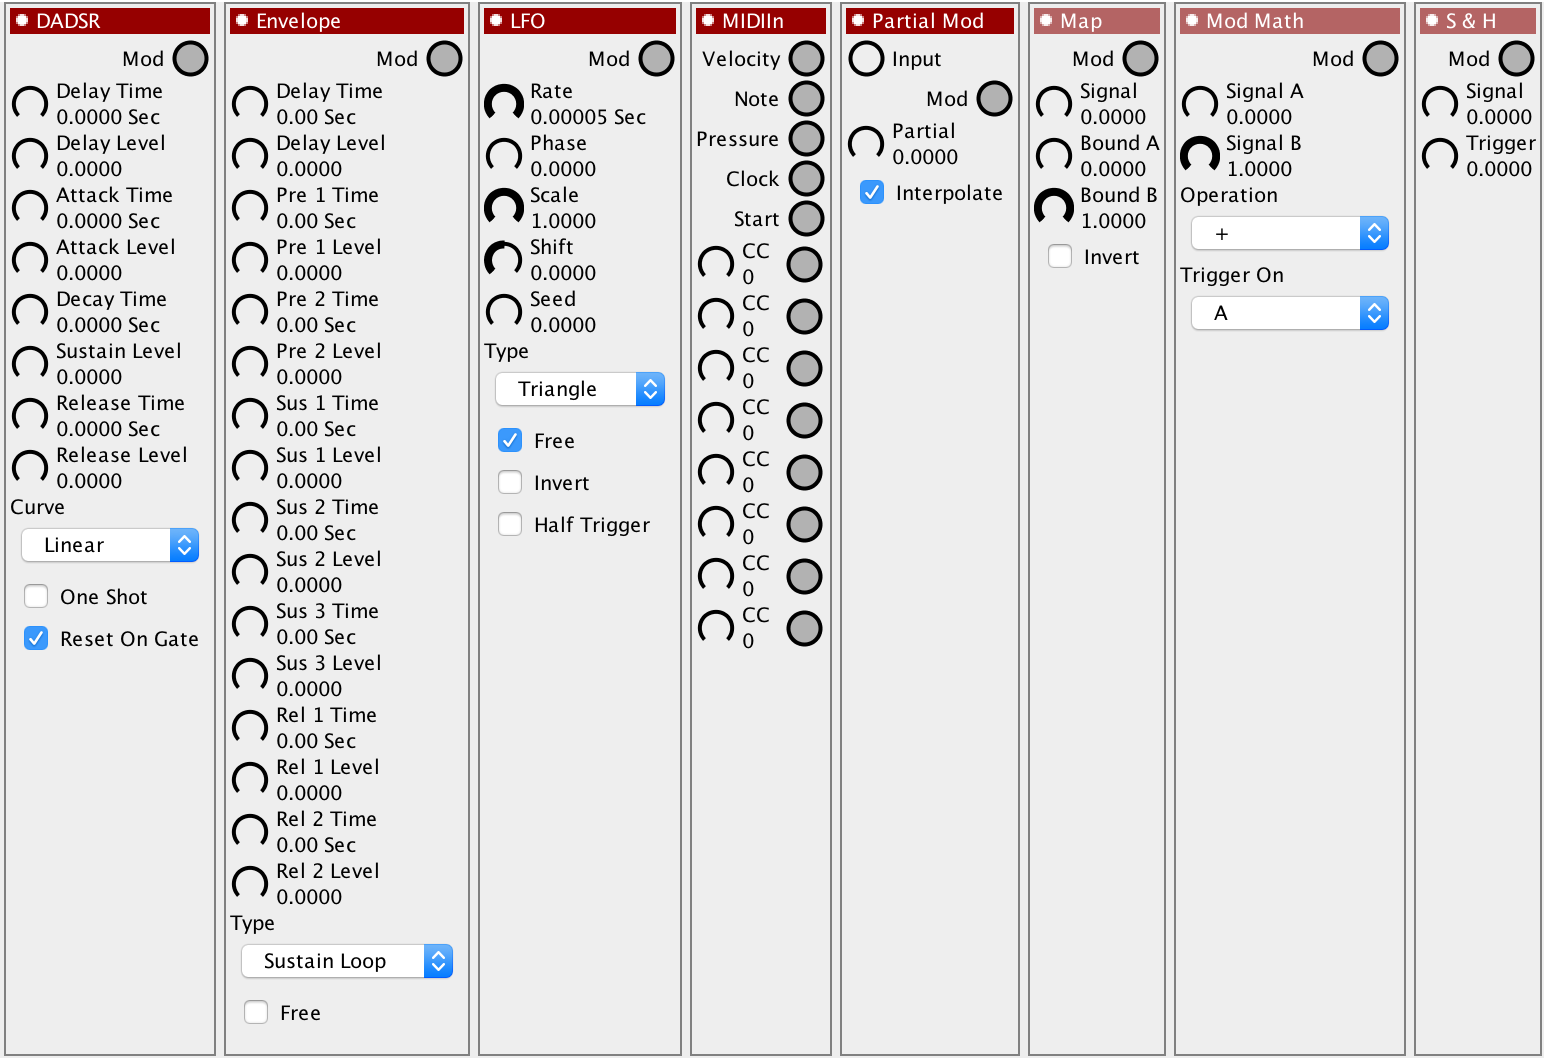
\includegraphics[width=6in]{ModulationSourcesAndShapers}\end{center}
%\caption{Modulation Sources and Shapers}
%\end{figure}



\subsection{Modulation Shapers}

\paragraph{Either/Or}  A switch which chooses among up to four outputs.  You choose the number of outputs with {\it Options}.  Thereafter, whichever output is currently being referenced by the value in {\it Input} will receive the value of {\it Yes}.  All other outputs will receive the value of {\it No}.  Either/Or is particularly useful with {\bf Mix}, where it can be used to zero out the amplitudes of all the mix inputs except for one, allowing you to choose from among several inputs.  See also {\bf Mix}.

\paragraph{Geiger}  A source of randomness in timing.  When it receives an input {\it Trigger}, Geiger outputs a trigger (and switches from modulation of 0.0 to 1.0 or vice versa) only with a certain random probability.  If {\it Trials} is 1, then the probability is simple: it's just the probability specified by the {\it Prob} dial.  If {\it Trials} is \(>1\), then every time Geiger decides to output a trigger (with the given probability), it instead increments a counter.  When that counter is  \(\geq\){\it Trials}, only then does Geiger output a trigger, and the counter is reset to 0.  The effect of this is that as {\it Trials} is increased, the effective variance between fast and slow intervals is reduced: but you'll also need to increase the rate at which you provide incoming triggers to keep things at about the same speed.\footnote{In case you were interested, Geiger's random number events are using a {\it Negative Binomial Distribution}.  Following https:/\!/en.wikipedia.org/wiki/Negative\_binomial\_distribution\ \ Geiger's Trials dial specifies the {\it r} parameter, and the Prob dial specifies \(1-p\).  When Trials is 1, then this simply the {\it Geometric Distribution}, and following https:/\!/en.wikipedia.org/wiki/Geometric\_distribution the Prob dial specifies the value {\it p}.}  Geiger also has a {\it Seed} for its randomness.  If the Seed is 0, then Geiger uses a nondeterministic random source: otherwise the random sequence is always the same every time a note is played, and that sequence is specified by the Seed.

\paragraph{Map}  Takes an incoming modulation signal and two values, \(A\) and \(B\).  If {\it Inverse} is not checked, the signal is then stretched such that what used to be 0.0 is now \(A\), and what used to be 1.0 is now B.  That is, if the incoming value is \(x\), then the outgoing value \(y = A + (B - A)x\).  If {\it Inverse} is checked, it's the opposite mapping: what used to be \(A\) (or lower) is now 0.0, and what used to be \(B\) (or higher) is now 1.0.  The point of {\it Inverse} is that you can use a Map to map a modulation value, then use another Map to {\it unmap} that modulation value back to its original range.  You also have the option of {\it Flip}ping \(x\) first, that is, setting it to \(1-x\) (if {\it Inverse} is checked, Flipping happens at the end).  Map has a final option called {\it Center}.  If this is checked, then instead of directly specifying \(A\) and \(B\) as bound for your range, you instead specify a {\it Center} and a {\it Variance} of the range, which is often more convenient.  The bounds are thus defined as \(A = \min(0,\ \text{\it Center} - \text{\it Variance})\) and \(B = \max(1,\ \text{\it Center} + \text{\it Variance})\).

\paragraph{Mod Math}  This module performs a variety of operations on incoming modulation signals \(A\) and \(B\), outputting the result.  It also can do some logic on the incoming trigger.  Operations:

\begin{itemize}
\item \(\boldsymbol{+}\)\quad Does \(\min(A + B,\ 1)\)
\item \(\boldsymbol -\)\quad Does \(\max(A - B,\ 0)\).  By setting \(A=0\), you can also use this to negate \(B\).
\item \(\boldsymbol \times\)\quad Does \(A \times B\)
\item {\bf min}\quad Does \(\min(A, B)\)
\item {\bf max}\quad Does \(\max(A, B)\)
\item {\bf square}\quad Does \(\min(A^2 + B,\ 1)\)
\item {\bf sqrt}\quad Does \(\min(\sqrt{A} + B,\ 1)\)
\item {\bf cube}\quad Does \(\min(A^3 + B,\ 1)\)
\item {\bf discretize}\quad Discretizes \(A\), using \(B\) to set the amount of discretization (from 1 to 128 chunks).
\item {\bf map hi}\quad Does \(A \times (1-B) + B\).  This ``inverts'' A under B.
\item {\bf average}\quad Does \((A + B) / 2\)
\item {\bf threshold}\quad If \(A \geq B\), returns 1, else returns 0.
\item {\bf switch}\quad If \(B\) more recently triggered than \(A\), then \(B\), else \(A\)
\end{itemize}

\noindent Additionally, there are a number of operators on triggers.

\begin{itemize}
\item {\bf A}\quad Triggers on A's trigger only.
\item {\bf A or B}\quad Triggers on A's trigger or on B's trigger.
\item {\bf A and B}\quad Triggers only when A's trigger and B's trigger coincide.
\item {\bf A and not B}\quad Triggers only when A's trigger occurs but B's trigger does not.
\item {\bf 2 A} {\it through} {\bf 192 A}\quad A rate divider.  Triggers every \(N\) triggers of A.  This is particularly useful in conjunction with {\it MIDI Clock} information from the {\bf MIDI In} module.\footnote{Note that if you're dividing a MIDI Clock pulse, some of these divisions might be useful for specifying note lengths:\\
\\
\begin{tabular}{rlrlrl}
	1&	Eighth Triplet (Triplet 64th Note)	&12&	Eighth Note							&48&	Half Note		\\
	2&	Quarter Triplet (Triplet 32nd Note)	&16&	Quarter Note Triplet					&64&	Whole NoteTriplet\\
	3&	Thirty-Second Note				&18&	Dotted Eighth Note				&72&	Dotted Half Note\\
	4&	Half Triplet (Triplet 16th Note)		&24&	Quarter Note				&96&	Whole Note\\
	6&	Sixteenth Note					&32&	Half Note Triplet				&144&	Dotted Whole Note\\
	8&	Triplet								&36&	Dotted Quarter Note									&192&	Double Whole Note\\
\end{tabular}\vspace{1em}
}
\item{\bf dir}\quad Triggers when A's value changes direction.
\item{\bf center}\quad Triggers when A's value crosses the center line (0.5).
\end{itemize}

\paragraph{S \& H}  Sample and Hold.  Takes an incoming modulation signal and a trigger.  If the type is {\it S \& H}, then on receiving the trigger, it samples the signal and outputs that value until the next trigger, when it resamples, etc.  If the type is {\it T \& H} or {\it T \& H 2}, then we are in {\it Track and Hold} mode.  Here, the trigger {\it toggles} between sampling and holding the value, or letting it pass through normally.  The difference between the two Track and Hold modes is just one of phase: in the first version, when a gate is received, we are in sample-and-hold mode, where as in the second version, when a gate is received, we are in pass-through mode.

\paragraph{Seq}  A step sequencer of up to 32 steps, as specified by {\it Steps}.  Each step is a modulation value which you can set.  On note-on, the sequencer resets itself to step 1, and begins incrementing each time the {\it Trigger} is fired.   If {\it Stop on Release} then on note-off the sequencer stops, otherwise note-off is ignored.  If {\it Free} is true, then the sequencer is free-running and ignores both note-on and note-off.    

The value of the current step is outputted as {\it Mod}.  When {\it Sample} is true, then {\it Mod} outputs the value of the current step as sampled immediately upon transitioning to that step; but if {\it Sample} is false, then the value of the current step may be changed in real-time, and {\it Mod} will output whatever its current value is.  {\it Mod} also outputs a trigger each time the step is incremented: you can use this to reset a sound to its start. 

Seq doesn't just read trigger values from {\it Trigger}: it also reads modulation values.  This can be used in two ways.  First, you can use the modulation value to slide the sequencer from one step value to another.  Specifically, {\it Change} specifies how the sequencer interpolates from one step to the next: the default is {\it Step}.  Interpolation is based on the incoming modulation value: if you're using an LFO, try setting it to Sawtooth.  You can get the opposite interpolation waves by setting the LFO to an inverted Sawtooth.   Second, if {\it Guided} is true, then the {\it Trigger} not only specifies when a step occurs, but its modulation value also specifies {\it which} step is performed, rather than incrementing the step as normal.

In addition to sequencing modulation signals, Seq can also be used in combination with {\bf Shift} to sequence note values.  To do this, attach {\it Mod} to Shift's {\it Shift} port, and set Shift's {\it Bound} to 1/3 and its {\it Type} to {\it Pitch}.  Feed the sound into Shift's {\it Input}, and the result in Shift's {\it Out}.  In this arrangement, each of Seq's modulation dials ranges from two octaves below to two octaves above.  To make things easier, if you double-click on a modulation dial, you'll get a pop-up menu with a keyboard, from two octaves below to two octaves above.  ``Middle C'' is 0.5 (the keyboard is keyed in C, but it'll be relative to whatever the current pitch is).  See also {\bf Shift}.

\paragraph{Soften}  A modulation signal smoother.\footnote{So why isn't this called Smooth?  Because there's another module called Smooth: see later in Section~\ref{unitshapers}}  Takes an incoming modulation signal and a degree with which to smooth it.  You can also specify whether or not Soften is free-running or always resets on gate.   Because softening will often significantly reduce the amplitude of a signal, Soften has an additional modulation, {\it Scale}, which lets you scale it back up.


\paragraph{User}  A tool for user control over modulation signals, mostly for testing.  User contains four modulation inputs, each of which is simply directly connected to a modulation output.  Thus if you connect the modulation output to multiple items, you can change all of them by changing the single input knob. Additionally there are four trigger buttons: pressing a button will issue a trigger to the associated modulation output.

%\begin{figure}[t]
%\begin{center}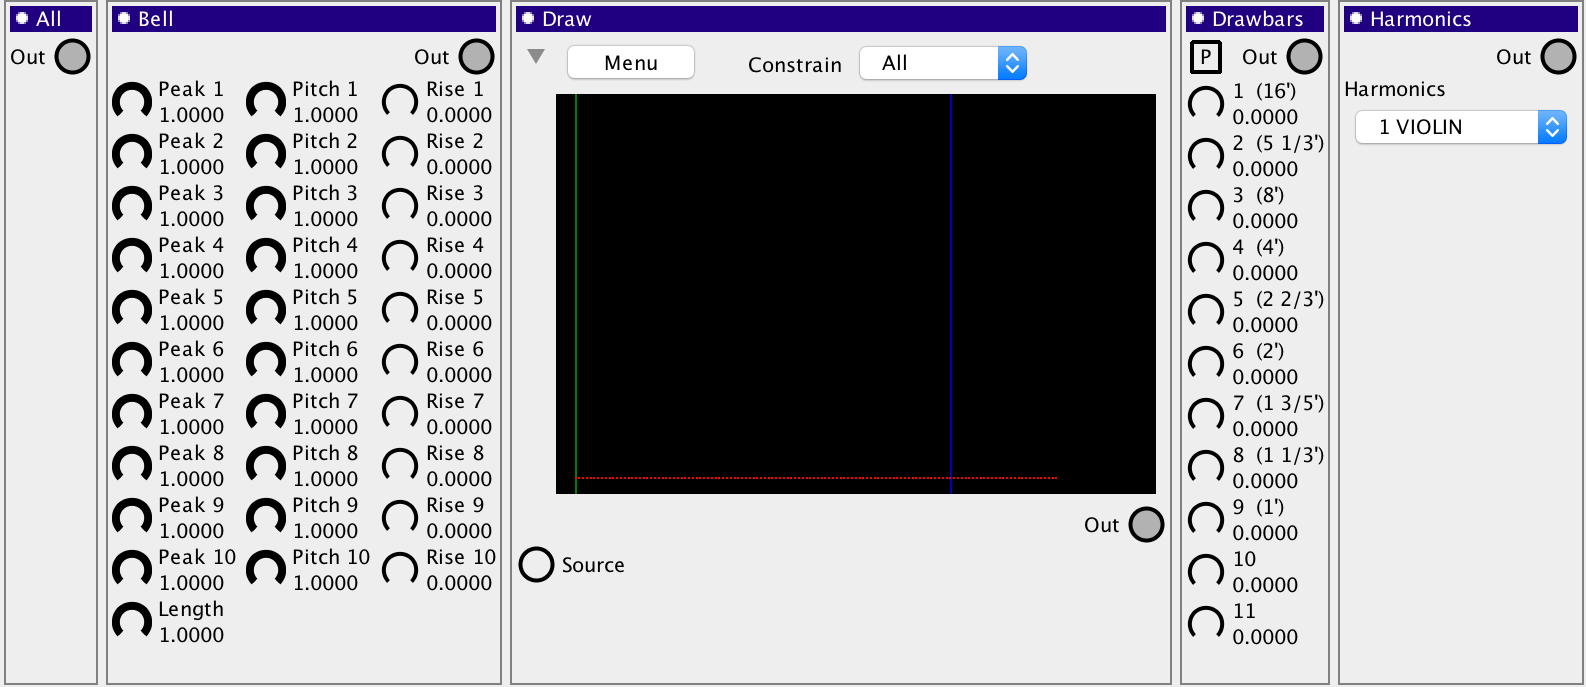
\includegraphics[width=6in]{UnitSources1}\end{center}
%\caption{Partials Sources (1)}
%\end{figure}


\subsection{Partials Sources}

\paragraph{All}  Outputs all partials, standardized, at full amplitude.  Useful for later shaping.

% --- Bell is not completed yet -- 
%\paragraph{Bell}   An experimental bell module (not working yet) which lets you specify the pitch, peak amplitude, and attack/decay of 10 different bell partials, in addition to the total length.

\paragraph{Draw}   Lets you draw partials, which are then output,   You can constrain the partials being drawn to a variety of subsets.  When you click on the {\it Menu} button, you can also save your scribbles and load them again, clear them, maximize, normalize, and standardize them, and (importantly) take a snapshot of partials from an incoming source.  The module can be collapsed to a smaller size if you wish.

Draw also allows you to load {\it single-cycle waveforms}, that is, sound files which start and end at zero and represent a single cycle of a sound wave.  You can do this by choosing {\it Load Wave...} from the {\it Menu} button.  These must be WAV files, mono, and cannot be very long (presently at most 2048 samples).  After loading, Flow converts them (naturally) into harmonics.

A good source of single-cycle waves is the AdventureKid Single Cycle Waveforms collection, available at https:/\!/www.adventurekid.se/akrt/waveforms/\quad Flow can read all of these.

See also {\bf Waves}, which contains harmonics of single-cycle waves from certain well-known synthesizers.

\paragraph{Drawbars}   Produces the sine wave equivalents of the drawbars of a classic tone wheel organ.  There are a number of preset options.

\paragraph{Harmonics}  Outputs the first 16 harmonics, whose amplitude you can define independently.  You optionally can load these harmonics from a source. See also {\bf Partials}.

\paragraph{KHarmonics}  Produces a wide range of partials drawn from patches from the Kawai K5 synthesizer, including both factory patches (with Kawai's permission) and various patches in the public domain.  You have the additional option of {\it Normalizing} the partials.  Note that among the harmonics are ones purporting to be drawn from the Kawai K3.  These are just wrong.  However the {\bf Waves} module has the correct ones.

See also {\bf Waves}, a similar collection drawn from various other synthesizers.


%\begin{figure}[t]
%\begin{center}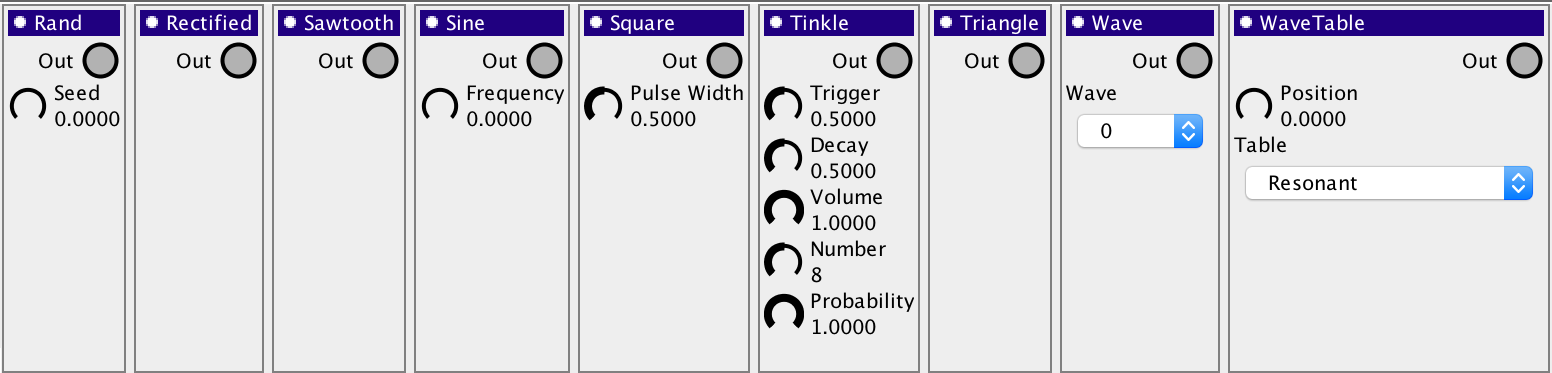
\includegraphics[width=5.8in]{UnitSources2}\end{center}
%\caption{Partials Sources (2)}
%\end{figure}

\paragraph{Noise}  Random noise, hiss, etc.  This is done by creating and immediately destroying entirely random partials independent of the pitch.  You can specify the number of partials being used (you can get away with surprisingly few to make a good hiss).   To change the color of the partials: you can also specify the high and low frequency bounds for the partials; you can create a ramp in amplitude from the low to high partials; and you can specify the degree of variance in amplitude among the random partials.  Finally, you can set the average volume (the gain) of the hiss.  This module is designed to merge with other sources to add hiss to them: most commonly, you would use it as the primary source in the {\bf Fill} module.  To make this convenient, by default the partials used are the highest numbered ones: the lower ones are all set to amplitude 0 and frequency 0.0.  However if you use this in combination with a merging option like {\bf Combine} which steals from the high partials, or other adjusters like {\bf Fatten}, you'd want the low partials to be used.  By setting {\it Top} to false, you can cause the low partials to be used for the hiss, with the remainder set to amplitude 0 and a frequency somewhat beyond the high frequency bound.

\paragraph{Partials}  Outputs 16 partials whose amplitude and frequency you can define independently.  You optionally can load these partials from a source.  See also {\bf Harmonics}.

\paragraph{PartialLab}  Allows you to describe a sound as a combination of three mathematical functions operating on your harmonics.  For each of the three, you can define the function type, a function parameter, the gain of the function, and the harmonics the function manipulates.  When multiple functions manipulate the same harmonic, the earlier function takes precedence.  {\bf Important Note 1}\quad Unlike standard constraints menus, PartialLab's constraints menus include ``All'' at the end.  {\bf Important Note 2}\quad This is a costly module if you are modulating any of these values in real time, perhaps by an LFO (there are many calls to \(x^y\)): you can do it, but it'll keep your laptop warm.

\paragraph{Rand}  Random partials.  Outputs all partials, standardized, with random amplitudes.  If the seed is 0, then the amplitudes are different each gate; otherwise they are the same random values each gate, using a random number generator with the given seed.

\paragraph{Rectified}  The harmonics of a rectified sine wave, that is, \(|\sin(x)|\).

\paragraph{Sawtooth}  The harmonics of a sawtooth wave.

\paragraph{Sine}  A single harmonic at 1.0 amplitude.  The harmonic can be any partial frequency from 1.0 to 128.0.

\paragraph{Tinkle}  Produces random partials, creating a tinkling effect.  Some {\it number} of new partials are created whenever the {\it trigger} occurs, and at the given {\it volume}.  The partials {\it decay} at some rate.  The {\it probability} specifies the likelihood that partials will be created when a trigger occurs.

\paragraph{Triangle}  A triangle wave.  Note that normally triangle waves include negative amplitude harmonics, that is ones with inverted phases.  As {\name} does not produce phases, these harmonics become all positive (you likely won't hear a difference).

\paragraph{Waves}  A collection of harmonics drawn from single-cycle waves in the Kawai K3, Ensoniq SQ-80, and Sequential Prophet VS.  These are as best as I can do for now\,---\,they may change if my sources improve.  The Kawai K3 harmonics are complete: obviously wave 31 is missing since that's actually the user's additive harmonics space.\footnote{The K3 harmonics are from http:/\!/www.deepsonic.ch/deep/audio\_samples/kawai\_k3\_-\_samples\_-\_33\_waveforms.mp3 by deep!sonic (http:/\!/www.deepsonic.ch)}

The SQ-80 is unusual in that it had different oversampled versions of the same wave depending on the octave of the note played on the keyboard.  The harmonics here are taken from the lowest octaves (with the most harmonics).  This collection is incomplete: the original source had some errors.\footnote{The SQ-80 harmonics are drawn from the waves in http:/\!/www.buchty.net/ensoniq/files/the\_waves.zip by //christian.}

The Prophet VS traditionally had waves 32--127, and these more or less line up with the harmonics provided by Flow: but you'll notice that Flow is missing a few because the original source is missing them.  Some, but not all, of the missing waves don't matter.\footnote{The Prophet VS harmonics are drawn from https:/\!/www.dropbox.com/sh/ja0tc8wn6cnudzj/AACYqe2mjrWU2CeXIttm6MhOa as discussed in the forum thread http:/\!/www.muffwiggler.com/forum/viewtopic.php?t=33918\&sid=9e0b9554f0ac483b62a88c074c6136c3}

See also {\bf Draw}, which allows you to load single-cycle waves: the manual section on Draw has good suggestions for sources of these waves.

See also {\bf KHarmonics}, a similar collection drawn from various Kawai K5 harmonics.

\paragraph{Wavetable}  Lets you load wavetables (as ``.WAV'' files) from https:/\!/waveeditonline.com/, then wander through them using the provided modulation.  You can turn off interpolation between waves.

You can also load an arbitrary sound directly and Flow will chop it up into a wavetable for you.  Your sound file must be a 16-bit signed integer WAV file, mono only.  You should turn on the {\it sampled} option prior to loading the sound, which will cause Flow to grab larger overlapping chunks and to use a windowed FFT (the {\it sampled} option doesn't do anything but affect how the sound is loaded).  The sampled option is designed to remove some of the choppiness from reading an arbitrary sound, but it won't remove all of it.  You can eliminate most of the rest by running the partials through a Smooth module set to about 0.5.  Note: this is only for sampling arbitrary sounds:  you don't want to do any of this stuff (the sample option, Smooth) if you're reading a prepared wavetable from https:/\!/waveeditonline.com/.


\subsection{Partials Shapers}
\label{unitshapers}


All of the shapers have the ability of being {\bf constrained}.  This means that you can tell the shaper to {\it only} perform its operation on certain partials; the others should be left as they are.\footnote{If a shaper has multiple partials sources, then ``left as they are'' means that they should be reverted to whatever values they had in the first partials source.  For example, in Amp Math the first partials source is A.}  The constraint facility (Figure~\ref{constraintfacility}) is at the bottom of the shapers and consists of three widgets.  First, there is a pop-up menu (combobox) where you can specify common constraints.  Above it is a checkbox labelled {\bf Not}, where you can optionally flip things: that is, specify that you want to perform the operation on everything {\it but} the partials in question.  Finally, there is a {\it constraint partials source}, labelled {\bf Only}. If you attach a unit's output to this, then its incoming partials indicate what the constraint should be: specifically, the partials that will be constrained will be those whose positions match up with non-zero amplitude partials coming into the constraint partials source. For example if the constraint partials source has non-zero amplitudes for partials 4, 7, and 9, then this tells the shaper to constrain its outputted partials 4, 7, and 9.  The constraint partials source overrides the pop-up menu.

Okay, here we go.

%\begin{figure}[t]
%\begin{center}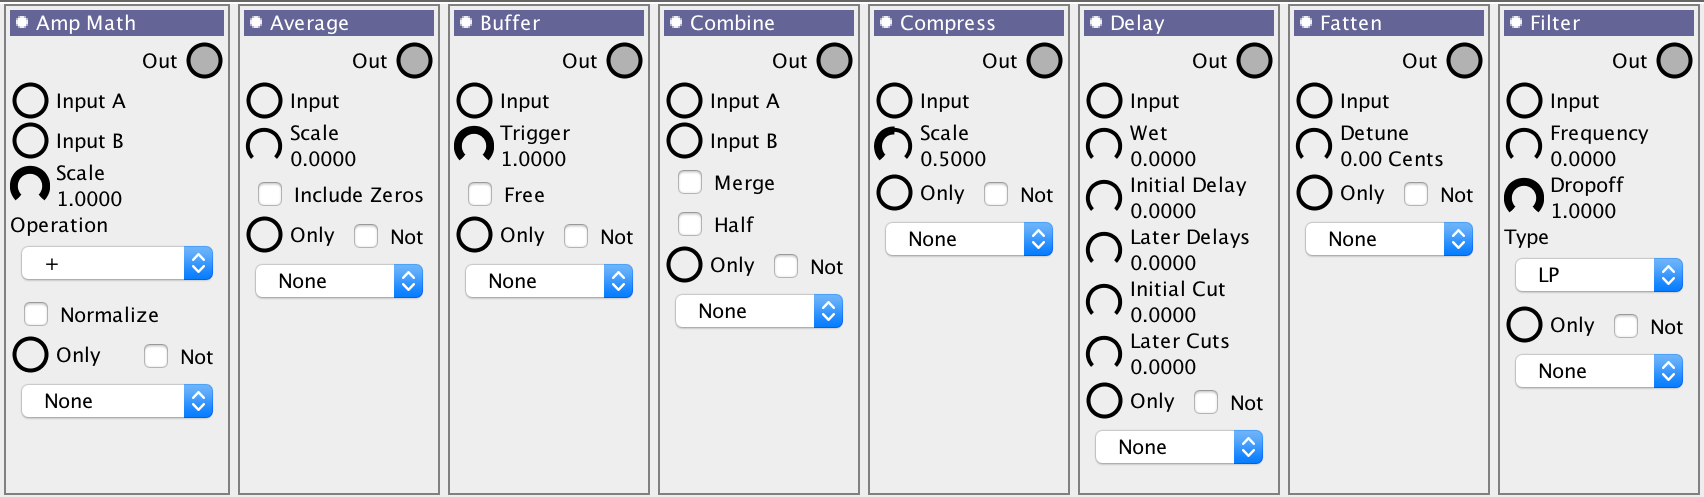
\includegraphics[width=6.5in]{UnitShapers1}\end{center}
%\caption{Partials Shapers (1)}
%\end{figure}


\enlargethispage{1em}

\paragraph{Amp Math}  This shaper modifies the partials from two sources \(A\) and \(B\) by putting every pair of them \(\langle A_i, B_i\rangle\) through the same function, along with a modulation source \(M\).  The operations are:

\begin{itemize}
\item \(\boldsymbol{+}\)\quad Does \(A_i + B_i + M\)
\item \(\boldsymbol -\)\quad Does \(\max(A_i - B_i - M,\ 0)\)
\item \(\boldsymbol \times\)\quad Does \(A_i \times B_i\)
\item {\bf inv} \(\boldsymbol \times\)\quad Does \(A_i \times (1 - B_i)\)
\item {\bf compress}\quad Does \(1 - (1 - A_i) \times (1 - B_i)\)
\item {\bf average}\quad Does \(M \times A_i + (1 - M) \times B_i\)
\item {\bf min}\quad Does \(\min(A_i \times (1 - M), B_i)\)
\item {\bf max}\quad Does \(\max(A_i \times (1 - M), B_i)\)
\item {\bf filter}\quad If \(B_i < M\) then returns 0, else \(A_i\)
\item {\bf filter not}\quad  If \(B_i \geq M\) then returns 0, else \(A_i\)
\item {\bf fill}\quad If \(A_i > M\) then returns \(A_i\), else \(B_i\)
\item {\bf threshold}\quad If \(A_i > M\) then returns 1 else 0
\item {\bf scaledown}\quad Does \(A_i \times M + B_i\)
\item {\bf scaleup}\quad Does \(A_i \times (M + 1) + B_i\)
\item {\bf scalefar}\footnote{Scales in a range 1...10 rather than 1...2 for {\it scaleup}}\quad Does \(A_i \times (M + 9) + B_i\)
\item {\bf clampdown}\quad Does \(\min(A_i, M) + B_i\)
\item {\bf clampup}\quad Does \(\max(A_i, M) + B_i\)
%\item {\bf remove}\quad If \(i\ \text{mod} (M \times 127) = 0\) then returns \(A_i\), else \(B_i\)
\end{itemize}

You have the option of normalizing the resulting partials.   Be sure to read ``Mixing Strategies'', Section~\ref{mixingstrategies}.  See also {\bf Combine} and {\bf Fill} and {\bf Mix} and {\bf Morph}.

\paragraph{Average}  Computes the average amplitude of all the partials, then nudges the amplitudes of all the partials towards the average.  The amount of nudging is an incoming modulation.  You can specify whether to include the zero-amplitude partials in the average.

\paragraph{Buffer}  This is a sort of Sample and Hold for partials.  Every time Buffer receives an incoming trigger, it takes a snapshot of its input and uses that snapshot for its output.  Buffer can be constrained, which means that it outputs its snapshot for certain partials, while outputting the current source partials for the remainder.

\paragraph{Combine} The partials from two sources are merged by throwing together all the partials from both sources.  Then we take the lowest frequency partials, over both sources, then the next lowest frequency partials, and so on, until we have enough partials.  The remaining (higher frequency) partials are discarded.  You can scale (down) the amplitude of each of the incoming sources.  Combine has two options.  First, you can indicate that partials of identical frequency aren't added separately but are rather merged together (their amplitudes are added), which allows us to include more partials but tends to create unusual discontinuities if the sources are changing in frequency relative to one another.  Second, you can indicate that exactly half of the chosen partials must come from each source.  This is useful if the two sources differ greatly in frequency, so one will dominate the combination.  Be sure to read ``Mixing Strategies'', Section~\ref{mixingstrategies}, particularly if you're hearing pops.  See also {\bf Amp Math} and {\bf Fill} and {\bf Mix} and {\bf Morph}.

\paragraph{Compress}  The amplitude of every partial is raised to a certain power, controlled by the {\it Scale} modulation.  If Scale is greater than 0.5 (the mid-point), then the amplitude is raised and compressed more and more, resulting in them getting louder and with less difference among them.  If Scale is less than 0.5, then the opposite happens: the amplitudes are {\it expanded}, resulting in a larger difference among them, and with them all getting quieter.

\paragraph{Delay}  Partials are added to an initial one-shot delay, then a repeated delay.  Each delay has a length (the ``delay'') and a cut (how much to cut down the delayed sound).  You can also specify the wet/dry ratio.

\paragraph{Dilate} If a partial has a neighbor partial which is {\it larger} than it, then its amplitude is increased towards its neighbor: this change trickles down to its further (smaller) neighbors as well.  This has the effect of boosting neighboring partials until ultimately all partials are the same amplitude.  {\it Boost} is the amount to increase.  You can specify whether only left neighbors, right neighbors, or both are considered.  See also {\bf Skeletonize} (which is almost, but not quite, the opposite concept).

\paragraph{Fatten}  The top half partials are discarded and reused to create detuned versions of the lower half partials.  The detuning amount is specified as well as the wet/dry ratio.

\paragraph{Fill}  Given two incoming sources \(A\) and \(B\), this module first adds all of the non-zero-partials of \(A\) to the output; any remaining partials are filled from non-zero amplitude partials in \(B\), starting at its lowest frequency partials and working up.  You can scale (down) the amplitude of each of the incoming sources.  This module is particularly useful with {\bf Noise}.  Be sure to read ``Mixing Strategies'', Section~\ref{mixingstrategies}.  See also {\bf Amp Math} and {\bf Combine} and {\bf Mix} and {\bf Morph}.

\paragraph{Filter}  This is a resonant state-variable 2- or 4-pole filter. You can sweep through High Pass (at 0.0) to Notch (at 0.25) to Low Pass (the default, at 0.5), to Band Pass (at 0.75) and finally to High Pass again (at~1.0).  Resonance values currently range from no resonance (that is, resonance \(Q=\frac{1}{\sqrt{2}}\)) at 0.0 to ten times that amount (\(Q =\frac{10}{\sqrt{2}}\))  at 1.0.  And you can, of course, set the cutoff frequency.

Filter can be set to be {\it Relative}.  This means that the filter cutoff frequency is set to be relative to Middle C.  If you're playing a higher note, the cutoff frequency will automatically be set higher to match; similarly if you're playing a lower note, the cutoff frequency will be automatically lower.

%\begin{figure}[t]
%\begin{center}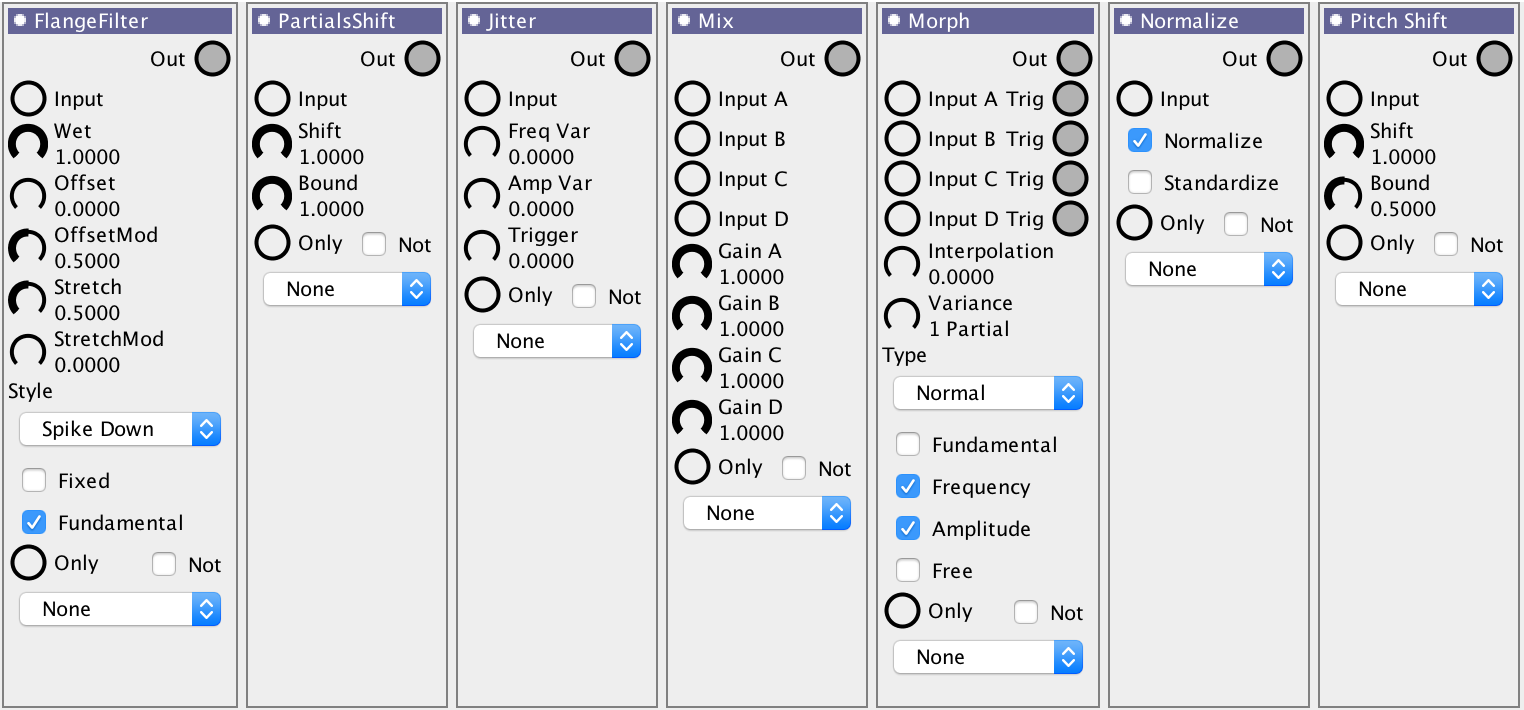
\includegraphics[width=6in]{UnitShapers2}\end{center}
%\caption{Partials Shapers (2)}
%\end{figure}


\paragraph{Flange Filter} This filter simulates various flanging, phasing, and chorusing effects via rough approximations of comb filters.  You can select what kind of comb filter shape you'd like (``spike down'' is the classic for flanging and chorusing etc.).    You can also stipulate whether the filter shifts to follow the pitch of your note or is fixed in the frequency location of its lobes.    The flange filter has several confusing dials.  {\it OffsetMod} is similar, lets you modulate the lobe positions.  {\it Stretch} lets you specify the size of the lobes.  {\it StrechMod} is similar but meant to have a modulation source attach to it.  You can also specify the wet/dry ratio. {\bf Hint:}  the {\it degree} of OffsetMod or StretchMod is very high, but you can reduce this by changing your LFO's Scale value.  The LFO's shift is also interesting to play with.

\paragraph{Rotate}  This takes all the partials within some frequency range from \(A\) to \(B\) certain range and shifts all their frequencies by some value \(X\) (where \(A \leq X \leq B\).  Partials shifted to beyond \(B\) are wrapped around to be back in-range, so this has the effect of rotating all the partials.  Rotation is usually modulated using an LFO set to a sawtooth or inverse sawtooth.

There are a number of options.  First, you can {\it stretch} the partials to a non-linear scaling, such as \(x^2\) or \(x^8\).  Second, you can {\it window} the amplitudes so that the partials at either end are scaled down in volume.  This windowing can have its center either in the middle of the range (if {\it center} is true) or can be stretched to match the stretched partials.  You have the option of {\it soloing} the rotation: muting all the partials other than those involved in rotation.  Finally, you can {\it thin} out some number of partials; this often creates a better sounding tone for rotation.
 
\paragraph{Shift} This shifts all the partials in your input in a certain way.  {\it Shift} specifies by how much (this is easily modulated), and {\it Bound} scales the shifting.  There are three ways you can shift.  First you can shift the {\it Pitch}: this is essentially multiplying the partials by a certain amount.  Second, you can shift the {\it Frequency}: this {\it adds} a certain amount to the partials, which creates an inharmonic shift effect.  Third, you can shift the {\it Partials}: this shifts the whole partial amplitude array up or down.  A warning about partials shifting: this can make abrupt changes in amplitude, and you may hear static-like clicks or pops, especially in low pitches.  You can clean this up by running things through {\bf Smooth} set to about 0.9. See also {\bf Seq}.  Finally, {\it Vibrato} is the same as {\it Pitch}, but with a much smaller bound: at maximum, the bound is one whole step (major second) in each direction.  This makes it easier to dial in precise vibrato amounts.

\paragraph{Linear Filter} This is a filter where you can specify up to 8 nodes (points of change) in terms of frequency and gain.  The filter then just draws lines attaching the nodes, and this becomes the filter frequency function.  Nodes are always sorted first by frequency.  {\it Num Nodes} is the number of nodes being used.

Linear Filter can be set to be {\it Relative}.  This means that the filter cutoff frequency is set to be relative to Middle C.  If you're playing a higher note, the cutoff frequency will automatically be set higher to match; similarly if you're playing a lower note, the cutoff frequency will be automatically lower.  See also {\bf Partial Filter}.

\paragraph{Jitter} You can add jitter to either the frequencies or the amplitudes (or both) of your partials.  The amount of noise is controlled by {\it Freq Var} and {\it Amp Var} respectively.  The {\it Trigger} informs the module to add noise to its current jitter configuration.  You can also specify that Jitter should {\it only} apply to non-zero partials this is useful when using Jitter along with Fill.

\paragraph{Mix} This is a straightforward mixer: the amplitudes of the partials of four different inputs can be mixed, with their respective gains.  The {\it frequencies} of the partials are set to those of the first input whose amplitudes are non-zero.  In many cases, it's likely that all four inputs have partials with the same frequency, so it wouldn't matter.  But this strategy is also useful because it allows Mix to be used in combination with {\bf Either/Or} to select a single output among the four mix inputs.  Be sure to also read ``Mixing Strategies'', Section~\ref{mixingstrategies}.  See also {\bf Either/Or} and {\bf Amp Math} and {\bf Combine} and {\bf Fill} and {\bf Morph.}

\paragraph{Morph} This module morphs (interpolates) between two or more inputs.  In the most basic configuration, when two signals are morphed together, the amplitudes of their partials are weighted and averaged, and the frequencies of their partials are {\it also} weighted and averaged.  The weighting constant \(\alpha\) is controlled by the {\it Interpolation} knob.  For example, consider Inputs X and Y.  For each pair of partials \(\langle P^X_i, P^Y_i\rangle\) in X and Y respectively, with frequencies \(\langle F^X_i, F^Y_i\rangle\) and amplitudes \(\langle A^X_i, A^Y_i\rangle\), we produce a final partial \(P_i\) whose frequency \(F_i = (1-\alpha) F^X_i + \alpha F^Y_i\) and whose amplitude \(A_i = (1-\alpha) A^X_i + \alpha A^Y_i\).

You have the option of turning on or off morphing of the frequency or amplitude.  You can also tell Morph to {\it not} morph the fundamental.  

That's the simple case.  But there are several other bells and whistles in Morph.  First, you can have more than two inputs.  In this case, when Input A has finished morphing into Input B, Morph will then switch to morphing Input B into Input C, then C into D, and then D into A, looping back around again.  Morph decides to switch when the direction of the interpolation signal changes.  For example, suppose you had a triangle LFO attached to the Interpolation.  A the LFO goes up, A is morphed into B.  Then as the LFO goes down, B is morphed into C.  As the LFO goes up again, C is morphed into D, and as it goes down again, D is morphed to A.  Some inputs change over time\,---\,when Morph switches to that input, we'd like a way to inform the input source to reset itself to prepare to be included in the Morph.  To do this, Morph sets the trigger for that Input (labelled {\it Trig}), which you can use as a preparation signal.

Second, normally every Partial \(i\) in the first Input is paired up with the same Partial \(i\) in the other input to morph to it.  But you can change what the pairing is with the {\it Type} popup.  These pairs include:

\begin{itemize}
\item {\bf Normal}\qquad Just the standard pairing.
\item {\bf Random}\qquad Partials are paired up at random with ``nearby'' partials.  The definition of how far away nearby could be is specified by the {\it Variance} knob.  The pairing is randomized every time a new note is played, or every time the {\it Variance} is modified.
\item {\bf 2-Pair, 4-Pair, 8-Pair}\qquad Partials are paired up in groups with other partials 2, 4, or 8 away from them.
\item {\bf Increasing}\qquad The first partials are paired.  Then the next two partials are paired in 2-pair fashion.  Then the next 4 partials are paired in 4-pair fashion, and so on.
%\item {\bf Rand \textit{N}}\qquad Random fixed presets of different variance, carefully chosen to be provide almost exact variance settings.  These sound random, but the pairings don't change every time you play a note, so you get the same effect each time (unlike {\bf Random}, where the effect changes every note).
\end{itemize}

%\begin{figure}[t]
%\begin{center}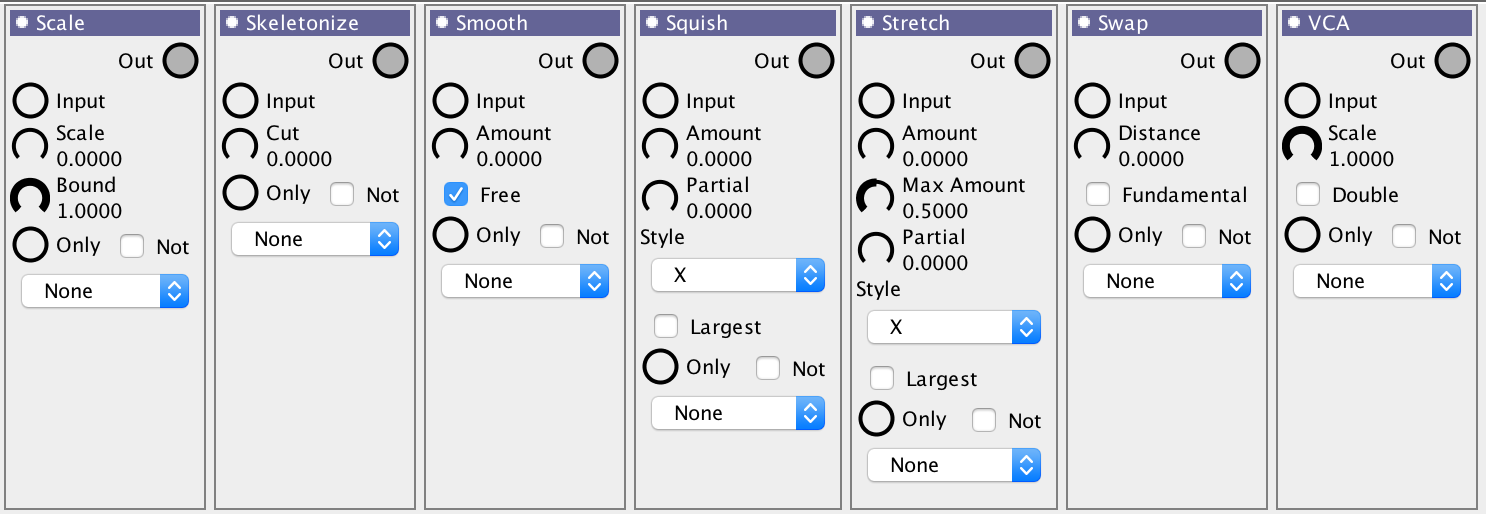
\includegraphics[width=5.7in]{UnitShapers3}\end{center}
%\caption{Partials Shapers (3)}
%\end{figure}


Finally, if {\it Free} is set, then Morph doesn't reset to Inputs A and B every time you press a note\,---\,it keeps morphing from wherever it left off.  Be sure to read ``Mixing Strategies'', Section~\ref{mixingstrategies}.  See also {\bf Amp Math} and  {\bf Combine} and {\bf Fill} and {\bf Mix}.

\paragraph{Normalize} This {\it normalizes} the input (scales it so that the amplitudes all sum to 1.0, creating a relatively consistent volume) or {\it maximizes} it (scaling it so that the highest amplitude equals 1.0).  Optionally it also {\it standardizes} it (sets all the frequencies to standard harmonic values).

\paragraph{Partial Filter} This is a filter based on the partials of an incoming signal.  The partials form nodes in the filter, and the filter function interpolates between them.  Try drawing partials with {\bf Draw} and feeding them into Partial Filter to filter some sound to get the idea.  

Partial Filter can be set to be {\it Relative}.  When relative, the partials are simply filtering their equivalent frequencies in the incoming sound.  When {\it not} relative, then the partial frequencies are fixed as follows.  A partial at position 1.0 (where the fundamental normally is), or indeed \(\leq 1.0\), would represent 0Hz, a partial at 2.0 would represent 100Hz, a partial at 3.0 would represent 200Hz, and so on.  Typical standardized partials (going from 1 to 128) would thus cover 0Hz to 12.7KHz.  That may not be far enough for you; but you can easily {\it double} this scale, so 1.0 is 0Hz, 2.0 is 200Hz, etc., clear up to 128.0 being 25.4KHz.\footnote{You could have stretched this with {\bf Scale} or {\bf Shift} too of course.}  See also {\bf Linear Filter}.

\paragraph{Pitch Shift} Pitch Shift scales the frequency of all the partials so that the sound is a higher pitch.  This is a multiplying effect, as opposed to PartialsShift, which is largely an additive effect.    {\it Shift} specifies by how much (this is easily modulated), and {\it Bound} scales the shifting.  See also {\bf Partials Shift} and  {\bf Scale}.

\paragraph{Scale} This scales the frequency of all the partials but keeps the pitch the same: it ``stretches'' the partials out away from frequency 1.0, or compacts them towards it.  A {\it Scale} value of 0.5 is no scaling: larger values stretch the partials, and smaller values compact them.   See also  {\bf Pitch Shift} and  {\bf Partials Shift}.

\paragraph{Skeletonize} If a partial has a neighbor partial which is {\it larger} than it, then its amplitude is cut by a percentage.  The percentage is a power of the distance of the partial to the peak partial on the left or right, whichever is further.  This has the effect of stripping partials out and only leaving the locally highest partials.  {\it Cut} is the base percentage.  See also {\bf Dilate}, which is almost, but not quite the opposite concept.

\paragraph{Smooth} This module smooths over the frequency and amplitude differences between successive sets of partials.  The degree of smoothing is specified by {\it Amount}.  Specifically, it maintains an internal set of Partials \(P\).  At every timestep, it takes the current incoming Partials \(Q\), and sets each amplitude \(A^P_i\) of \(P\) to \(A^P_i = (1-\alpha) A^P_i + \alpha A^Q_i\).  Likewise it sets each frequency \(F^P_i = (1-\alpha) F^P_i + \alpha F^Q_i\), where \(\alpha\) is the Amount.  Smooth has to deal with one unusual case: when the incoming partials of \(Q\) start wandering about in frequency and eventually cross one another.  This creates discontinuities in the smoothing.  Smooth handles this by trying to remember which partials were which; this strategy will work fine if Smooth is fed partials from the {\it first} partials output of any module.  No guarantees are made regarding other partials outputs.  Modules rarely have more than one output, anyway.

\paragraph{Squish} The frequencies of the partials are squished {\it towards} a specific target partial, which you can specify.  The degree of squishing is specified by {\it Amount}, and the squishing function can be \(x\), \(x^2\), or \(x^3\), where \(x\) is the distance between a partial and the target.  There are two versions of each squishing function: the ``free'' version, where all partials freely move towards the target, and the non-``free'' version, where partials are restricted to still range between the original minimum and maximum partials: think of the non-``free'' version as a spring whose center can move towards some partial, but whose ends are fixed to two walls: and the ``free'' version doesn't have ends fixed to anything.  See also  {\bf Stretch.}

\paragraph{Stretch} The frequencies of the partials are stretched {\it away} a specific target partial, which you can specify.  The degree of stretching is specified by {\it Amount}, scaled by {\it Max Amount}, and the stretching function can be \(x\), \(x^2\), or \(x^3\), where \(x\) is the distance between a partial and the target.  There are two versions of each stretching function: the ``free'' version, where all partials freely move away from the target, and the non-``free'' version, where partials are restricted to still range between the original minimum and maximum partials: think of the non-``free'' version as a spring whose rings can move away from some partial, but whose ends are fixed to two walls: and the ``free'' version doesn't have ends fixed to anything.  See also  {\bf Squish.}

\paragraph{Swap} This divides the partials into groups {\it Distance} in size, then reverses the partials in each group (swapping their frequencies).  You are given the option of not including the Fundamental among these groups.

\paragraph{Sub} Adds up to four partials at octave spacing below the fundamental, eliminating the top four partials.  You can specify the amplitude of the partials relative to the fundamental.

\paragraph{VCA} This is just what it says on the tin: an amplifier (VCA is the classic term).  A VCA is very commonly used in conjunction with an envelope.  It takes an input and multiplies all of its amplitudes by {\it mod} (which goes 0--1), then by {\it scale} (which goes 0--8).  The {\it mod} modulation is designed for you to attach LFOs or envelopes etc.  The {\it scale} modulation is not linear and so is just meant for you to dial in a maximum scale value.   The VCA also sports a {\it bass boost} meant to, well, boost lower partials.  It's very simplistic: at maximum boost, partials of frequency 0 are boosted \(2\times\), and partials at Nyquist are boosted \(0\times\).  Partials in-between are boosted in linear proportion to their position between these two extremes.  

\subsection{Special Modules}
\label{specialmodules}

There are currently five special modules: {\bf In}, {\bf Out}, {\bf Choice}, {\bf Fix}, {\bf Note}, and {\bf Macro}.  The {\bf Out} module is critical in every patch, and is discussed below in Section~\ref{outmodule}.  {\bf In} and {\bf Macro} enable {\it macros}\.---\,and {\bf Out} helps out here as well\,---\,as discussed below in Sectino~\ref{creatingmacros}.

\paragraph{Choice}  The Choice module is an odd duck: it doesn't produce any sounds or modulation at all.  Instead, it enables you to change a module's checkboxes and comboboxes using a modulation signal.  To do this, note that Choice has a modulation input and a sound input port both called {\bf Target}.   Plug one of your target module's modulation or sound outputs into the appropriate Target port: this tells Choice what target module it should be modifying.  Don't attach to both of them, or Choice will just use the sound input port.

After this is done, you will find you can select an option (a combobox or a checkbox) via the {\it Option} dial.\footnote{At present, the constraints facility is not part of the available options.  This might change in the future.} Once this is done, you can change the value of the selected option via the {\it Value} dial.  This might be particularly interesting to do via an LFO.

Note that when you change the value, it's not immediately reflected (or reflected at all!) in the target module's GUI.  This is because updating the GUI in real time could be very costly.  But it's been change!  You can convince yourself of this by dragging the module and moving it.  Similarly, if you click on the option combo box or check box, the result is not directly reflected in the Option dial.

\paragraph{Note} This module also doesn't process sound at all. Instead, it lets you leave a note or comment.  You can change the width of the Note panel with two arrow-like buttons at the bottom.   You can have as many Note modules as you like; they'll each save their comments independently as part of your patch.

\paragraph{Fix} This module likewise doesn't process any sound.  Instead, it lets you fix the note (pitch) being played, and/or the velocity being played, to specific values.  After Fix is called, it changes the pitch and volume, and all later modules will use the new ones: thus you want Fix early in your modules, ideally the very first one.  I use Fix in percussion patches to force the patches to always make the same pitched sound regardless of the note being played.

\subsubsection{The \textit{Out} Module in Basic Use}  
\label{outmodule}

Every useful patch has to have an Out module, since it provides the facility for outputting your final partials to the audio system.  Out does several important basic things:

\paragraph{Audio Generation}  Out is responsible for converting your partials into sound.  To do this, connect your final partials to the port on Out normally labelled {\bf A}: it's the topmost port in the module.  You can adjust the volume of this port by changing the {\it Gain} knob.

\paragraph{Reverb} Flow sports a simple implementation of the Freeverb algorithm.\footnote{A well regarded reverb algorithm in the public domain by ``Jezar at Dreampoint''.}  This algorithm has three parameters.  {\it Wet} is the dry/wet knob for the algorithm (0 is fully dry).  {\it Damp} is the damping: basically a low-pass filter applied to the reflected signals.  {\it Size} is the room size, which translates roughly into the reverb decay.  Note only a single sound (voice \#0) controls the modulation of Wet, Damp, and Size.  This means that if you attach an Envelope etc. to any of these modules, it may not respond in exactly the way you think.  It's probably best to keep them as knobs rather than attaching a modulation source.

\paragraph{Dephase} By default Flow keeps all of its partials consistent with their original phases, so when you output a Sawtooth it'll look like this:  \smash{\raisebox{-0.5em}{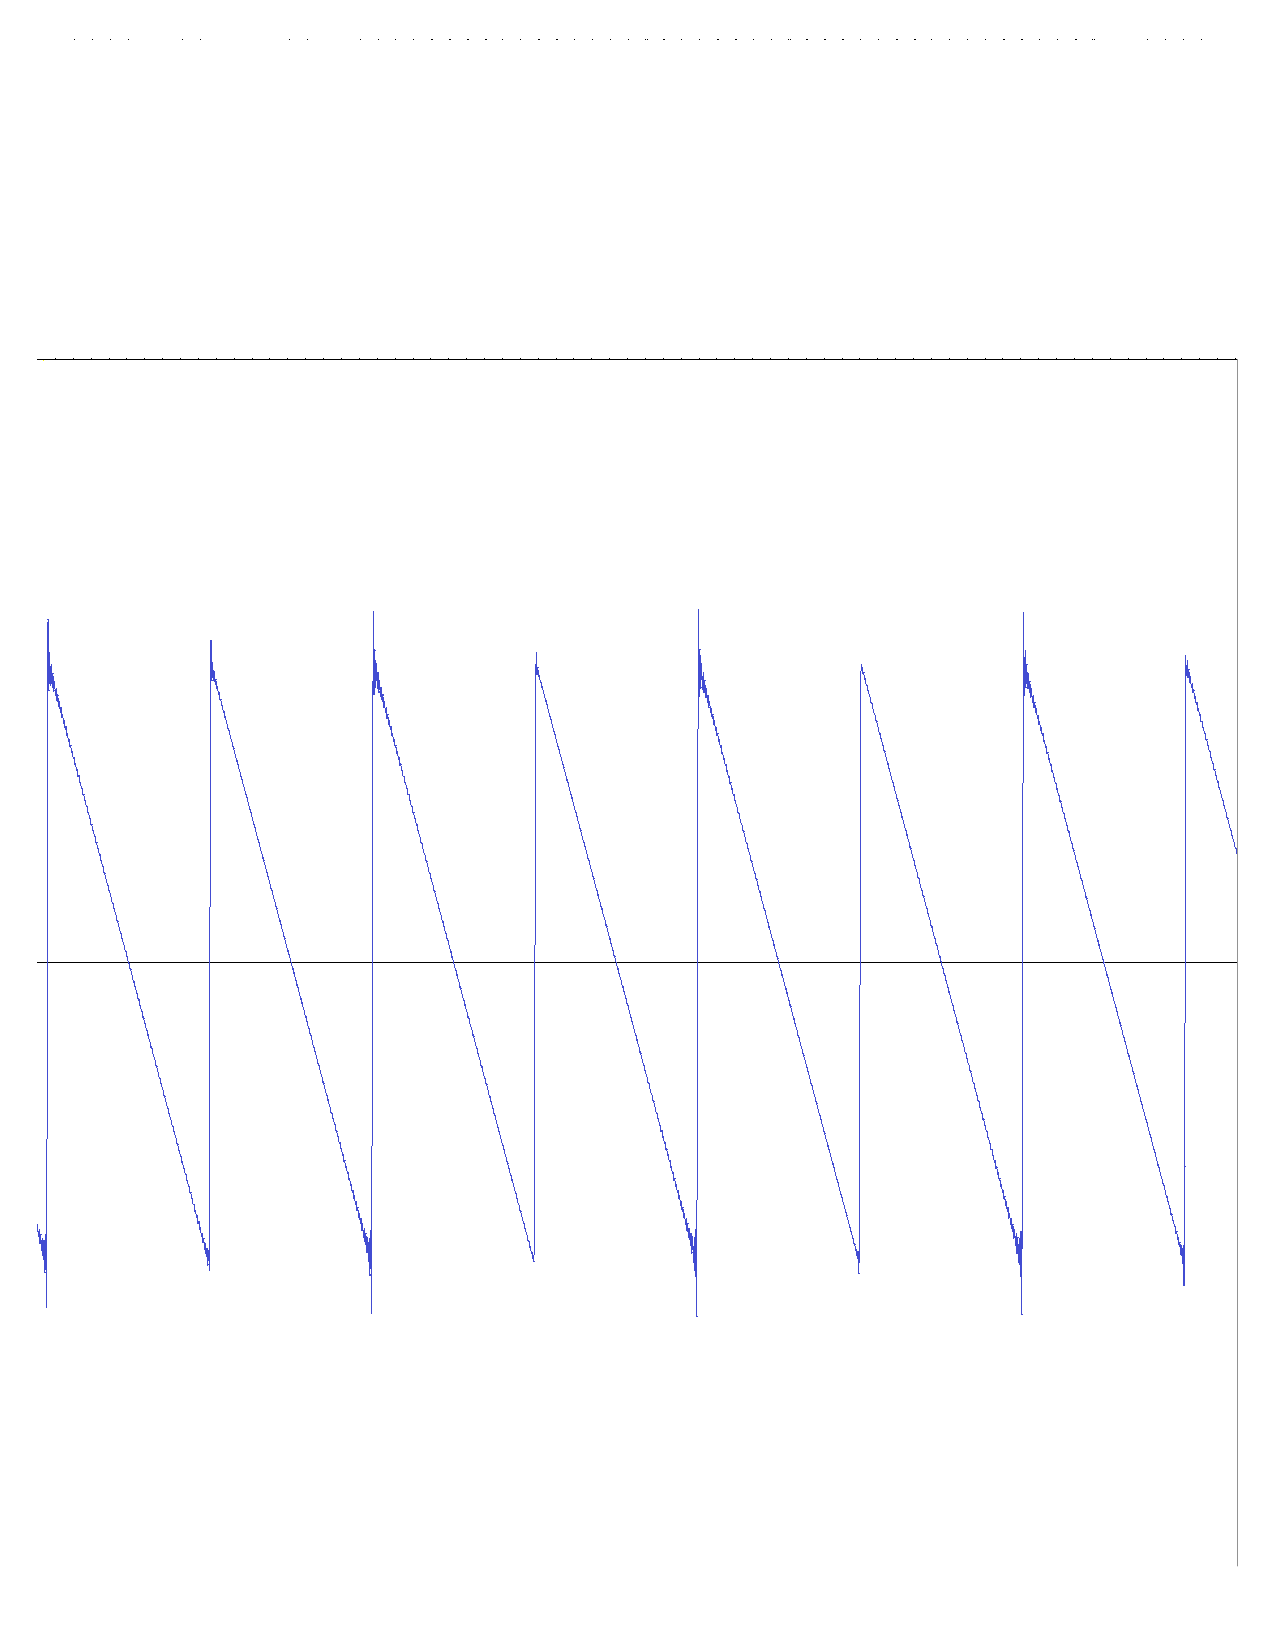
\includegraphics[trim=1cm 1cm 1cm 8cm, clip=true, width=1in, height=0.15in]{Saw1}}}\quad However this may sound too buzzy in low pitch sounds, so selecting this button will cause Flow to add a specific fixed set of random values to the phases of its partials.  This might change the Sawtooth wave to look like this \smash{\raisebox{-0.5em}{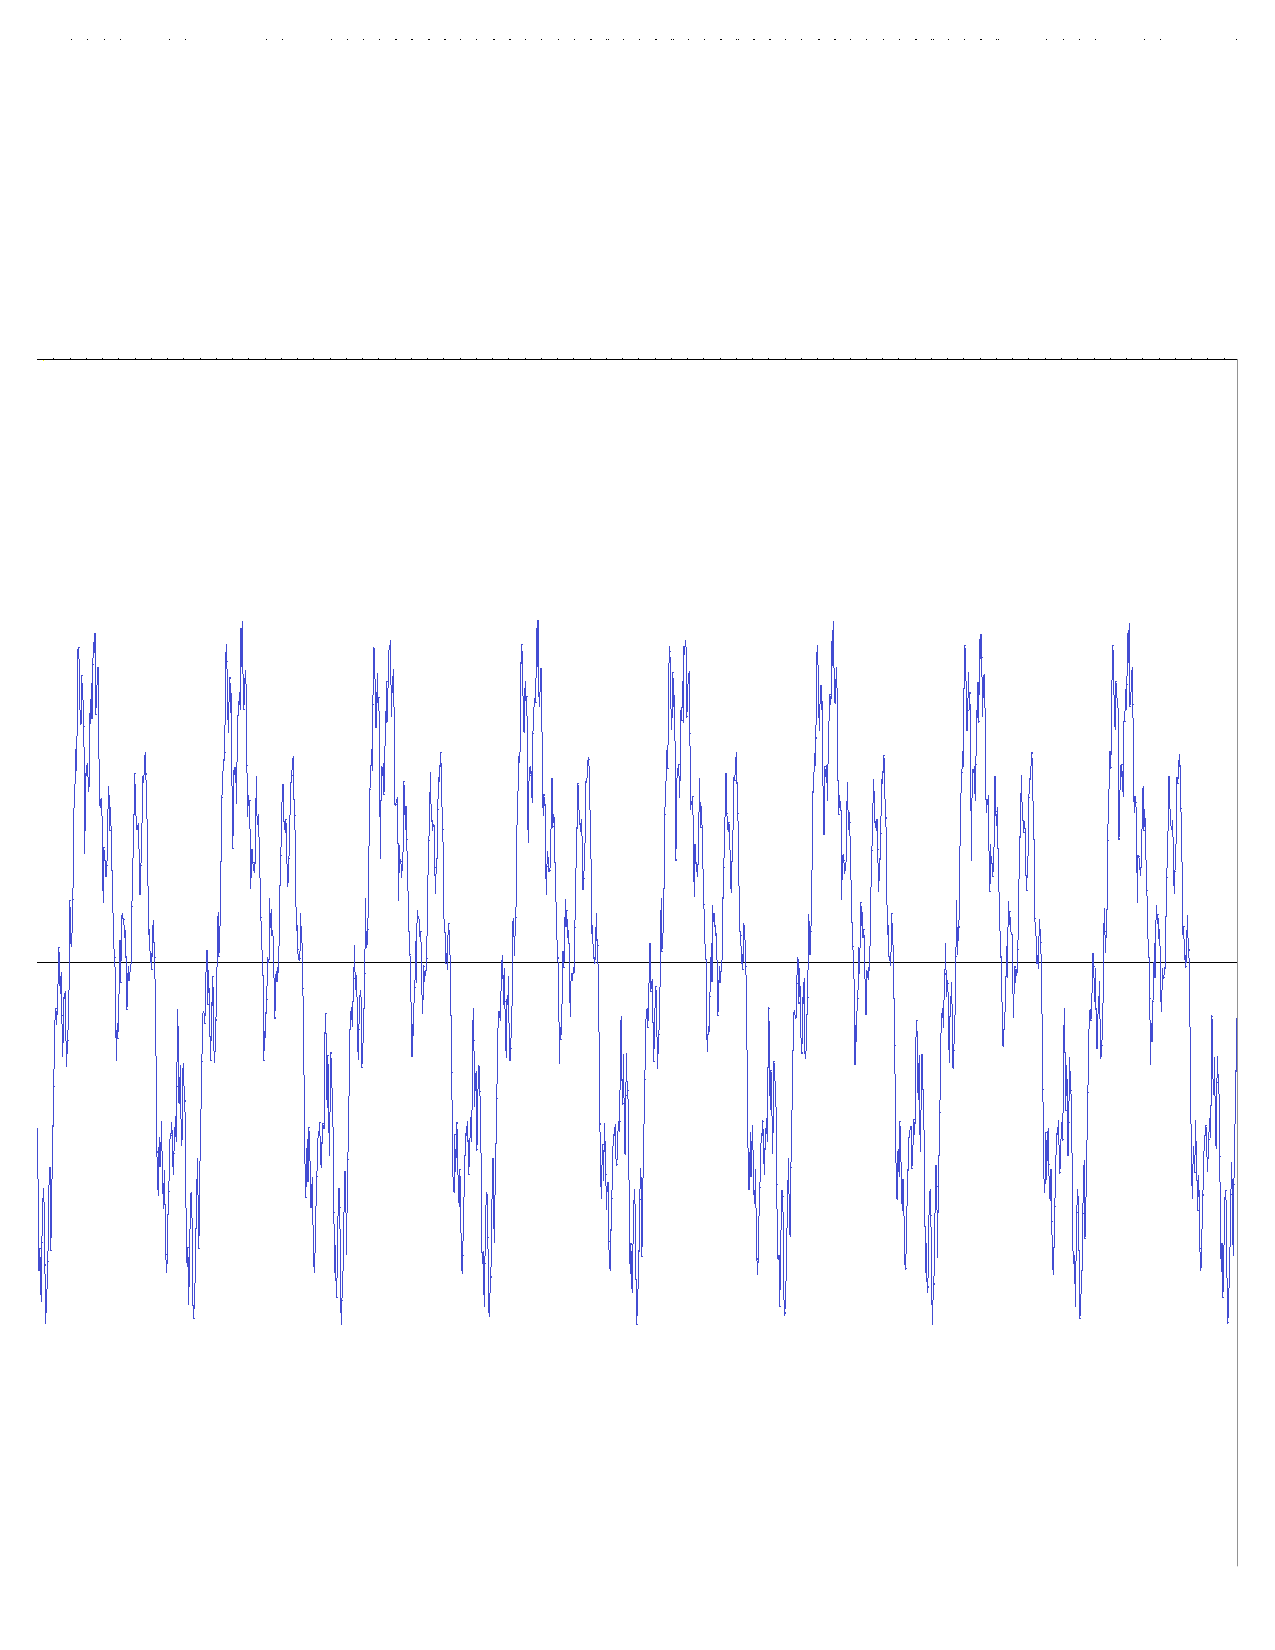
\includegraphics[trim=1cm 1cm 1cm 8cm, clip=true,width=1in, height=0.15in]{Saw2}}}\quad This sure doesn't {\it look} like a Sawtooth wave, but if you play it in the high- and mid- pitch notes, you'll find it {\it sounds} exactly the same!  For low-frequency notes the randomly-phased Sawtooth will sound less buzzy; you may or may not prefer this.  It {\it is} the case that randomly-phased sounds give Flow the opportunity to do some tricks which reduce computational cost by a bit.

\paragraph{Partials Visualization}  When you connect to the {\bf A} port, the resulting partials are also displayed on the left partials display in your rack.  The {\bf B} port is also useful for displaying partials (it shows them on the right partials display).  

The displays have certain special colors you should be aware of: the {\it Green} line is where your frequency 1.0 partial is located (if you have one!).  The {\it Blue} line, if displayed, shows the Nyquist limit: partials beyond this line are too high frequency to be represented in the digital sound signal and will be discarded.  Partials with zero amplitude are displayed in {\it Red}.  Similarly, partials with more than 1.0 amplitude are also displayed in {\it Red}.

\paragraph{Modulation Visualization} The Out module also lets you display modulation signals: the first two dials, normally labelled {\bf 1} and {\bf 2}, correspond to the left and right oscilloscope displays respectively.

In addition to the modulation signal, the oscilloscope also draws a helpful set of axes.  The color of these axes can be either {\it Blue} or {\it Green}: every time the signal produces a {\bf trigger}, the oscilloscope will change the color of the axes.

There's no reason you can't insert multiple Out modules into your patch: but only the last one will do anything.

\subsubsection{Creating a Macro with the \textit{In}, \textit{Out,} and \textit{Macro} Modules}
\label{creatingmacros}

Once you have saved your patch, you can reload it as a {\bf Macro} in a higher-level patch of your design: it will appear as a module like any other.  The partials fed into the ({\bf A}) port of your Out module, normally used to produce audio, will be available to feed into other modules. When used in a macro, Out's Reverb and Gain are disabled.  The underlying patch's information (author, etc.) are available by clicking on a disclosure triangle labelled {\it Info}.  Macro's outputs, like other partials shapers, can be constrained.

But that's not all.  Your patch can in fact output {\it four} partials streams, by default called {\bf A}, {\bf B}, {\bf C}, and {\bf D}.  And you can also output {\it four} modulation signals, called {\bf 1}, {\bf 2}, {\bf 3}, and {\bf 4}.  Just connect to them in the Out module of your original patch, and when you load it as a Macro, they're all available as outputs in the Macro module to feed into other modules. 

\paragraph{Input to a Macro: the \textit{In} Module}  So far so good.  But how about feeding partials and modulation signals {\it into} your Macro?  This is accomplished with the {\bf In} module.  The In module has four partials outputs and four modulation outputs, conveniently called {\bf A}, {\bf B}, {\bf C}, {\bf D}, {\bf 1}, {\bf 2}, {\bf 3}, and {\bf 4}, just like Out's input ports.  If, before you save your patch, you wire up some modules to listen in on these ports, then when you load the patch as a Macro, you can attach modules to feed into the Macro at those ports and their partials and modulation signals will be handed the modules inside the Macro.  Unlike Out, you can have as many In modules as you like: all of them will happily provide (the same) signals.

\paragraph{Modulation Defaults}

The In module also contains some modulation inputs (dials) with the same name as its modulation outputs.  The primary purpose of these inputs is to allow you to set default values for the Macro.   For example, if you set the first dial to 0.25, then the Macro will use 0.25 by default.  If while editing the patch you change these dials, then the In module will also temporarily send the same value out its equivalent modulation output.  This makes it a bit easier to figure out what values to set by default.  However this also means that you can also hook modulation signals to these inputs and the same signal will be output: but when you load the patch as a macro, these modulation signals will be ignored and the default will be set to 0.0.  In short: you should only set the dials manually, not via modulation signal: it'd be confusing otherwise.

\paragraph{Naming Things}

You can rename the input and output partials and modulation ports of your Macro.  This is accomplished by renaming their compatriots in your In and Out modules.  Note that, unlike in other modules, the ports in your In and Out modules have {\bf underlined labels}.  Just click on a label and you'll be asked to give it a new name.

Note that although you can have as many In modules as you like, and they will all work, only the ports of the first one will be used to rename ports in the Macro.  (Of course, as mentioned before, while you can have multiple Out modules, only the last one will function at all, and this includes naming ports).

\subsection{Mixing Strategies}
\label{mixingstrategies}

Ordinarily if you wanted to mix two sources into one stream, you'd imagine you could just lump all the partials together and be done with it.  But there are two catches.  First, {\name} has a fixed number of partials: so if you lump the partials from two sources together, half of them must be eliminated.  Second, partials are each associated with a sine wave oscillator in the output (that's the partial's {\it order}): when two sets of partials are mixed, you'll often have the situation where partials from each set are competing for that oscillator, and in the end only one can have it.  So it's a little more complex than you'd think.

{\name} has several modules which implement various strategies for mixing, depending on your needs: {\it Amp Math}, {\it Morph}, {\it Mix}, {\it Combine}, and {\it Fill}.  It's useful to understand how these strategies differ from one another.

First some terminology.  Let the two sets of partials from incoming partials be \(A\) and \(B\), and the resulting outputted by the mixing module be \(O\).   Sets of partials are actually arrays (lists).  Thus each partial has a {\it position} in the list: {\name} requires that lower-frequency partials have lower positions than higher-frequency partials.  Partial \(O_i\) is the \(i\)th partial in the list for output \(O\) (similarly \(A_i\) and \(B_i\)).  Each partial has an {\it amplitude}, a {\it frequency}, and an {\it order} (the oscillator ultimately used to output the partial).  We'll call these amp(\(O_i)\), freq(\(O_i\)), and ord(\(O_i\)) (and similarly for \(A\) and \(B\)).  The order is a unique integer but it's not the same thing as \(i\): as partials change their frequencies, they can get rearranged in a list but maintain their respective order tags.

\begin{itemize}
\item {\bf Amp Math} and {\bf Mix} both just line up the corresponding partials and perform a function on their amplitudes.  The frequencies of the first set of partials are used. That is, \(\text{amp}(O_i) = f(\text{amp}(A_i), \text{amp}(B_i))\) for some function \(f(...)\), but \(\text{freq}(O_i) = \text{freq}(A_i)\) and  \(\text{ord}(O_i) = \text{ord}(A_i)\).  

This can produce some surprises.  Let's say you made a sawtooth wave and detuned it in some way, then mixed it (as source B) with another plain old sawtooth.  All of your careful detuning will disappear!  This is because the frequencies of the outgoing partials are set to those of \(A\): in essence the partials of \(B\) will have their frequencies lined with \(A\) before the mix occurs.

\item {\bf Combine (non-``Half'')} throws all the partials from both sources together into a big bin, sorts them all by frequency (lowest to highest), then takes the lowest half, discarding the upper half.  If {\it Merge} is true, then if any partials have the exact same frequency, then they are unified into one partial: this means that potentially more than half of the total partials may be ultimately used.  

The big challenge with Combine is in the orders.  Combine allows all the partials originating from \(A\) to retain their original orders; then partials from \(B\) get to retain their orders if they're available (usually they're not); then the rest of the \(B\) partials are assigned new orders.  Reassigning the orders of partials is not a big problem: but if a partial changes its frequency relative to another, it's possible that its reassigned order may be abruptly changed.  This can cause a pop or buzz because the sine wave oscillator is being changed all of the sudden.  You might be able to help things by swapping Inputs A and B, or switching to the ``Half'' version of Combine (see below).

Combine (non-``Half'') works well for many things but not if you're mixing together a source with lots of high-frequency stuff plus a source with lots of low-frequency stuff, because only the low-frequency stuff will survive.  Instead, use ``Half'' in this case. 

\item {\bf Combine (``Half'')} cuts each of the incoming source partials in half (eliminating the highest frequency partials), then puts them together. This guarantees that each source has at least half of its partials in the final mix.  ``Half'' is not good if you want to mix one source with lots of partials with another source with only one or two partials.

\item {\bf Fill} adds to \(O\) all the non-zero amplitude partials of \(A\).  Any remaining partials come from the lowest non-zero partials of \(B\).  Fill is particularly useful when mixing in Noise from a limited number of partials: set \(A\) to the noise.  Fill also works great if both sources (or at least \(A\)) have lots of empty partials.  At present orders come from \(A\): orders in \(B\) are reassigned.  This could potentially create the same pop/buzz situation as discussed in Combine.

\item {\bf Morph} lines up partials in \(A\) and \(B\) according to some map and interpolates their frequencies and amplitudes.  Orders come from \(A\).  Because of interpolation, this is unlikely to create pops or buzzes in most situations.  



\end{itemize}

\bump
\section{Developing Modules}

\begin{wrapfigure}{r}{3.5in}
\vspace{-1em}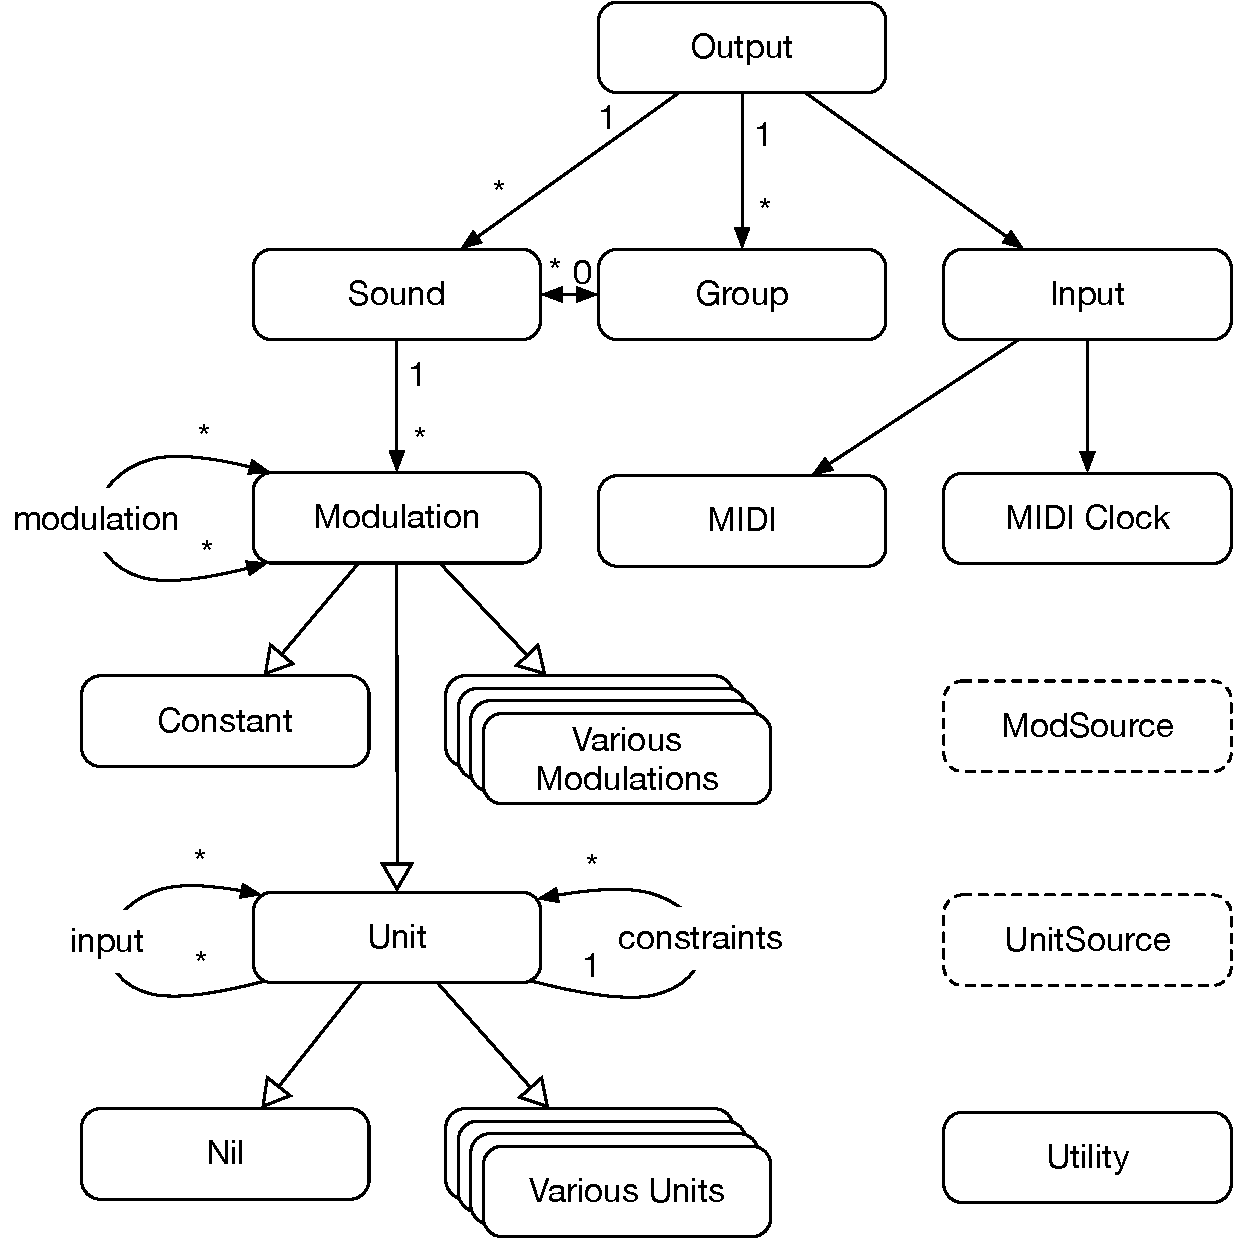
\includegraphics[width=3.5in]{CoreUML.pdf}
\vspace{-1em}
\caption{Core Classes.}
\vspace{-1em}
\end{wrapfigure}

The architecture behind {\name} is not particularly complex.  The top-level class, of which there is only a single instance, is {\bf Output}. This class is responsible for managing most of the threads in the system and for maintaining the facility which builds and emits samples to Java's audio system.  Output also contains a single {\bf Input} object which manages incoming MIDI data and sends it to the right places.  Input does this by working with {\bf MIDI}, an untidy class borrowed from Edisyn which provides a wrapper facility around Java's midi subsystem.

Critically, Output also contains some \(N\) {\bf Sound} objects, one per voice.  Sound objects are {\it registered} with Output.  Output, and not the Sound objects themselves, handles the spawning of voice threads associated with the Sound objects.  Each Sound object contains some number of {\it modules} which are attached to one another and pass partials or modulation signals to one another.  One module is designated as the module which {\it emits} a final set of partials to the Sound on request: Sounds then hand off their partials to the Output which uses them to produce samples to give to the audio system. 

Each Sound object belongs to a {\bf Group}, and there are up to \(G\) Groups stored in Output.   Each Group is really a patch (the Primary patch or a subpatch), and all Sounds associated with a Group have the same organization of module because the produce the same kind of sound.  Groups have names, MIDI channels, etc.  Each Group also has a user-requested number of voices (Sounds); the number of Sounds allocated to a Group will be no more than this number.  The Primary patch is Group 0, and it always contains at least one Sound (number 0).  Other Groups can have as few as zero Sounds.  You will rarely access a Sound's Group when developing a module.

The top-level abstract superclass for modules is {\bf Modulation}, which designates a module capable of receiving modulation signals from some \(M\) sources, and likewise some \(P\) different modulation signals which other modules may subscribe to.  A Modulation which the user will think of as primarily producing modulations, rather than filtering modulations, may be designated a {\bf ModSource}, which gives it a specific color in the GUI. Examples of ModSources might include LFOs or envelopes; though they do receive modulation (such as LFO's rate), their primary function is to provide modulation.  A Sample and Hold module, which receives an incoming signal and produces a stepped version of the same, would not be a ModSource.
 
Modulation signals are single numbers (ranging from 0...1) passed from module to module; these numbers typically change over time.  There are many Modulation subclasses, and you can create your own.  Generally Modulations are registered with Sounds, which will pulse them as necessary to produce timely modulation values.  But one special Modulation, {\bf Constant}, simply provides a single constant number all the time.  Constants are not registered with Sounds and primarily serve to fill in incoming modulation slots for which you do not have a Modulation class hooked up.  In the GUI, modulation dials which aren't wired to anything are represented by Constants.  {\tt null} cannot be used to fill an incoming modulation source slot: if it's not filled by some other Modulation, it must be filled by a Constant.

A special kind of Modulation is a {\bf Unit}.  This is the abstract superclass for modules which, in addition to (possibly) using and/or emitting modulation signals, also use and/or emit arrays of partials for additive synthesis.  Units provide timely partial arrays to other Units as necessary.  The module designated to {\it emit} partials to a Sound must be a Unit.  A Unit which primarily exists to produce partials may be designated to be a {\bf UnitSource} so as to give it a special recognizable color in the GUI.  A Unit which simply provides a Sawtooth wave is an example of a UnitSource; whereas a low-pass filter would not be.

A single partial consists of a real-valued {\it frequency} \(> 0\), a real-valued {\it amplitude} \(\geq 0\), and an integer (byte) tag called, confusingly, an {\it order}.  Frequencies are relative to a base pitch: thus the lowest frequency partial typically has a frequency of 1.0: this would normally be the {\it fundamental}.   However frequencies can be lower than this.  The {\it order} tag is a unique ID for this partial; when partials are moved around in the array, we can use the order tag to keep track of which partial is which. This is useful for some modules (notably {\it Smooth}), but it is particularly important when building the final sound, as each sine wave generator, and its current position in the sine wave, is based on the order.

Non-UnitSource Units typically filter or otherwise modify incoming partials from one or more sources and then send them on to other Units.  Before they sent them on, these Units typically will optionally {\it constrain} the partials by frequency.  This means that they will select some user-defined set of partials to reset back to the original values they held when they were received from the Unit's sources in the first place.  This allows the user, for example, to stipulate that he wants to apply a low-pass filter on all partials except the ones forming perfect fifths.  The user can also provide another Unit as a {\it constraint source}: the index numbers incoming partials for which it has nonzero amplitudes would indicate which partials the original Unit should preserve. 

Like Modulation, you can create your own Unit subclasses, and many already exist.  However one special Unit class is {\bf Nil}, which provides a single array of partials with zero-level amplitudes.  If a Unit's incoming partials source slot is not filled by another Unit, it will be filled by Nil. Source slots may not be {\tt null}.

The final class in the core package is {\bf Utility}, which simply provides various utility functions, notably mathematical approximations to various transcendental functions.

\begin{wrapfigure}{r}{2.5in}
\vspace{-1em}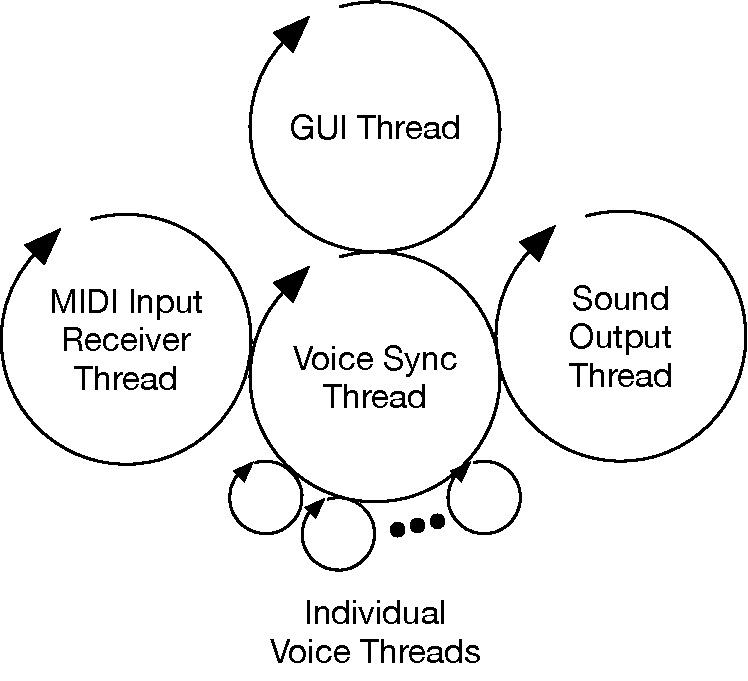
\includegraphics[width=2.5in]{Threads.pdf}
\vspace{-2em}
\caption{The threads and their interactions.}
\label{threads}
\end{wrapfigure}

\paragraph{Threads} These classes spawn and are manipulated by several threads, as shown in Figure~\ref{threads}.  First and foremost is the {\bf voice sync thread}.  This thread can either be spawned to run on its own, or it can simply be the application's \texttt{main(...)} thread, calling \texttt{output.go()} in an infinite loop.  The voice sync thread is responsible for getting the latest MIDI data from the {\bf MIDI input receiver thread}, then syncing all of the {\bf individual voice threads} and having them produce a new set of partials, one per Sound.  If there is only one voice, the voice sync thread has the option of handling that voice itself rather than spawning with and negotiating with an individual voice thread.  Finally, it hands these partials to the {\bf sound output thread} which converts them into a sound wave and emits it.  The sound output thread does this by splitting the task per-voice into separate output threads to add up the respective partials.

The sound output thread and MIDI input receiver threads run constantly in the background; but the voice sync thread and the individual voice threads can all be paused by locking on Output's {\bf sound lock}.  The recommended pattern is:\footnote{This isn't a synchronized statement because the lock is a ``fair'' (non-barging) recurrent lock internally.  The locks used in synchronized statements are (unfortunately) unfair, and we can't use that.}

\begin{verbatim}
Output output = ... ;
output.lock();
try
    {
    ... safely read or modify the Sounds and their various Modulations and Units here ...
    }
finally
    {
    output.unlock();
    }
\end{verbatim}

And indeed this is how the Swing event thread (if you have a GUI) interacts with the system: by acquiring the sound lock to read information to draw, or to modify things in response to GUI events.

\paragraph{When the threads are spawned}  The MIDI input receiver thread and the output sound thread are both spawned when you call {\tt new Output()}.  The voice sync thread is not necessarily spawned: if you call {\tt output.go()} in a tight loop, then you are the voice sync thread.  However you can spawn a voice sync thread to do this for you by calling {\tt output.startPrimaryVoiceThread()}.  The individual voice threads are spawned (if at all) as soon as the voice sync thread calls {\tt output.go()} for the first time.  This means that you must have constructed all the Sound objects and registered them with the Output prior to this happening.

\paragraph{Performance tuning parameters} You should be aware of several tunable parameters in Output.java which impact on the performance of these threads and ultimately the performance of the application.  Some of these are constants, others are variables which Output.java loads from Java preferences in its constructor, and are available to change in the GUI.

\begin{itemize}
\item {\tt SAMPLING\_RATE}\qquad This value, normally 44100, could of course be reduced (perhaps halved) to improve performance, but at a dramatic cost in sound quality.  I would not do that.

\item {\tt bufferSize}\qquad Specified by the user, by default, {\tt DEFAULT\_BUFFER\_SIZE} \(=1152\). The size of the sound buffer being fed by the sound output thread.  Java's audio system grabs data from this buffer in fairly random gulps: on the Mac they're 128 bytes at a time and can happen in spurts.  The sound output thread feeds the buffer two bytes (one 16-bit sample) at a time.  If the audio system cannot grab bytes from the buffer without reducing it to zero, then you will hear a {\bf glitch} (an audible pop or zap).  We don't want those.  We fix this by keeping the buffer pretty big.  The disadvantage of a large buffer is that if we have filled it, we're creating latency, and we don't want that either.  At an absolute minimum the buffer must be at least 1024 (the apparent minimum on the Mac to even work properly); but in reality we need it larger than that to prevent glitches.  1152 seems adequate but potentially can make a large latency (about 38 milliseconds worst-case).

\item {\tt SKIP}\qquad We don't necessarily produce a new set of partials for every single sample; if your computer isn't fast enough, this isn't reasonable.  Instead we generate \(N\) samples for each partials set.  This is the value of {\tt SKIP}.  The default value is 32.  Upon receiving a new sample set, the sound output thread linearly interpolates between the previous sample set and the next one over 32 samples.  This also induces a different kind of lag: if you generate a sound, you'll have to wait up to 32 samples before it begins to be produced, and up to 64 samples before it is fully present.  Ideally {\tt skip} would be 1, which would produce the best quality sound, as well as produce true FM synthesis effects.  But there you have it.

\item {\tt PARTIALS\_INTERPOLATION\_ALPHA}\qquad Because partials don't arrive every sample (see {\tt DEFAULT\_SKIP} above), we'd like to smoothly interpolate between them.  This is done by repeatedly multiplying in a small amount of the new partials amplitudes until they're dominant.  The amount multiplied in is {\tt PARTIALS\_INTERPOLATION\_ALPHA}, by default set to 0.05.  If you set this to a larger value, you'll start hearing pops or hisses when you make abrupt changes in volume in your partials (try a Drawbars patch to test).  But smaller values mean that new changes will take a longer time to take over\,---\,essentially a kind of attack rate.  At 0.05, partials are about 95\% takeover after about 100 samples (roughly three {\tt DEFAULT\_SKIP} intervals), or approximately 2ms, which seems reasonable.  At any rate, if you change {\tt DEFAULT\_SKIP}, this may have an impact on what setting you want to use for {\tt PARTIALS\_INTERPOLATION\_ALPHA} too.

\item {\tt numVoices}\qquad is the maximum number of voices that the system will generate.  Specified by the user, can be no more that {\tt MAX\_VOICES}. It is by default set to {\tt DEFAULT\_NUM\_VOICES} \(=8\).  More voices of course means more computing power required.

\item {\tt numVoicesPerThread}\qquad Specified by the user, by default {\tt DEFAULT\_NUM\_VOICES\_PER\_THREAD} \(=8\).  If you have a high thread context switching overhead, you can assign more than one voice to a single thread.  For example, if {\tt numVoicesPerThread} was equal to 2, then you'd have 4 threads handling your 8 voices.  If you don't have 8 cores, you might wish to do this.  However keep in mind that the total number of modules your voice can have is bounded by a single core: if you have two voices on a thread, they will share that core and your total number will be halved.

\item {\tt numOutputsPerThread}\qquad Specified by the user, by default {\tt DEFAULT\_NUM\_OUTPUTS\_PER\_THREAD} \(=2\).  Affects the number of output threads generated to convert the partial results into the sound.  Fewer threads, and you've got more work being done by a single processor (which may not be able to take the load); but more threads means more total work given the thread context switching.

\item {\tt MINIMUM\_VOLUME}\qquad If a sound is below this value, Flow doesn't bother adding it into the sum, which saves a little bit of CPU.

\end{itemize}

Finally, there's one constant in Unit.java of interest:

\begin{itemize}
\item {\tt NUM\_PARTIALS}\qquad is the number of partials being handed from module to module.  This is by default 128, but can be changed to 64 or 128 in the Preferences. 
\end{itemize}

\begin{figure}[t]
\begin{center}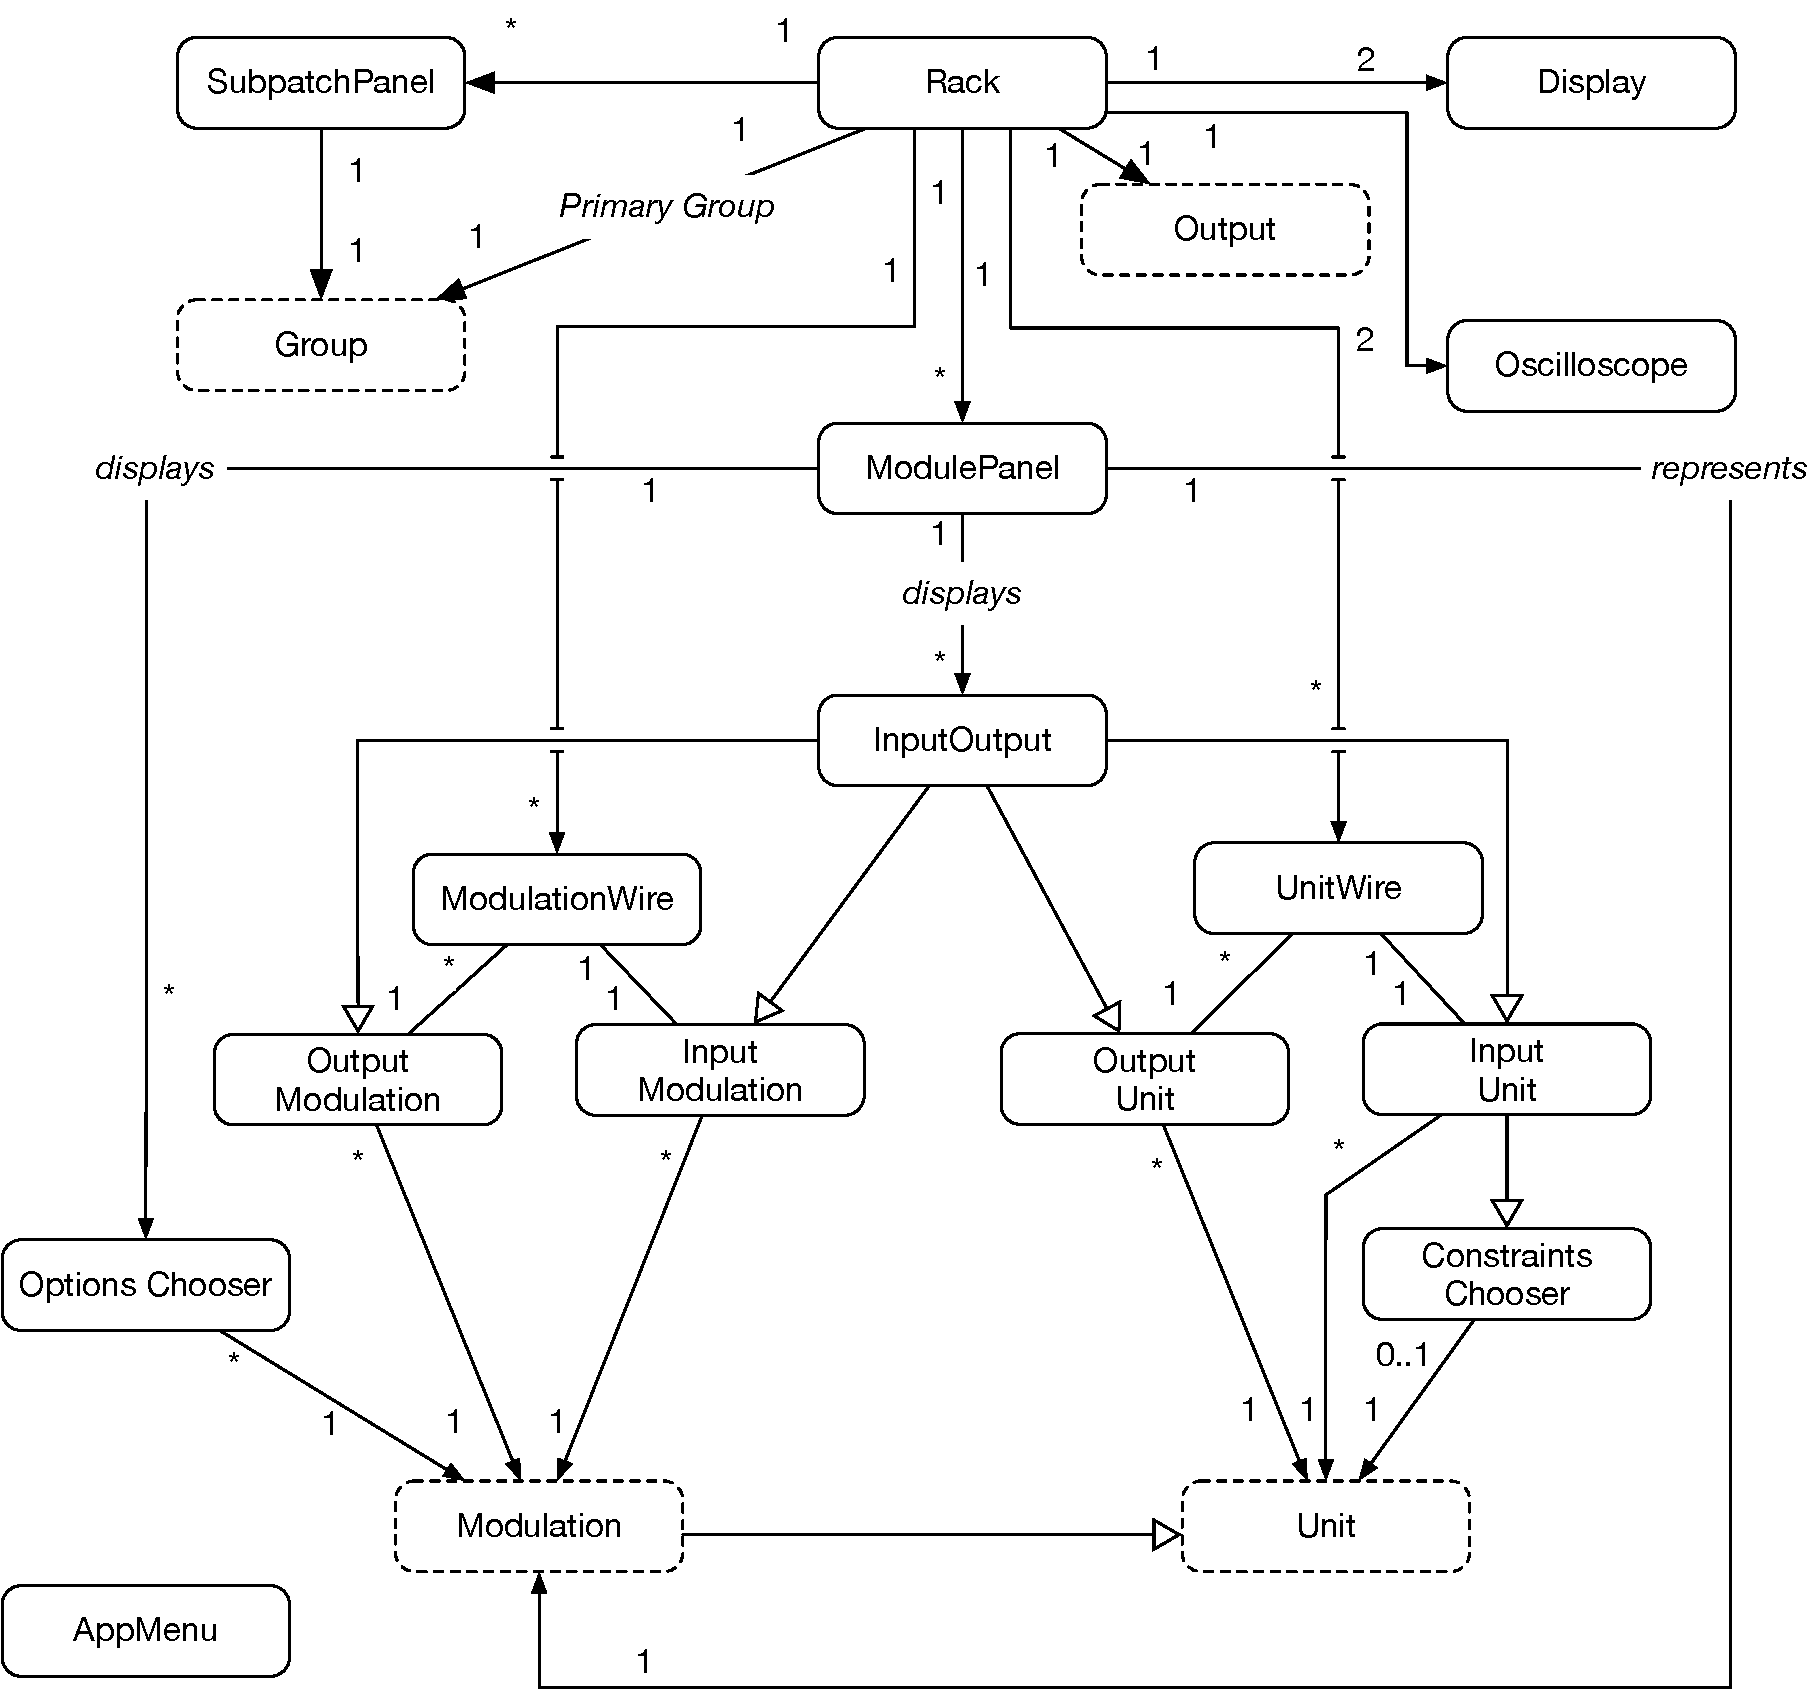
\includegraphics[width=5.3in]{GUIUML.pdf}\end{center}
\caption{The GUI Facility.}
\label{gui}
\end{figure}

\paragraph{The GUI} The GUI facility is (of course) structurally more complex than the core code, but it's not too bad: see Figure~\ref{gui}.  But here is the gist of it.  {\name} contains a single {\bf Rack} which is associated with the Output and which holds some \(N\) instances of {\bf ModulePanel} in a JScrollPane.  Each ModulePanel represents a {\it module} in the user's patch, either a Modulation or a Unit, and lets the user manipulate that module.  Recall that in fact there is one such module for every Sound: the ModulePanel will associate itself with the ``official'' copy of that module, namely the copy stored in Sound 0.

There are several parts of a module that the GUI must display to the user inside a ModulePanel:

\begin{itemize}
\item Ports for incoming Modulations to attach, or for the user to manipulate as if they were dials.  These are displayed using {\bf InputModulation}.
\item Ports for incoming Units to attach.  These are displayed using {\bf InputUnit}.
\item Ports to attach to outgoing Modulations.  These are displayed using {\bf OutputModulation}.
\item Ports to attach to outgoing Units.  These are displayed using {\bf OutputUnit}.
\item A {\bf ConstraintsChooser}.  This is the gizmo attached to ModulePanels for many (but not all) Units which allows you to constrain which partials are being modified.  It contains a combo box, a checkbox, and a port for an incoming Unit (which is why it's a subclass of InputUnit).
\item {\bf OptionsChoosers}.  These allow the user to select an option in a module: they're presented either as check boxes or combo boxes.
\end{itemize}

InputUnits, OutputUnits, InputModulations, and OutputModulations (and ConstraintsChoosers) share a lot of code in common, and so belong to a common abstract superclass called {\bf InputOutput}.  No, it's not a good name.

InputUnits and OutputUnits are connected together by the user with a {\bf UnitWire}.  Similarly, InputModulations and OutputModulations are connected together by the user with a {\bf ModulationWire}.

In addition to holding all ModulePanels, the Rack also holds the list of all InputWires and ModulationWires in in the patch.  The Rack also contains two {\bf Displays} which draw partials for the user.   The Rack is stored in a JFrame and is associated with the synth's menu.  The menu is produced via various static methods in {\bf AppMenu}.  AppMenu also stores the list of current available Modules (for now).

There are a few more utility GUI widget classes, but that's the bulk of it.

\paragraph{Macros and Patches}

The module {\bf Out} exists in practically every user patch, since it is the only way for them to produce a sound (for testing purposes you can produce sound with any Unit).  But besides producing sound, Out works with two other modules, {\bf In} and {\bf Macro}, to enable user macros.  It works like this. 

The user adds at least one Out and one In to his patch.  Out has several InputUnits (one of which is normally used to output sound) and InputModulations.  In has several OutputUnits and OutputModulations.  These InputOutputs are special: the user can edit their names.  The user can attach to these InputOutputs to provide input and output to the whole patch when it is used as a {\bf Macro}.    Then the user saves the patch (which just serializes out all the modules in the Rack).  The user can then load the patch as a Macro, at which point the all of the modules are put in a list managed by the Macro rather than by a Rack.  The original patch's Out module's InputUnits and InputModulations are attached directly to the Macro's OutputUnits and OutputModulations; and likewise, the In module's OutputUnits and OutputModulations are attached to the Macro's InputUnits and InputModulations.  Thus the whole patch becomes a module just like any other. 

Normally modules are registered with Sounds; but modules inside a Macro are not.  Instead the Macro is registered as a module with a Sound as usual, but when various event methods are called on it, it calls the equivalent on all of it subsidiary modules.  This process is recursive:\footnote{It's all down to your computational power.} Macros can contain Macros which contain Macros.


\subsection{Building a Modulation}
\label{buildlingamodulation}

A {\bf Modulation} is a module which emits modulation values.  It may also accept modulation values (ours will).  Let's make a trivial square wave generator.  Every \(N\) samples (at 44100 Hz) it will change from outputting a 0 to outputting a 1.  We'll add some more bells and whistles to it as we go along.  We start with a basic class:\footnote{Yes, the codebase is indented in Whitesmith's.  Resist the urge to burn it with fire.}

\vbox{\footnotesize
\begin{verbatim}
package flow.modules;
import flow.*;
public class MyModulation extends Modulation
    {
    public MyModulation(Sound sound)
        {
        super(sound);
        }
    
    public static String getName() { return "My Modulation"; }
    }
\end{verbatim}
}

The {\tt Sound} class defines the voice which owns the Modulation.  The call to {\tt super.sound()} is pretty critical, as it allows the Modulation to register itself with the voice in the first place.  The {\tt getName()} method is optional and tells {\name} what name to put in your module's title bar.  If you don't provide it (and many don't), the class name will be used.  Notice that the method is {\it static}.  It has to be.  A non-static version of this method will be ignored.  

\paragraph{Output Something}
Next let's output {\it something}, say 0.3:

\vbox{\footnotesize
\begin{verbatim}
package flow.modules;
import flow.*;
public class MyModulation extends Modulation
    {
    public MyModulation(Sound sound)
        {
        super(sound);
        }

    public void go()
        {
        super.go();
        setModulationOutput(0, 0.3);
        }
    
    public static String getName() { return "My Modulation"; }
    }
\end{verbatim}
}

The {\tt go()} method is pretty central.  It will be called whenever your module is being asked to update itself, by grabbing modulation and other information from elsewhere (if it needs to) and updating the modulation value it will output when asked to.  We are calling {\tt setModulationOutput(....)}, which tells the module to return 0.3 whenever someone connects to our output modulation port \#0 and calls {\tt modulate(\textit{port})} on it.  Be sure to call super.go().

\paragraph{Handle Time}
Next let's change our output values over time.

\vbox{\footnotesize
\begin{verbatim}
package flow.modules;
import flow.*;
public class MyModulation extends Modulation
    {
    int firstTick = --1;
    
    public MyModulation(Sound sound)
        {
        super(sound);
        }

    public void reset()
        {
        super.reset();
        firstTick = getSyncTick(true);
        }

    public void go()
        {
        super.go();
        if (firstTick < 0) return;
        int tick = getSyncTick(true);
        if (((tick / 44100) - firstTick) % 2 == 0)
            setModulationOutput(0, 0.0);
        else
            setModulationOutput(0, 1.0);
        }
    
    public static String getName() { return "My Modulation"; }
    }
\end{verbatim}
}

The method {\tt getSyncTick(true)} gives us the current {\it tick}.  This will be an integer value representing the number of samples that have been generated so far.\footnote{{\it getTick()} is currently a integer for threading efficiency reasons.  But this means it overflows after about 13 hours. We may change it to a long later.}  Here we're using it to switch from 0.0 to 1.0 every second.   Note that we pass {\it true} into {\tt getSyncTick(...)}: this tells Flow that if the MIDI clock is running, it should use the MIDI clock as the source of ticks rather than the wall clock.  Thus if the MIDI clock runs faster or slower, our ticks will come faster or slower as well.\footnote{If the MIDI clock is running as 120BPM, then the ticks from {\tt getSyncTick(...)} will be exactly the same as if we were using wall clock time.} 

The method {\it reset()} is called when our module is entirely reset.  We should override it to set ourselves to a pristine state.  Here this means grabbing the current tick and using that as our base for future timing.  Be sure to call {\tt super.reset()}.  As you can see, if {\tt firstTick} hasn't been set yet (it's -1), we don't update.

\paragraph{Handle Note-On}
Right now we have a {\bf free running} LFO of sorts: it changes from 0 to 1 regardless of what we're playing.  Instead let's it whenever we play a note.  Also, let's add in {\it another} modulation output, perhaps one which outputs the opposite of modulation \#0:

\vbox{\footnotesize
\begin{verbatim}
package flow.modules;
import flow.*;
public class MyModulation extends Modulation
    {
    int firstTick = -1;
    
    public MyModulation(Sound sound)
        {
        super(sound);
        defineModulationOutputs(new String[] { "Out", "Other" });
        }

    public void reset()
        {
        super.reset();
        firstTick = -1;
        }
        
    public void gate()
        {
        super.gate();
        firstTick = getSyncTick(true);
        }

    public void release()
        {
        super.release();
        if (!free) firstTick = -1;
        }

    public void go()
        {
        super.go();
        if (firstTick < 0) return;
        int tick = getSyncTick(true);
        if (((tick / 44100) - firstTick) % 2 == 0)
            setModulationOutput(0, 0.0);
        else
            setModulationOutput(0, 1.0);
        setModulationOutput(1, 1.0 - getModulationOutput(0));
        }
    
    public static String getName() { return "My Modulation"; }
    }
\end{verbatim}
}

What are we doing here?  Well first, we've added the method {\tt gate()}.  This method is called whenever a note is pressed (there's an equivalent method called {\tt release()} called when a note is released).  Here we're doing the same thing we used to do in {\tt reset()}.  As usual, be sure to call {\tt super.gate()}.  And now in {\tt reset()} we're just resetting the first tick to 0.

Additionally, in {\tt go()} we're setting output modulation port \#1 to be the opposite of what we just set in output modulation port \#0.  By default Modulation subclasses sport a single modulation port called ``Out''.  Because we now have two ports, we have to define them.  So we're doing that in our constructor.

\paragraph{Get Modulation from Elsewhere and Add Custom Options}
Next let's receive modulation from another source to define our modulation rate.  Additionally, we'll add two options, {\it free} (which determines whether our LFO is free) and {\it type} which adds unipolar options.

\vbox{\footnotesize
\begin{verbatim}
package flow.modules;
import flow.*;
public class MyModulation extends Modulation
    {
    int firstTick;
    boolean update;
    
    boolean free = false;
    public boolean getFree() { return free; }
    public void setFree(boolean val) { update = val; free = val; }
    
    public static final int TYPE_FULL = 0;
    public static int TYPE_UNIPOLAR_POSITIVE = 1;
    public static int TYPE_UNIPOLAR_NEGATIVE = 2;
    int type = TYPE_FULL;
    public int getType() { return type; }
    public void setType(int val) { type = val; }
    
    public MyModulation(Sound sound)
        {
        super(sound);
        defineModulationOutputs(new String[] { "Out", "Other" });
        defineModulations(new Constant[] { Constant.ONE }, new String { "Rate" });
        }

    public void reset()
        {
        super.reset();
        firstTick = getSyncTick(true);
        update = free;
        }
        
    public void gate()
        {
        super.gate();
        if (!free) update = true;
        }

    public void release()
        {
        super.release();
        if (!free) update = false;
        }

    public void go()
        {
        super.go();
        if (!update) return;
        double mod = modulate(0);
        int tick = getSyncTick(true);
        double val = 1.0;
        if (((int)((tick / (mod * 44099))) - firstTick + 1) % 2 == 0)   val = 0.0;
        if (type == TYPE_UNIPOLAR_POSITIVE)
            val = (val / 2.0) + 0.5;
        else if (type == TYPE_UNIPOLAR_NEGATIVE)
            val = (val / 2.0);
        setModulationOutput(0, val);
        setModulationOutput(1, 1.0 - val);
        }
    
    public static String getName() { return "My Modulation"; }
    }
\end{verbatim}
}

\clearpage

You'll notice that we've modified {\tt go()} to allow for building up the variable {\it val}, but you should be able to convince yourself that it's basically the same.  The first thing we do now is call {\tt modulate(0)}, which gives us the current modulation value of our modulation {\it input} port.  We then use this as a rate (notice that avoid dividing by zero: modulations go from 0.0 to 1.0 inclusive).  Finally, depending on whether we're currently unipolar, we may modify our value more.  We then set the modulation outputs to the value.

Notice also that we're now either resetting the tick in {\tt reset()} or in {\tt gate()} depending on the value of {\it free}; and we've {\tt release()} now to turn off a boolean called {\tt update} which we'll now use to determine whether to update the wave or not.

Since we're assuming a modulation input which defines our rate, we have to define it (modulations by default have no modulation inputs).  We do that in the constructor.  Notice that we provide not only a name for the input, but also an initial value.  Initial values are in the form of {\tt Constant} objects.   A Constant is a very simple Modulation which only outputs a single value between 0.0 and 1.0 and never changes unless you manually set it.  You can make your own Constant, or you could choose from one of several predefined ones in the {\tt Constant} class itself.  Here' we're choosing {\tt Constant.ONE}, which not surprisingly outputs a 1.0 (which will correspond to us using a rate of 44100).

\paragraph{Enable Custom Options in the GUI}
Currently our new {\it free} and {\it type} variables cannot be set by the GUI, but rather must be set programmatically.  We need to change that.  {\name} could have handled this with some elaborate manipulation of Java Reflection, but we have opted to go the simple route: by adding two general methods, {\tt getOptionValue(...)} and {\tt setOptionValue(...)}, which just call the appropriate methods internally for our {\bf options}.  We add the following code to our class:\footnote{Let's not replicate the class code over and over again any more: it's getting longer than a single page!}

\vbox{\footnotesize
\begin{verbatim}
    public static final int OPTION_FREE = 0;
    public static final int OPTION_TYPE = 1;

    public int getOptionValue(int option) 
        { 
        switch(option)
            {
            case OPTION_FREE: return getFree() ? 1 : 0;
            case OPTION_TYPE: return getType();
            default: throw new RuntimeException("No such option " + option);
            }
        }
  
    public void setOptionValue(int option, int value)
        { 
        switch(option)
            {
            case OPTION_FREE: setFree(value != 0); return;
            case OPTION_TYPE: setType(value); return;
            default: throw new RuntimeException("No such option " + option);
            }
        }
\end{verbatim}
}

Notice that since we have two options, we have two option values, 0 and 1.  All options accept and return integer values.  An boolean option (like {\it free}) should be mapped to the values 0 and 1, as we have done here.

In the GUI, {\name} will display boolean options as checkboxes, and non-boolean options as comboboxes.  But where does the GUI get the names for the options to display them?  Answer: we need to add a {\tt defineOptions(...)} method to the constructor.  We modify the constructor like this:

\vbox{\footnotesize
\begin{verbatim}
    public MyModulation(Sound sound)
        {
        super(sound);
        defineModulationOutputs(new String[] { "Out", "Other" });
        defineModulations(new Constant[] { Constant.ONE }, new String { "Rate" });
        defineOptions(new String[] { "Free", "Type" }, 
                      new String[][] { { "Free" }, { "Full", "Unipolar", "Negative Unipolar" } } );
        }
\end{verbatim}
}

The method {\tt defineOptions(...)} takes two arguments: an array of names for the options, and an array of arrays of names for possible values the options can take on.  But if an option is boolean, and is being displayed as a checkbox, then what are its ``option values''?  {\tt defineOptions(...)} will treat any method with {\it zero} or {\it one} option values, or a null option values array, as a boolean option.  The checkbox label will be the option name, not the option value.  We could have put an empty String array there, or null, but modules normally stick a single String there, the same as the option name.  So here, by adding the single option name ``Free'', with a single option value String, we have defined a checkbox which will simply say ``Free''.

The other option, ``Type'', will be displayed as a combobox with three options, ``Full'', ``Unipolar'', and ``Negative Unipolar'', representing values 0, 1, and 2 respectively. The title of the box will be ``Type''.  Note that ``Negative Unipolar'' is quite long, resulting in a long combobox and a thick module panel\,---\,and wasted space.  You might want to think about how to shorten names as much as possible.

\paragraph{Add Triggers}
Let's add a {\bf trigger} to our Modulation.  Every time we transition from low to high, we want to also set a trigger.  Attached modules can detect this trigger and use it to pulse themselves.  We modify the {\tt go()} method as follows:

\vbox{\footnotesize
\begin{verbatim}
    boolean transitioned = false;
    public void go()
        {
        super.go();
        if (!update) return;
        double mod = modulate(0);
        int tick = getSyncTick(true);
        double val = 1.0;
        if (((int)((tick / (mod * 44099))) - firstTick + 1) % 2 == 0)
            {
            val = 0.0;
            transitioned = false;
            }
        else
            {
            val = 1.0;
            if (!transitioned)
                {
                setTrigger(0);
                transitioned = true;
                }
            }
        if (type == TYPE_UNIPOLAR_POSITIVE)
            val = (val / 2.0) + 0.5;
        else if (type == TYPE_UNIPOLAR_NEGATIVE)
            val = (val / 2.0);
        setModulationOutput(0, val);
        setModulationOutput(1, 1.0 - val);
      }
\end{verbatim}
}

We want our trigger to happen only when we transition high.  So notice that when we transition to 1.0, we set the trigger only if it's not been set since the last transition to 0.0 (where we reset things). 

When we call {\tt setTrigger(0)}, this sets the trigger in outgoing modulation port 0.  Why don't we clear it?  Because a trigger only occurs for one tick.  Inside {\tt super.go()} it'll automatically clear all triggers next time.

\paragraph{Add Presets}
Let's finish out by adding some presets.  Modulations (and Units) which permit Presets implement the {\tt Presetable} interface.\footnote{I don't know if this should be Presettable or Presetable.  The latter is shorter though.}  So we'll change our class declaration as:

\vbox{\footnotesize
\begin{verbatim}
public class MyModulation extends Modulation implements Presetable
\end{verbatim}
}

To implement this method we need to create two new methods.  The first gives our list of presets, and the second responds when the user has chosen one.

\vbox{\footnotesize
\begin{verbatim}
public String[] getPresets()
    {
    return new String[] { "Free and Full", "Not Free and Positive" }; 
    }

public void setPreset(int preset) 
    {
    if (preset == 0) // free and full!
        {
        setFree(true);
        setType(TYPE_FULL);
        }
    else if (preset == 1) // not free and positive!
        {
        setFree(false);
        setType(TYPE_UNIPOLAR_POSITIVE);
        }
    }
\end{verbatim}
}

That should do the job.  Of course, you might want to make a table of preset values and names instead of doing it this way.  But there you go.

\paragraph{Test the Code}
Now let's try it out.  Run Flow as:

\vbox{\footnotesize
\begin{verbatim}
java -Dmodule=flow.modules.MyModulation flow.Flow
\end{verbatim}
}
... and the MyModulation module should appear as a modulation in the menu.  Later you can make this permanent by adding the  {\tt flow.modules.MyModulation.class} class to the list of modules called {\tt static final Class[] modules} in 
 {\tt additive/gui/AppMenu.java}.  
 
 Now create an empty patch, add an {\bf Out} and a {\bf MyModulation} to it, and hook up our {\it out} and {\it other} ports to Out's {\it 1} and {\it 2} dials.  Check ``free'', and you should start seeing stuff on the oscilloscopes.  Change the rate and see what happens.
 
There's one oddity: the title bar is pink, and it appeared in the ``Modulation Shapers'' menu, not the ``Modulation Sources'' menu.  This is because {\name} thinks that MyModulation is meant to revise or filter an incoming Modulation.  But of course it's not; MyModulation really is a modulation source.  Why does {\name} think this?  Because MyModulation has a modulation input port.  We can clue {\name} in by modifying MyModulation's class declaration as:

\vbox{\footnotesize
\begin{verbatim}
public class MyModulation extends Modulation implements Presetable, ModSource
\end{verbatim}
}

{\tt ModSource} simply tells {\name} that MyModulation is a modulation source, not some kind of modulation shaping thing.  Now it's in the right menu and the right title bar color.

\paragraph{Saving and Loading Patches}

Flow saves and loads patches to very simple files: they're just GZipped JSON text files.   Typically your module will load and save without any issue.  However you should be aware of some items.

First: there is a special optional JSON object available for you if you need to save custom data.  It's accessed by overriding the methods {\tt getData()} and {\tt setData(...)}.  See Wavetable and Draw for examples.

Second: the key for each modulation input/output, each unit input/output, and each option in your module is a string which is normally just the title of the item.  For example, the key for our ModulationOutput entitled {\it Other} is simply {\tt "Other"}.  This can be a problem if you have elements of the same kind (ModulationOutputs say) which have the same name, or a name which changes.  For example, the Envelope module has a bunch of modulation inputs all called {\it Level}.  To deal with this you can override the method {\tt getKeyForModulationOutput(...)} (or {\it getKeyForOption(...), etc.}) to return a designated unique key.

Third: you might also change your module, which causes problems when trying to be backward-compatible during loading.  If you update your module, you might override your modulation version in {\tt getVersion(...)}.  If you've changed your options, modulation inputs/outputs, and unit inputs/outputs, perhaps adding a new one or deleting some, you might need to check for this immediately before and/or immediately after they are loaded and set automatically, so as to revise them.  The methods {\tt preprocessLoad(...)} and {\tt postprocessLoad(...)} may be helpful.  You could completely override everything, if you wanted, by overriding the methods {\tt loadModulations(...)} or {\tt loadOptions(...)} etc..   Or you could just override {\t load(...)}.

\paragraph{The Current Patch Format}  The format is in GZipped JSON and is as follows:

\begin{itemize}
\item {\tt \{  "flow":{\it flow-version}, "name":{\it patch-name}, "by":{\it patch-author}, "on":{\it patch-date}, \rule[0in]{0in}{0in}~\hspace{\fill}\hbox{ "info":{\it patch-info}, "v":{\it patch-version},}  "modules":{\it modules}, "sub":{\it optional-subpatches} \} }
\item {\it flow-version:}\quad an integer \(\geq 0\) indicating the version of Flow which created this file.  Presently 0. 
\item {\it patch-name:}\quad The name of the patch, as stipulated by the patch creator.  A string. 
\item {\it patch-author:}\quad The patch creator.  A string.  
\item {\it patch-date:}\quad The patch creation date.  A string.  
\item {\it patch-info:}\quad Useful information about the patch, as stipulated by the patch creator.  A string.  
\item {\it patch-version:}\quad The version of the patch, as stipulated by the patch creator.  A string. 
\item {\it modules:}\quad {\tt [ {\it module,*} ] }
\item {\it module:}\quad {\tt \{ "v":{\it module-version}, "class":{\it module-classname}, "id":{\it module-id}, "opt":{\it options}, \rule[0in]{0in}{0in}~\hspace{\fill} "unit":{\it unit-inputs}, "mod":{\it modulation-inputs}, {\it optional-constraints}, {\it optional-data} \}}
\item {\it module-version:}\quad the version of this kind of module.  An integer \(\geq 0\).  Modules are presently largely at 0.
\item {\it module-classname:}\quad the class name of this module.  A string.
\item {\it id:}\quad A unique identifier of this module, which is referenced by other modules when they state that they are connected to it.  A string.
\item {\it optional-constraints:}\quad A JSON object in the form:\quad {\tt "constrain":\{~"id"={\it id }, "at"={\it modulation-unit-name}, "type"={\it constraints-type}, "not"={\it constraints-inverse}~\}}\quad  This object does not need to appear in the patch at all.  Additionally, all of the elements inside the patch are optional: they may appear or they may not, except that {\tt "id"} and {\tt "at"} must appear together.
\item {\it constraints-type:}\quad The value of the constraints type (an integer).
\item {\it constraints-inverse:}\quad Whether or not the options is inversed (a boolean).
\item {\it optional-data:}\quad A JSON object in the form {\tt "data":\{...\}} which the module may use as it likes to store additional data.  This object does not need to appear in the patch at all.  See Wavetable and Draw for examples of usage of optional data.  Additionally, both the In and Out modules use optional-data to store the user-defined names for their modulations and units (as an array of Strings called {\tt "mod"} and another array of Strings called {\tt "unit"}).
\item {\it options:}\quad {\tt \{ {\it option-name}:{\it option-value,*} \}}
\item {\it option-name:}\quad An option name (a string).  Normally this is the same as returned by {\tt getOptionName(...)}.
\item {\it option-value:}\quad The value of the option (an integer). 
\item {\it modulation-inputs:}\quad {\tt \{ {\it modulation-input-name}:{\it modulation-input,*} \}}
\item {\it modulation-input-name:}\quad A modulation input name (a string).  Normally this is the same as returned by {\tt getModulationName(...)}.
\item {\it modulation-input-value:}\quad Either a double between 0.0 or 1.0 representing the modulation dial value, or a {\it modulation-output}. 
\item {\it modulation-output:}\quad {\tt \{ "at":{\it modulation-output-name}, "id":{\it id} \}}\qquad The id is for the attached module.
\item {\it modulation-output-name:}\quad A modulation output name (a string).  Normally this is the same as returned by {\tt getModulationOutputName(...)}.
\item {\it unit-inputs:}\quad {\tt \{ {\it unit-input-name}:{\it unit-input,*} \}}
\item {\it unit-input-name:}\quad A unit input name (a string).  Normally this is the same as returned by {\tt getInputName(...)}.
\item {\it unit-input-value:}\quad{\tt \{ "at":{\it unit-output-name}, "id":{\it id} \}}\qquad The id is for the attached module.
\item {\it unit-output-name:}\quad A unit output name (a string).  Normally this is the same as returned by {\tt getOutputName(...)}.
\item {\it optional-subpatches:}\quad {\tt [ {\it subpatch,*} ] }
\item {\it subpatch:}\quad {\tt \{ "voices":{\it subpatch-voices}, "gain":{\it subpatch-gain}, "note": {\it optional-subpach-note}, \\
\rule[0in]{0in}{0in}~\hspace{\fill}\hbox{"midi":{\it optional-subpatch-midi-channel},  "flow":{\it flow-version}, "name":{\it patch-name},} \\ 
\rule[0in]{0in}{0in}~\hspace{\fill}\hbox{"by":{\it patch-author}, "on":{\it patch-date}, "info":{\it patch-info}, "v":{\it patch-version},}
 "modules":{\it modules} \} }
\item {\it subpatch-voices:}\quad The requested number of voices (Sounds) for this subpatch (an integer).
\item {\it subpatch-gain:}\quad The requested gain for this subpatch (a double).
\item {\it optional-subpatch-midi-channel:}\quad The subpatch's midi channel, 0--16.  0, or missing, means ``No channel''. 
\item {\it optional-subpatch-midi-channel:}\quad The MIDI note for the subpath, 0--128.  0, or missing, means ``Any note''.  Otherwise the note is the value, minus 1.
\end{itemize}

\paragraph{Cloning}  One obscure feature of {\name} is that Modulations and Units can not just be {\it moved} in the Rack, but can in fact be {\it copied}.  This is done by holding the Control key (on the Mac, Option also works) while dragging the Module.  This in turn calls the Module's {\tt clone()} method.  You need to override this method to insure that it performs a deep clone.  In many situations you'd need not implement this method at all.  But if your Modulation or Unit is holding an array or perhaps some other object which must be copied, you'll need to implement it like this:

\vbox{\footnotesize
\begin{verbatim}
     int[] stuff;    // let's say this is the array you need to copy into the cloned object
     public Object clone()
        {
        MyClass obj = (MyClass)(super.clone());
        obj.stuff = (int[])(stuff.clone());
        return obj;
        }
\end{verbatim}
}

\subsection{Building a Unit}

Read Section \ref{buildlingamodulation} (Building a Modulation) first.  It covers a lot of important stuff that we'll build on here.

A {\bf Unit} is a module which emits partials.  If you like, it can also accept partials, and can both accept and emit modulations.  Let's make a trivial low pass filter: we'll zero out the amplitude of a partial if the partial is less than a certain value, which we'll define as a modulation.

We begin by making a Unit subclass.  Note that Unit is a subclass of Modulation, so we're also making a Modulation.  However, while Modulations by default have one modulation output defined (``Out''), Units have zero defined by default.   They do, however, have one partials output defined (also called ``Out'').

\vbox{\footnotesize
\begin{verbatim}
package flow.modules;
import flow.*;
public class MyUnit extends Unit
    {
    public MyUnit(Sound sound)
        {
        super(sound);
        defineModulations(new Constant[] { Constant.HALF }, new String { "Cutoff" });
        defineInputs(new Unit[] { Unit.NIL }, new String { "In" });
        }
 
     public void go()
        {
        super.go();
        double mod = modulate(0);

        pushFrequencies(0);
        copyAmplitudes(0);
                        
        double[] amplitudes = getAmplitudes(0);
        double[] frequencies = getFrequencies(0);
                
        // we'll do more here...
        }
      }
   
    public static String getName() { return "My Unit"; }
    }
\end{verbatim}
}

We define one modulation input called ``Cutoff'', and set up {\tt go}.   Since we're receiving partials, we define one incoming partials port, called {\it In}.  By default the source module for this port is {\tt Unit.NIL}, which represents the ``empty Unit'', with standardized frequencies and all-zero amplitudes.    You can't use {\tt null} here: every partials input must be a real Unit.  When the user wires up the port to some other module, {\tt Unit.NIL} will be replaced with that module's output.

It's important to understand what the {\tt pushFrequencies(0)} and {\tt copyAmplitudes(0)} lines are doing.  {\tt pushFrequencies(input, output)} instructs the module to set the frequencies of all partials in output port {\it output} to those in input port {\it input}.  Because in the large majority of cases we don't have more than one partials output,   {\tt pushFrequencies(input)} does the same thing as  {\tt pushFrequencies(input, 0)}.  If you have pushed your frequencies (or your amplitudes), you may read them but you {\bf may not modify them}.  You'd push frequencies or amplitudes if you're not modifying them, because pushing is more efficient than copying them.

Because we're modifying amplitudes, we call {\tt copyAmplitudes(0)} instead of {\tt pushAmplitudes(0)}.  The method {\tt copyAmplitudes(input, output)} makes a copy of the amplitudes from {\it input} and puts the copy in {\it output}.  And similarly, {\tt copyAmplitudes(input)} is just {\tt copyAmplitudes(input, 0)}.

So what are the amplitudes and frequencies of our partials? They are each an array, normally of length 128, of doubles.  Both amplitudes and frequencies must be \(\geq 0\).  We extract the current amplitudes and frequencies from output port 0 with {\tt getAmplitudes(0)} and {\tt getFrequencies(0)} respectively.  Remember that the extracted frequencies are {\bf not to be modified} because we pushed them.

Notice that we've said nothing about the Orders.  This is because changing Orders is so rare that they're pushed automatically for you in {\tt super.go()}.\footnote{If for some reason you do {\it not} want this behavior, then in your constructor you should call {\tt setPushOrders(false);} and be sure to copy or push the orders yourself manually in your {\tt go()} method.}

\paragraph{Do the Filter} 
Next let's determine our cutoff frequency and do some cutting-off!

\vbox{\footnotesize
\begin{verbatim}
package flow.modules;
import flow.*;
public class MyUnit extends Unit
    {
    public MyUnit(Sound sound)
        {
        super(sound);
        defineModulations(new Constant[] { Constant.HALF }, new String { "Cutoff" });
        defineInputs(new Unit[] { Unit.NIL }, new String { "In" });
        }
 
     public void go()
        {
        super.go();
        double mod = modulate(0);
        double cutoff = modToFrequency(mod);
        double pitch = getSound().getPitch();
        
        pushFrequencies(0);
        copyAmplitudes(0);
                        
        double[] amplitudes = getAmplitudes(0);
        double[] frequencies = getFrequencies(0);    
        
        for(int i = 0; i < amplitudes.length; i++)
            {
            if (frequencies[i] * pitch > cutoff)
                amplitudes[i] = 0;
            }
        }
      }
   
    public static String getName() { return "My Unit"; }
    }
\end{verbatim}
}

Now we're cooking!  We just do a for-loop over the amplitudes and zero them if the corresponding frequency is too high.  But notice the usage of {\it pitch}.  Frequencies in partials aren't absolute frequencies: they're multiples of the pitch frequency of the current note (which typically, but not always, corresponds to the frequency of the fundamental).  So if we want to get the true frequency of a partial, we have to multiply it by the pitch.  The pitch is extracted from the module's {\bf Sound}, that is, the voice it's assigned to.  Sounds have a number of items they can provide: pitch is one of them.

Now, modulation values go from 0...1.  How do we convert that into a frequency?  We could just multiply by half the sampling rate (remember that anything over half the sampling rate is beyond the Nyquist limit), that is, something like \hbox{\tt cutoff = mod * Output.SAMPLING\_RATE}\quad But frequency is exponential, so we'd like something exponential-ish.  That's what the Modulation utility method {\tt modToFrequency(...)} does.  You might prefer it, or not.

\paragraph{Add Trigger Response} 
Now let's throw in a monkey wrench.  Imagine that we'd like to swap between low-pass and high-pass depending on the state of a trigger sent to us, oh, let's say, the Modulation we just developed in Section~\ref{buildlingamodulation}.   We might write:


\vbox{\footnotesize
\begin{verbatim}
package flow.modules;
import flow.*;
public class MyUnit extends Unit
    {
    boolean lowpass;
    
    public MyUnit(Sound sound)
        {
        super(sound);
        defineModulations(new Constant[] { Constant.HALF, Constant.ZERO }, new String { "Cutoff", "Trigger" });
        defineInputs(new Unit[] { Unit.NIL }, new String { "In" });
        }

     public void reset()
          {
          super.reset();
          lowpass = true;
          }
          
    public void gate()
          {
          super.gate();
          lowpass = true;
          }
          
    public void go()
          {
          super.go();
          double mod = modulate(0);
          double cutoff = modToFrequency(mod);
          double pitch = getSound().getPitch();
        
          pushFrequencies(0);
          copyAmplitudes(0);
                        
          double[] amplitudes = getAmplitudes(0);
          double[] frequencies = getFrequencies(0);    
        
          if (isTriggered(1)) lowpass = !lowpass;
          for(int i = 0; i < amplitudes.length; i++)
               {
               if ((lowpass && frequencies[i] * pitch > cutoff) || (!lowpass && frequencies[i] * pitch <= cutoff))
                    amplitudes[i] = 0;
               }
          }
     }
   
    public static String getName() { return "My Unit"; }
    }
\end{verbatim}
}

We created a boolean variable, {\tt lowpass}, to toggle between a low-pass and high-pass filter. In {\tt reset()} and {\tt gate()} we set {\tt lowpass} to true.  Next, we added an additional modulation for the trigger.  To get this trigger information, we call {\tt isTriggered(input)}.  There also exists a method called {\tt getTrigger(input)} which returns the {\it count} of how many times the trigger has been fired.  Finally, we use the trigger to toggle between low-pass and high-pass.  Recall that the trigger is reset the next iteration.

\paragraph{Add Constraints} 
One item many filter-style Units have is a {\it constraints facility}.  This is a facility that the user can use to restrict which partials we're allowed to modify.  In fact we'll modify all of them anyway, but then the constraints facility will restore some of them.  The method that does this is called {\tt constrain()}.  We modify {\tt go()} thusly:

\vbox{\footnotesize
\begin{verbatim}
    public void go()
          {
          super.go();
          double mod = modulate(0);
          double cutoff = modToFrequency(mod);
          double pitch = getSound().getPitch();
        
          pushFrequencies(0);
          copyAmplitudes(0);
                        
          double[] amplitudes = getAmplitudes(0);
          double[] frequencies = getFrequencies(0);    
        
          if (isTriggered(1)) lowpass = !lowpass;
          for(int i = 0; i < amplitudes.length; i++)
               {
               if ((lowpass && frequencies[i] * pitch > cutoff) || (!lowpass && frequencies[i] * pitch <= cutoff))
                    amplitudes[i] = 0;
               }
               
          constrain();
          }
\end{verbatim}
}

That's it!  We're constrained.  Because constraints are so common for filter-style Units, the GUI for them is added automatically.  If you don't want constraints for some reason, you turn them off by overriding the method {\tt isConstrainable()} to return {\tt false}.

Sometimes you want a smarter constraints than just setting all the partials and then resetting a few, because constraining some partials might affect your algorithm in some way.  Instead, you can call the method {\tt public int[] getConstrainedPartials()}.  This will tell you which of your partials must be constrained: the array returned holds the indexes into your frequencies and amplitudes array reflecting to-be-constrained partials.

\paragraph{A Note about Sorted Order and Constraints} 

Units are required to keep their partials {\bf sorted by frequency.}  If we had fooled around with frequencies of the partials, they might be out of order.  We'd want to restore sorted order by calling {\tt simpleSort();} at the end of our {\tt go()} method.

It can happen that we modified frequencies, but carefully kept things in sorted order (perhaps increasing all frequencies by 10), but then when we called {\tt constrain()}, some frequencies were restored and we're now out of sorted order.  The {\tt constrain()} method returns a boolean value which tells us whether it might have yanked things out of sorted order.  We could use that to say something like \hbox{\tt if (constrain()) simpleSort(); }

Finally, in addition to frequency and amplitude, partials have a secret third array: {\it orders}.  In this array, each partial has a unique integer, and even as partials are moved about, sorted, constrained, and so on, we can use the orders array to determine which partial has gone where.  You will probably never use this array, and normally it's updated automatically, but there are modules which rely on it to do their dirty work.  If you for some reason physically move partials from one slot to another, you might want to move the orders value too.  Just make sure that you don't duplicate orders values or lose any: every partial should have an orders, and there should be exactly 128 of them, 0...127.

\paragraph{Test the Code}
Now let's try it out.  Add the {\tt flow.modules.MyUnit.class} class to the list of modules called {\tt static final Class[] modules} in 
 {\tt additive/gui/AppMenu.java}.  Now create an empty patch, add an {\bf Out} and a {\bf MyUnit} to it, and hook up our {\it out} port to Out's {\it A} dial.  Add a {\bf Sawtooth} module and feed it into our {\it in} port.  Add our {\bf MyModulation} module and feed it into the {\it trigger} port (you could also use an LFO).  Now play with the cutoff and see what happens!

Because we created a partials input, {\name} thinks that we are a ``Partials Shaper'' and will color our titlebar and put us in that menu appropriately.  This is good, because we are!  But if we were instead a Partials Source, we could always say:

\vbox{\footnotesize
\begin{verbatim}
public class MyUnit extends Unit implements UnitSource
\end{verbatim}
}

\paragraph{Customize the Cutoff Frequency Display}
Right now our cutoff frequency dial just gives values from 0...1.  That's not very helpful.  Instead it'd be nice to have it provide the actual frequency.  We do this by overriding the method {\tt getModulationValueDescription(modulation, value, isConstant)}, which returns a String to display for the provided input modulation (dial).  In our case, the cutoff dial is input modulation 0.  So we might say:

\vbox{\footnotesize
\begin{verbatim}
    public String getModulationValueDescription(int modulation, double value, boolean isConstant)
        {
        if (isConstant)  // we don't have anything plugged in
            {
            if (modulation == 0)  // cutoff
                {
                return String.format("%.4f", modToFrequency(value));
                }
            else return super.getModulationValueDescription(modulation);
            }
        else return "";
        }
\end{verbatim}
}


\paragraph{Customize the Module Panel}
It's possible to customize how the GUI for our Unit looks.  To do this, we're responsible for adding in the appropriate number of modulation inputs and outputs, unit inputs and outputs, options choosers, and up to one constraints chooser.  If you're interested in seeing how this is done, take a look at {\tt flow.modules.Morph.getPanel()}.  For our purposes here, let's add a PushButton to the ModulePanel which toggles the lowpass/highpass filter.  To do this, we'll override {\tt getPanel()} like this:

\vbox{\footnotesize
\begin{verbatim}
import flow.gui.;
import javax.swing.*;
import java.awt.*;

...

    public ModulePanel getPanel()
        {
        return new ModulePanel(Morph.this)
            {
            public JComponent buildPanel()
                {
                JComponent comp = super.buildPanel();  // this does the standard panel
                JPanel panel = new JPanel();
                panel.setLayout(new BorderLayout());
                panel.add(comp, BorderLayout.CENTER);
                
                PushButton button = new PushButton("Toggle')
                    {
                    public void perform()
                        {
                        toggleFilter();
                        }
                    };
                
                panel.add(button, BorderLayout.NORTH);
                return panel;
                }
            };
        }
\end{verbatim}
}

Here we're using a utility GUI object called PushButton which makes it easy to do buttons and pop-up menus without relying on even listeners.  Obviously this could have all been done better by adding an Option in the form of a checkbox, like we did when we made a Modulation in Section \ref{buildlingamodulation}.  But then we'd not learn anything right?

The next step is to implement the {\tt toggleFilter()} method.  That's the big deal here.  The ModulePanel will be calling this method not from the underlying Sound threads but from the GUI thread.  So we'll need to obtain a lock on the Sounds so we can muck with them safely.  And it won't be calling the method once on each underlying copy of MyUnit (one per Sound thread)  So we need to distribute the information ourselves.  Here's how you do it:

\vbox{\footnotesize
\begin{verbatim}
    void toggleFilter()
        {
        int index = sound.findRegistered(this);
        Output output = getSound().getOutput();
        output.lock();
        try
            {
            int numSounds = output.getNumSounds();
            for(int i = 0; i < numSounds; i++)
                {
                MyUnit myunit = (MyUnit)(output.getSound(i).getRegistered(index));
                myunit.toggle = !myunit.toggle;
                }
            }
        finally
            {
            output.unlock();
            }
       }
\end{verbatim}
}

We acquire the lock via {\tt output.lock()} (and release it with {\tt output.unlock()}).  Acquiring this lock will stop all partials generation in its tracks (though sound output will still continue).  We will have complete control over all of the modulations in all of the sounds.  You want to hold onto this lock for as little time as possible.

What's going on here is as follows.  Recall that the ModulePanel is associated with a single Modulation or Unit (normally the one belonging to Sound \#0).  We can take advantage of this to determine what position we are in the Sound's list of registered modules:  all Sounds have their modules in the same order.  We then acquire the lock, then go through all the Sounds and look up the same Module/Unit in each sound.  It'll be the same kind of class as ourselves, so we just change its toggle.

You want to do all this as fast as you can: holding the sound lock for very long can cause audio disruptions.


\paragraph{Test the Code}  Once again, run Flow as:

\vbox{\footnotesize
\begin{verbatim}
java -Dmodule=flow.modules.MyUnit flow.Flow
\end{verbatim}
}
... and the MyUnit module should appear as a Partials in the menu.  Later you can make this permanent by adding the  {\tt flow.modules.MyModulation.class} class to the list of modules called {\tt static final Class[] modules} in 
 {\tt additive/gui/AppMenu.java}.  
 
Try it out!   And that concludes our little tutorial.

\end{document}
